\chapter{Results - Cross-subject}
{\samenvatting This chapter focusses on features that work well for emotion recognition of different persons. The contents are as follows, first the difference with the person specific approach is explained. Next the performance of different feature selection methods is compared. Then the important features and EEG channels are discussed. This chapters ends with a discussion about the stability of the methods.}

The second part of this work was to search for features that work well in a cross-person setting, meaning that the model was trained on one set of persons and then tested on another set, containing different persons. This part is more challenging because physiological signals are very personal from nature \ref{DEAPSignals}.

\section{Approach}

The approach from Section \ref{approach} was modified slightly. The main difference is that the splits in test and train set as well as the cross validation was based on persons. Once a single sample from a person is placed in a set, all his other samples are added as well. Special care was taken to ensure that the random forest would also work correctly. The problem with random forest is that it creates an out of bag sample, as explained in Section \ref{rfexpl}. Because this out of bag sample is used for validation, a custom random forest was created. This random forest splits the out of bag sample based on the different persons.

\section{Performance}
The performance of the different algorithms is depicted in Figure \ref{accComp_arousalSVM_gen} for arousal and Figure \ref{accComp_valenceSVM_gen} for valence. The legend, combined with an overview of the accuracy values is given in Table \ref{genacctable}. The performance in a cross-person setting is lower than the aforementioned person specific results. This is not surprising, considering that EEG data is very personal by nature. A person specific classifier, using the random forest's build-in feature selection method, achieves a test accuracy around of 70\% (stdev. of 14) for arousal and 73\% (stdev. of 13) for valence.

\npar

The performance of the cross-person classifier is 63\% for arousal and 55\% for valence. This is a drop of 7 \% and 18 \%. The performance for the arousal classification is lower in a person specific setting, but remains relatively more stable stable in a cross-person setting than valence classification. The performance of the valence classification, on the other hand, takes a huge drop. This might indicate that the physiological reactions with respect to valence, might be more person specific. Another explanation might be that users are more consistent when rating arousal, than rating values. This would mean that everyone has more of less the same idea of active and inactive, while happy and unhappy are less strictly defined.

\begin{table}[H]
\centering
\caption{The different feature selection methods and their labels\label{genacctable}.}
\begin{tabular}{llll}
\textbf{Number} & \textbf{Feature selection method} & \textbf{Avg test acc - arousal} & \textbf{Avg test acc - valence} \\ \hline
0               & Pearson R                          & 0.62187                             & 0.51875                             \\
1               & Mututal information                            & 0.59688                             & 0.56563                             \\
2               & Distance correlation                             & 0.58125                             & 0.51875                             \\
3               & Linear regression                                & 0.61562                             & 0.55312                             \\
4               & Lasso regression                                & 0.59688                             & 0.55312                             \\
5               & Ridge regression                                & 0.58125                             & 0.55937                             \\
6               & SVM                & 0.60938                             & 0.5375                              \\
7               & Random forests           & 0.63438                             & 0.55312                             \\
8               & ANOVA                             & 0.60312                             & 0.53438                             \\
9               & LDA                               & 0.63438                             & 0.52812                             \\
10              & PCA                               & 0.62187                             & 0.5375                             
\end{tabular}
\end{table}

\mijnfiguur{width=1.\textwidth}{accComp_arousalSVM_gen}{Comparison of different feature selection methods for arousal recognition in a cross-person setting. The blue bars correspond to filter selection methods. Red bars correspond to wrapper methods and green bars are used for the embedded methods.}

\mijnfiguur{width=1.\textwidth}{accComp_valenceSVM_gen}{Comparison of different feature selection methods for valence recognition in a cross-person setting. The blue bars correspond to filter selection methods. Red bars correspond to wrapper methods and green bars are used for the embedded methods.}

\section{Correlation probability and level of valence/arousal}

The correlation between the prediction probability of a model and the distance of the arousal/valence level from the separation boundary was also research. In an ideal scenario, samples with a clear valence rating, i.e. far from the separation boundary, e.g. 9, should be easier to predict than one with a valence rating close to the separation boundary, e.g. 5 or 6. A model should be more certain of valence/ arousal values that lie further away from the separation boundary.

\npar

The Pearson correlation coefficients between the prediction probability and the distance to the separation are shown in Table \ref{corrsCompLblGen}. These values were also plotted in Figure \ref{arousal_corrs_gen} and Figure \ref{valence_corrs_gen} for arousal and valence respectively.

\npar

For arousal, the correlations are quite low, even negative. The distance correlation features, are more promising, but the disadvantage of this method is that it cannot find groups of good features. It might thus be overfitting on a few features that work well for this sample set. This is further supported when looking at the correlations for valence. Here the correlation is even negative.

\begin{table}[H]
\centering
\caption{The correlations between the prediction probability of the different feature selection methods and the distance to the separation boundary\label{corrsCompLblGen}.}
\begin{tabular}{llll}
\textbf{Number} & \textbf{FS Method}        & \textbf{corr. arousal} & \textbf{corr. valence} \\ \hline
0               & Pearson              & 0.03295          & -0.05998         \\
1               & mutual information   & 0.02339          & -0.09995         \\
2               & distance correlation & 0.15635          & -0.14668         \\
3               & ANOVA                & 0.00430          & -0.01410         \\
4               & linear regression    & -0.00791         & 0.04455          \\
5               & SVM                  & 0.00085          & 0.07638          \\
6               & LDA                  & -0.02715         & 0.06226          \\
7               & lasso regression     & 0.02972          & 0.00575          \\
8               & ridge regression     & -0.04213         & 0.03564          \\
9               & random forests       & 0.07254          & 0.05722          \\
10              & PCA                  & -0.06113861835   & -0.07378720791  
\end{tabular}
\end{table}

\mijnfiguur{width=1.\textwidth}{arousal_corrs_gen}{The pearson correlations of the model's prediction probability versus the distance between the subject's level of arousal and the separation boundary in a cross-person setting.}

\mijnfiguur{width=1.\textwidth}{valence_corrs_gen}{The pearson correlations of the model's prediction probability versus the distance between the subject's level of valence and the separation boundary in a cross-person setting.}


\section{Selected features}

To compare which features where chosen, the feature set was, again divided into 8 categories:
\begin{enumerate}
\item \textbf{Power features:} PSD and FE features of a single channel
\item \textbf{Asymmetry features:} DASM, RASM, DCAU and RCAU features that represent a the (a)symmetry between two channels.
\item \textbf{Fractions:} Alpha/beta and fractions of different power ratios of a channels.

\item \textbf{Heart rate:} the statistical values of the heart rate.
\item \textbf{Galvanic skin response:} the statistical values of the GSR.
\item \textbf{Respiration:} the statistical values of the respiration.
\item \textbf{Bloop pressure:} the statistical values of the plethysmograph.
\item \textbf{Skin temp:} the statistical values of the skin temperature.
\end{enumerate} 

The selected features are depicted in Figure \ref{arousalpiesgen} and \ref{valencepiesgen} for arousal and valence respectively.

\clearpage
\begin{figure}[!tbp]
  \centering
  \caption{Selection features for arousal classification.\label{arousalpiesgen}}
  \begin{subfigure}[b]{0.3\textwidth}
    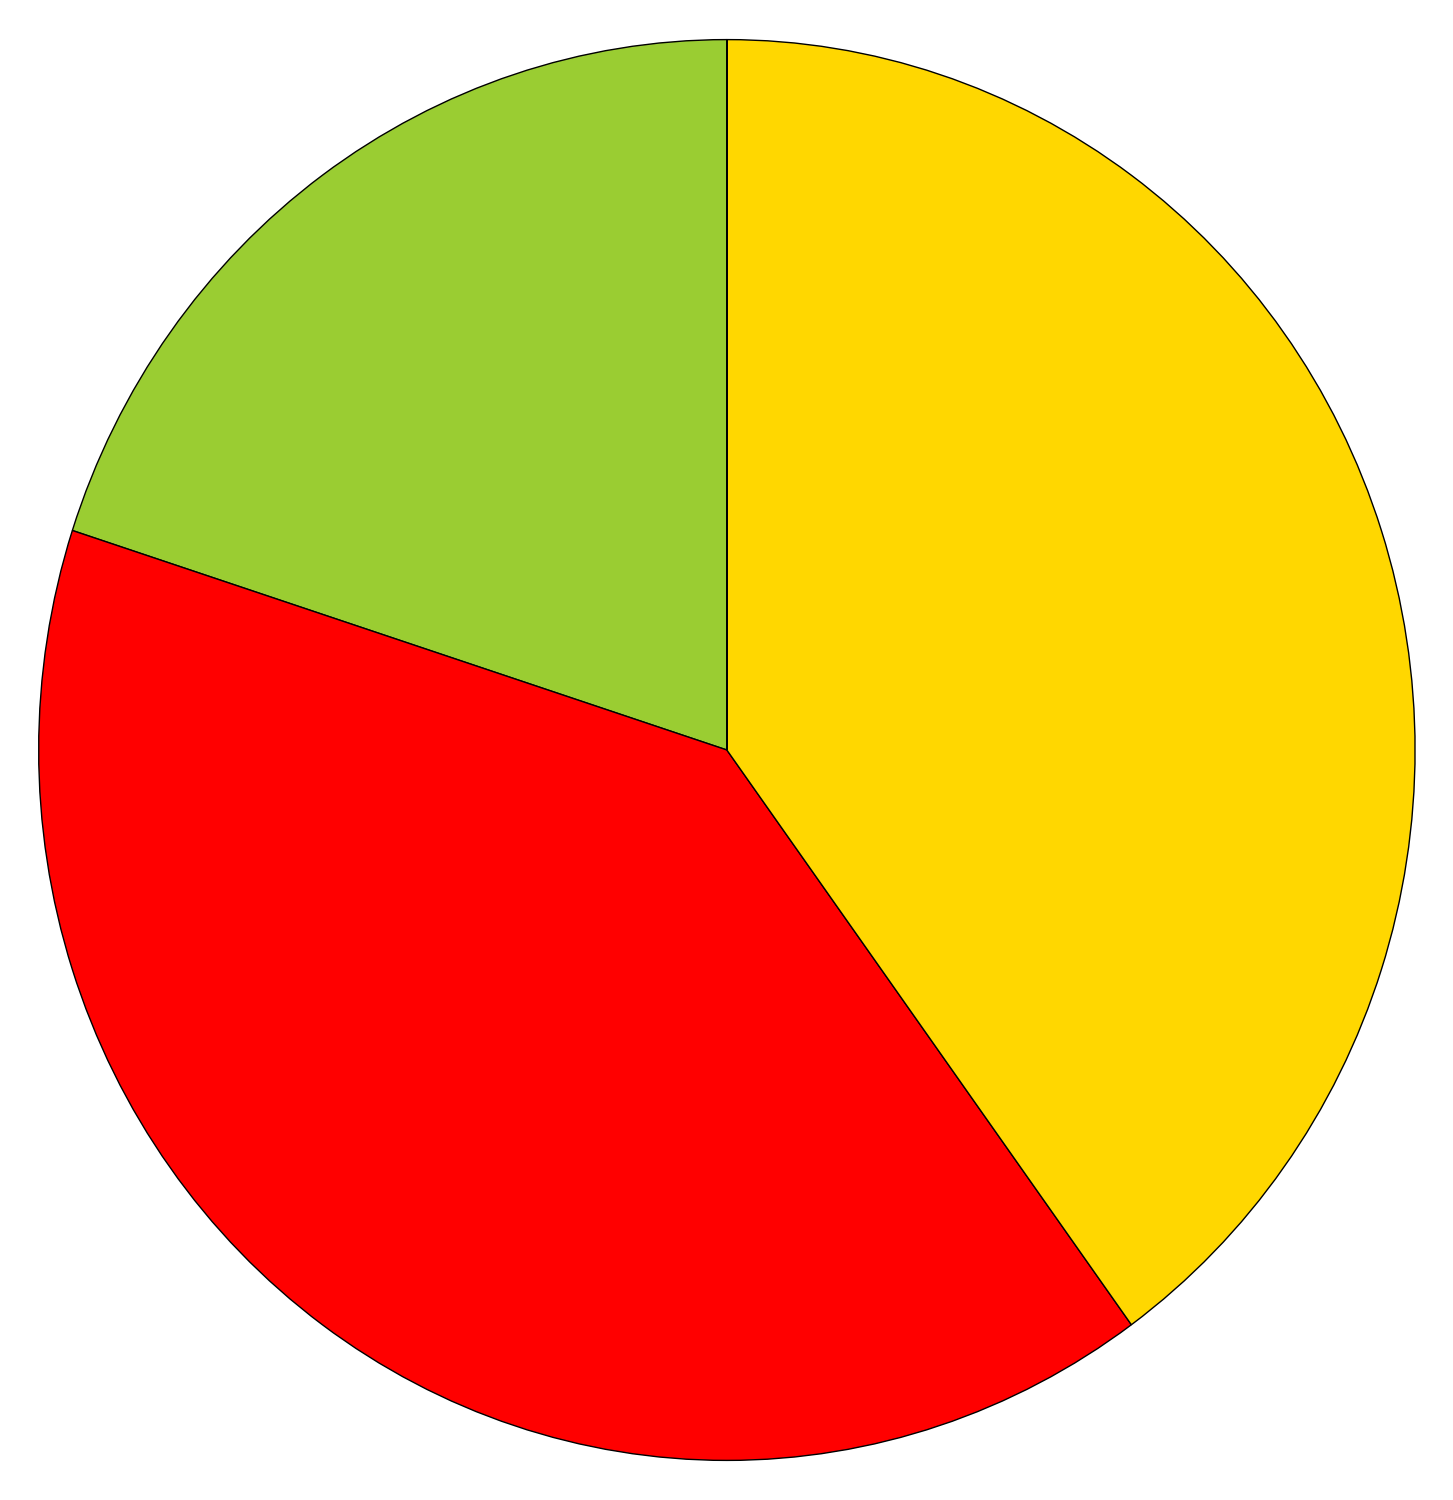
\includegraphics[width=\textwidth]{arousalALLpearsonRgen}
    \caption{Pearson correlation}
  \end{subfigure}
  \hfill
  \begin{subfigure}[b]{0.3\textwidth}
    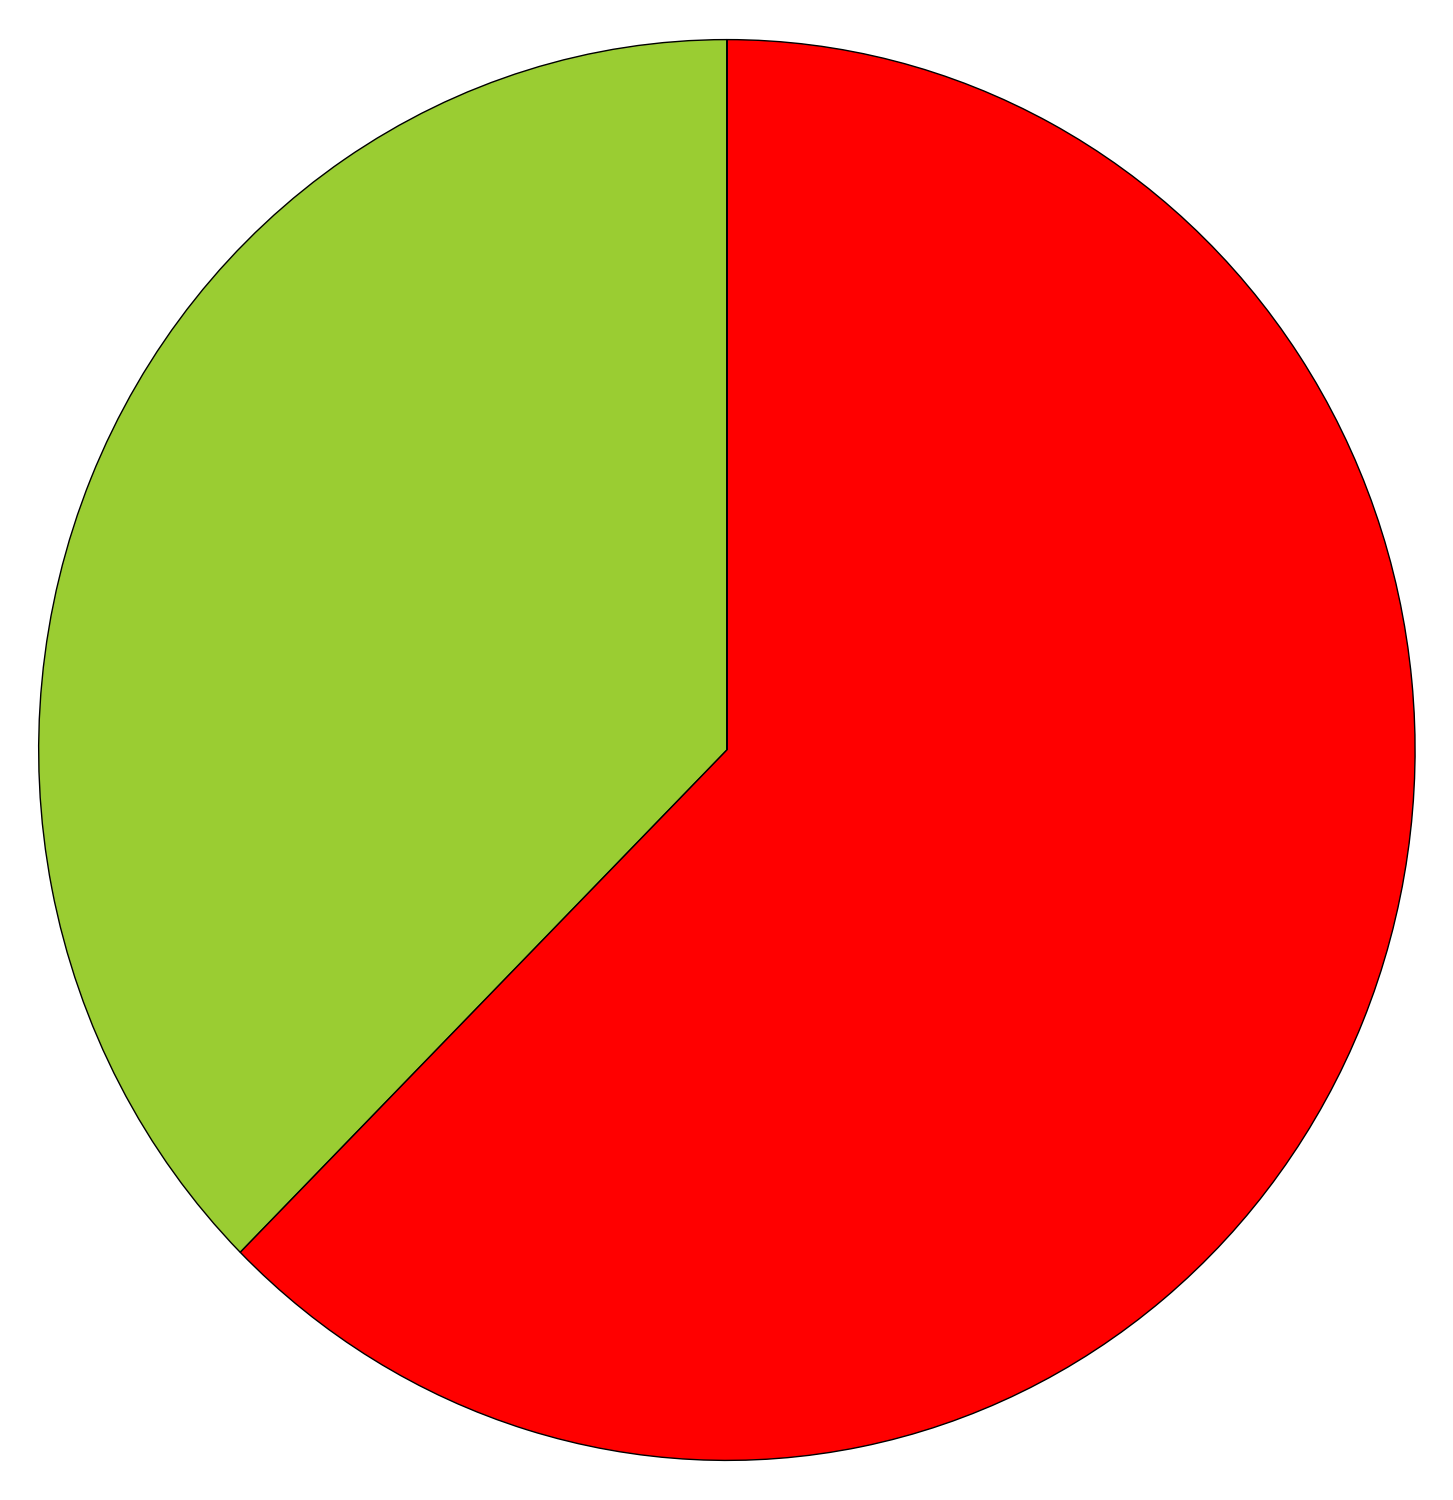
\includegraphics[width=\textwidth]{arousalALLMutInfgen}
    \caption{Mutual information}
  \end{subfigure}
  \hfill
  \begin{subfigure}[b]{0.3\textwidth}
    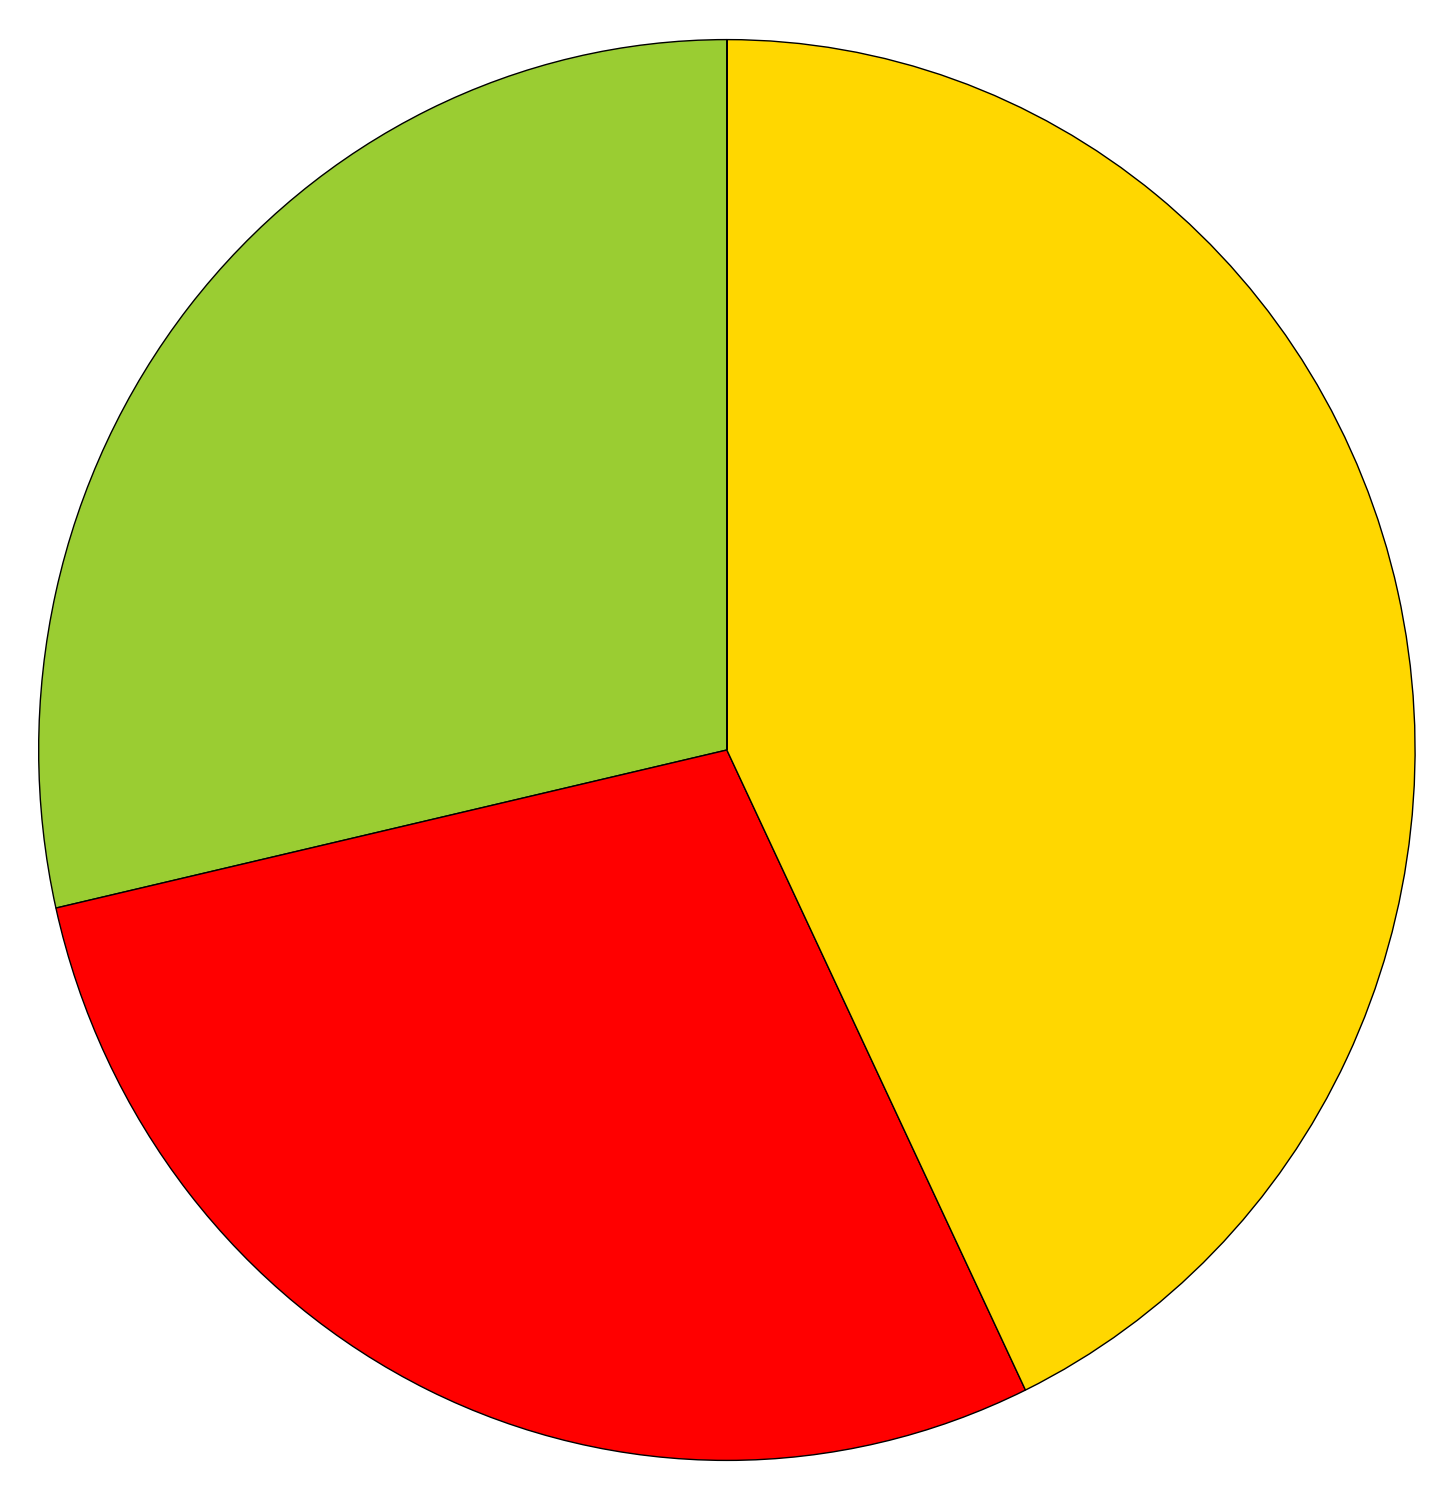
\includegraphics[width=\textwidth]{arousalALLdCorrgen}
    \caption{Distance Correlation}
  \end{subfigure}
  
  \begin{subfigure}[b]{0.3\textwidth}
    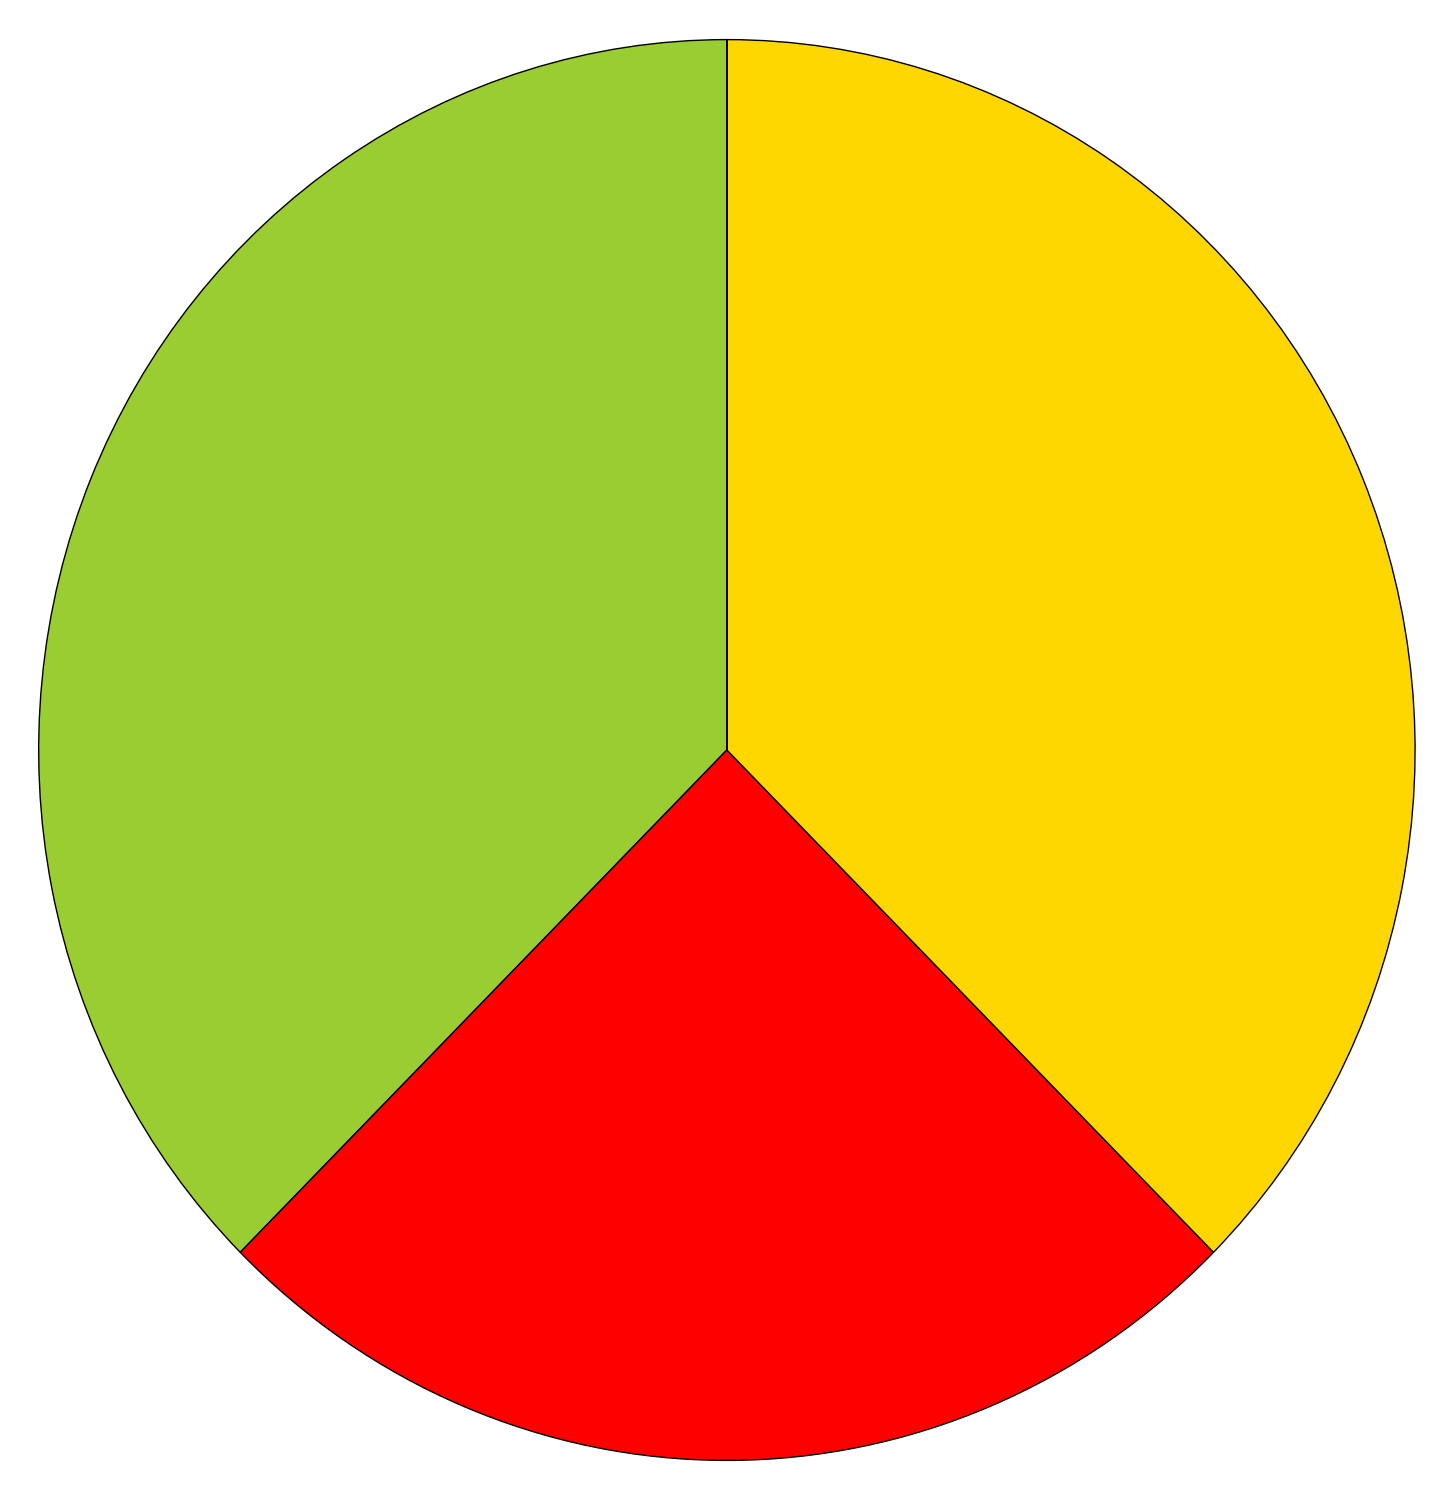
\includegraphics[width=\textwidth]{arousalALLANOVAgen}
    \caption{ANOVA}
  \end{subfigure}
  \hfill
  \begin{subfigure}[b]{0.3\textwidth}
    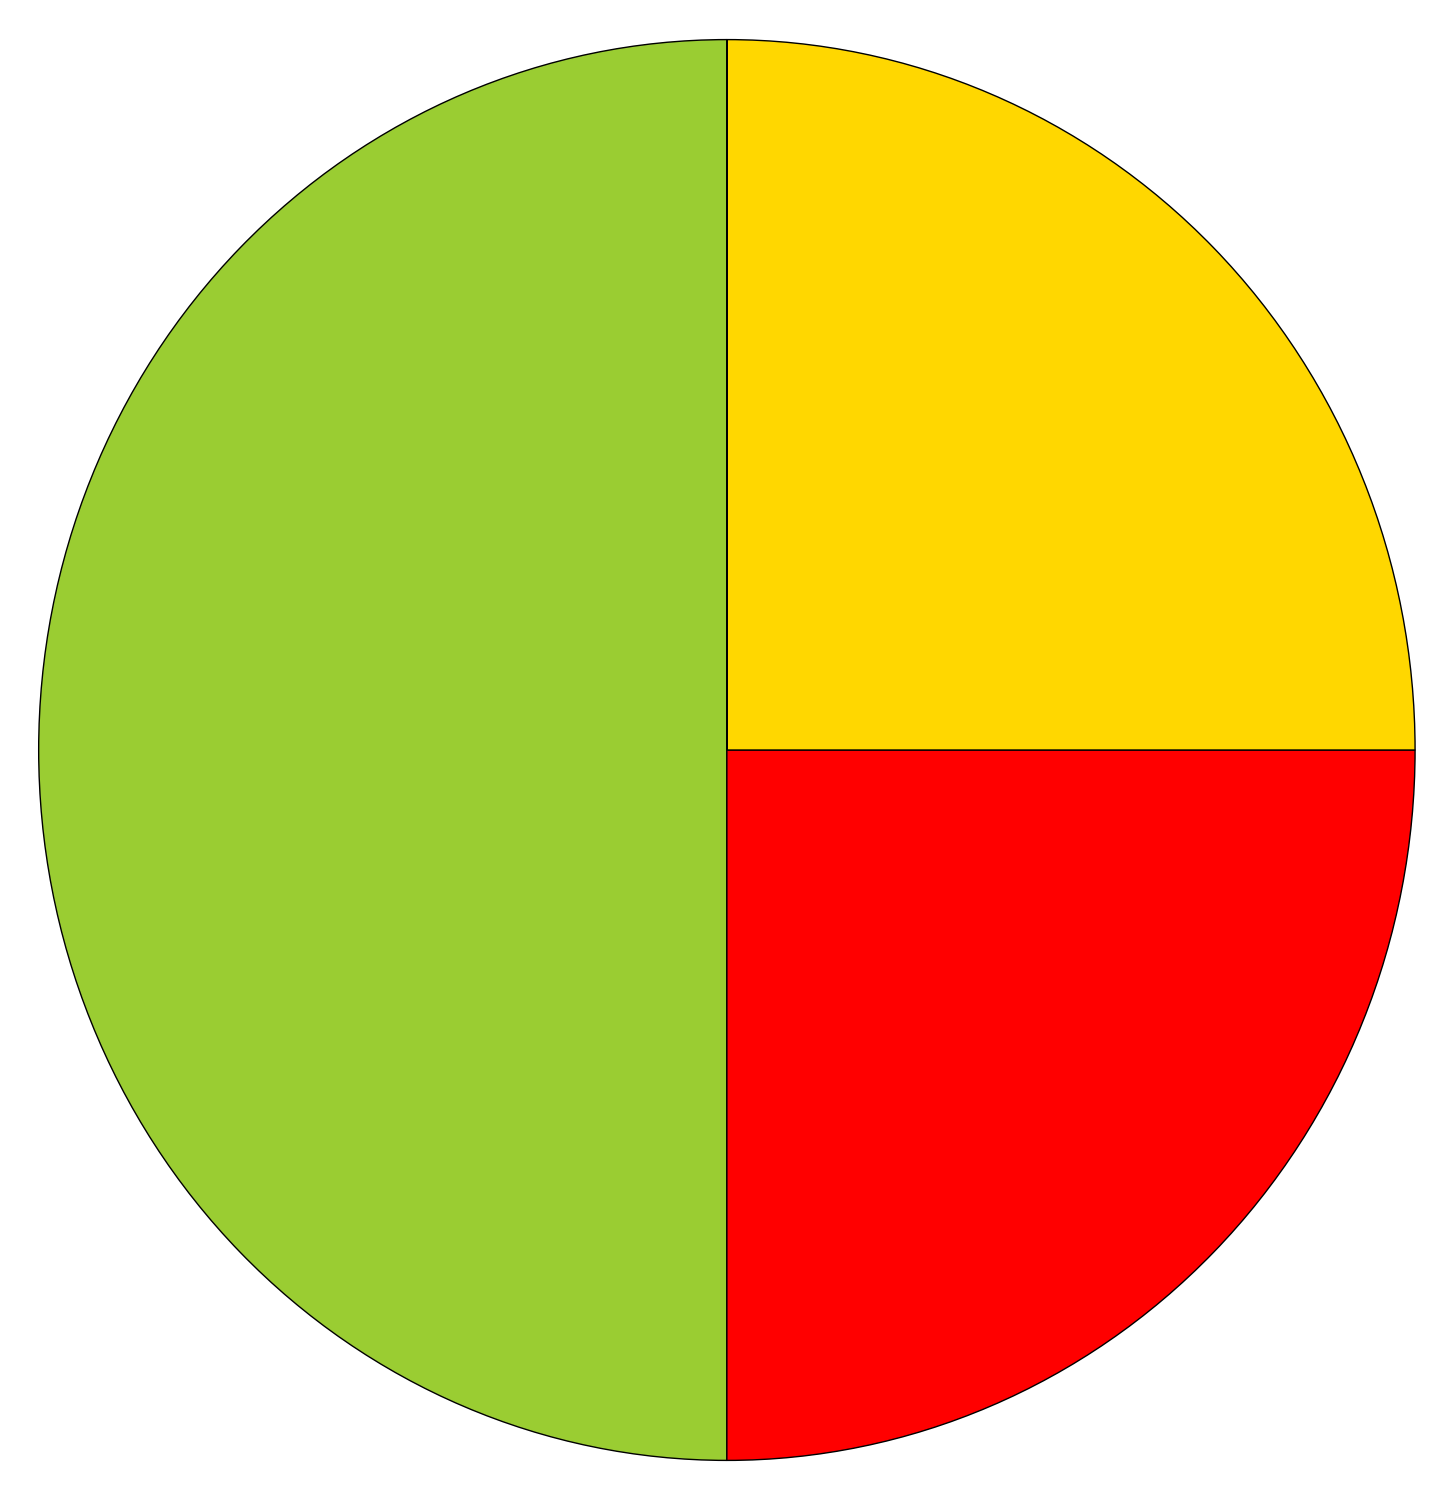
\includegraphics[width=\textwidth]{arousalALLLRgen}
    \caption{Linear regression}
  \end{subfigure}
  \hfill
  \begin{subfigure}[b]{0.3\textwidth}
    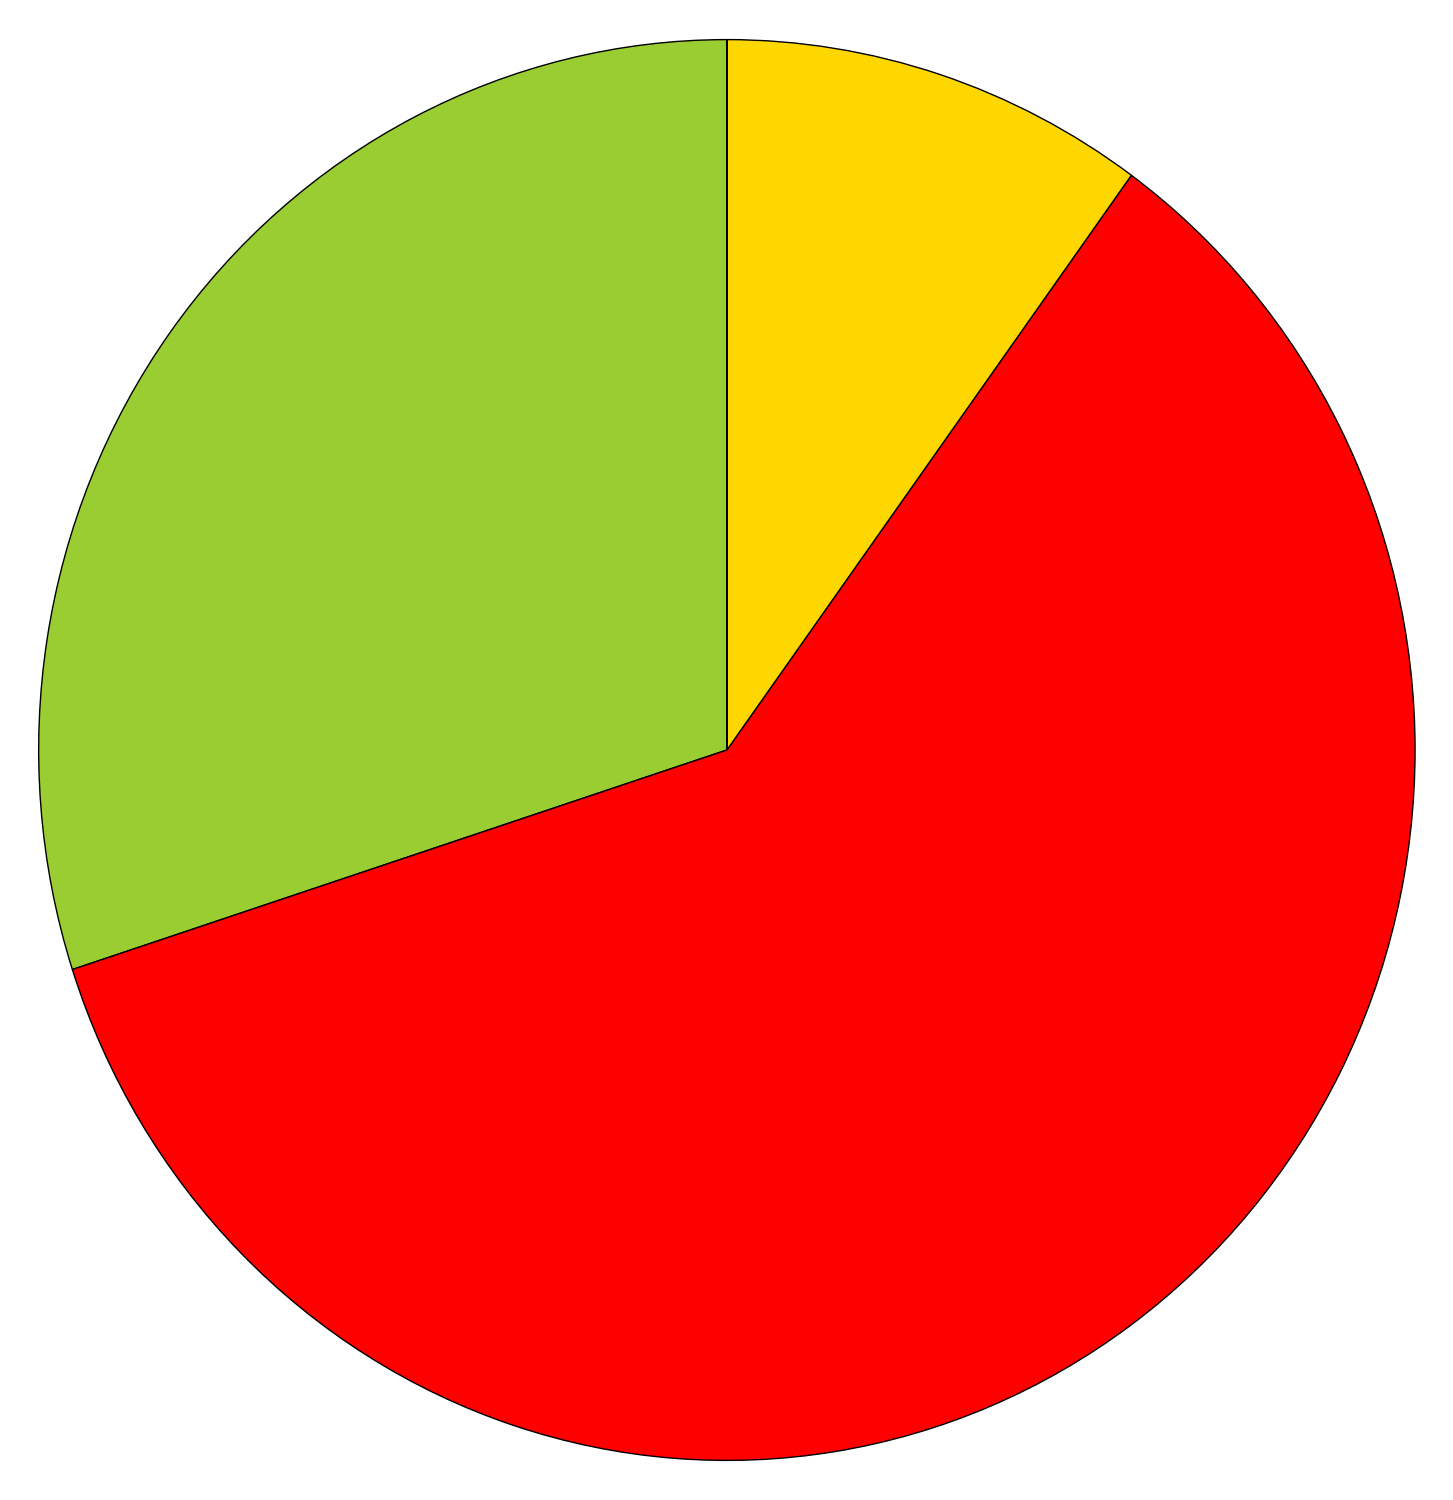
\includegraphics[width=\textwidth]{arousalALLSVMgen}
    \caption{SVM}
  \end{subfigure}
  
  \begin{subfigure}[b]{0.3\textwidth}
    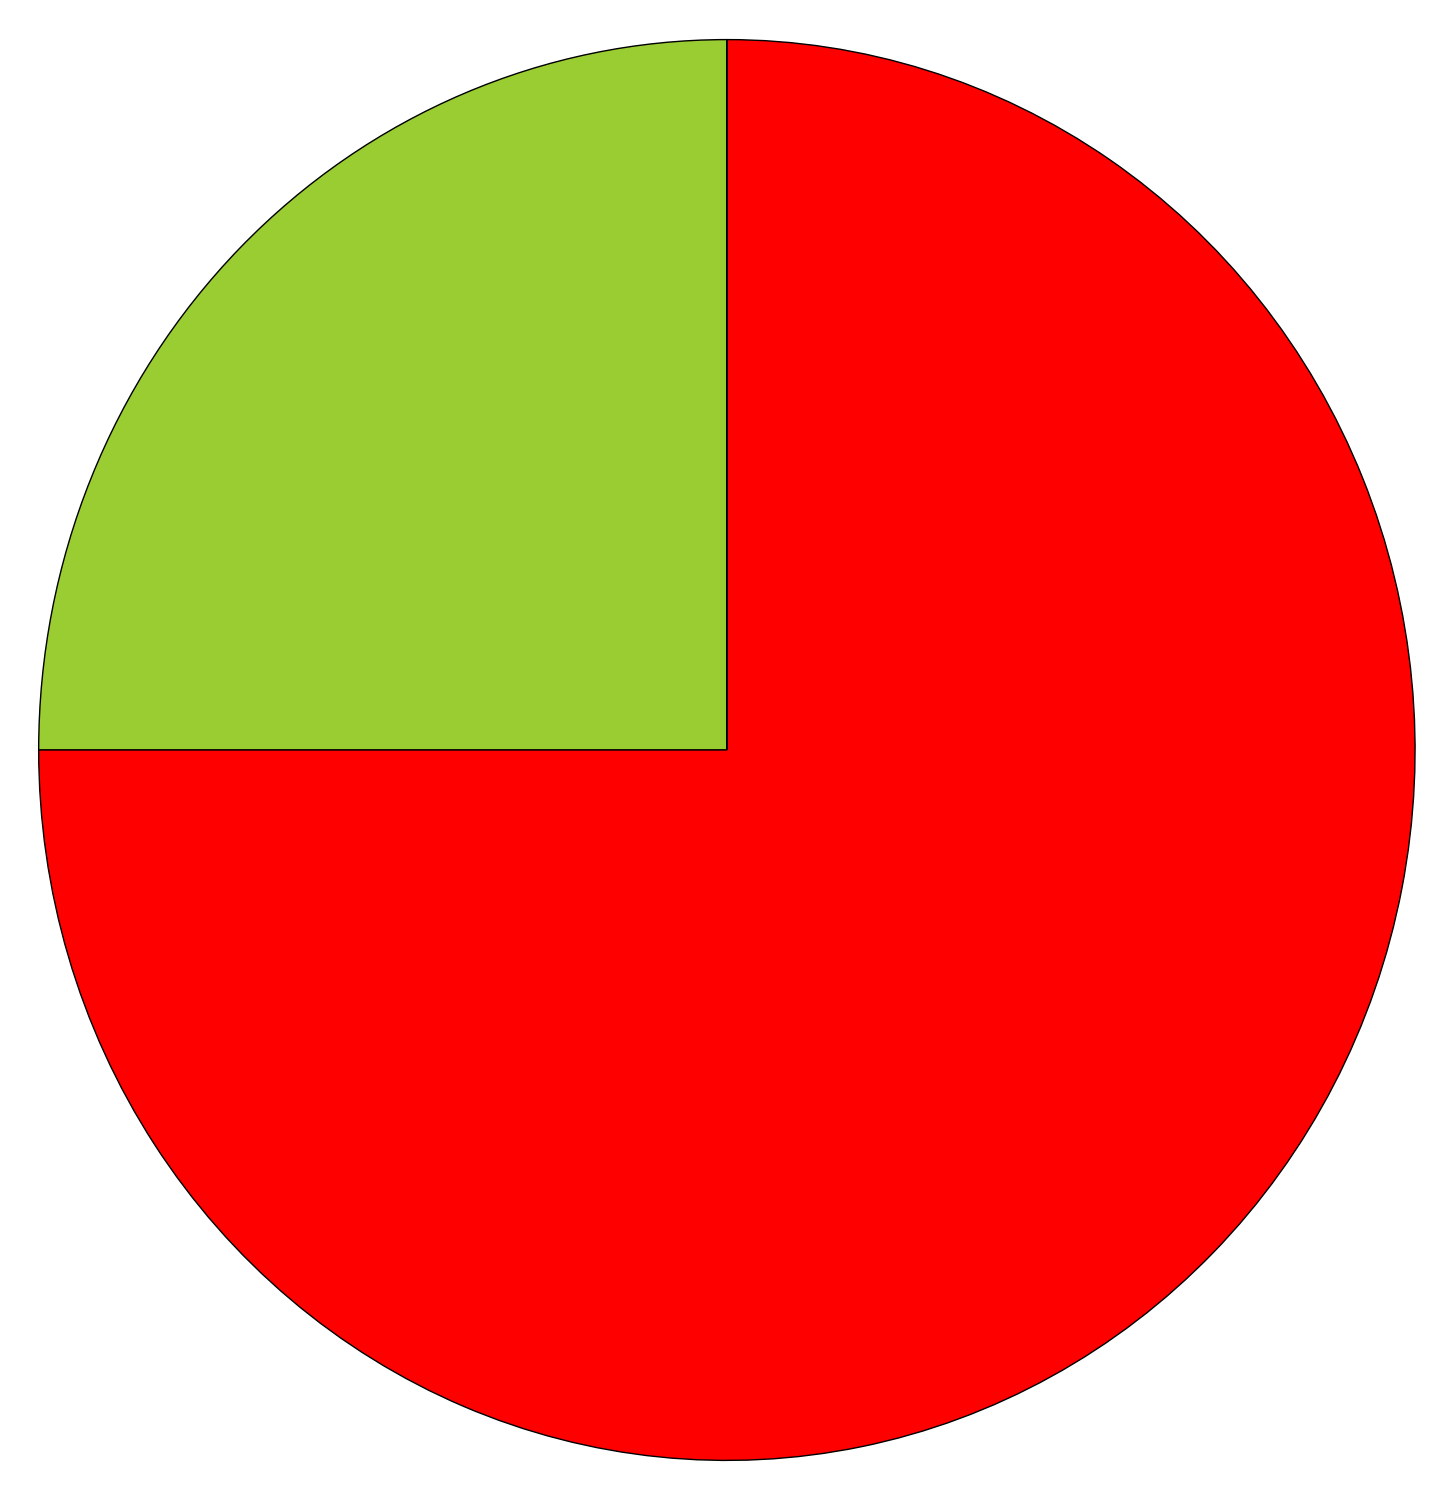
\includegraphics[width=\textwidth]{arousalALLLDAgen}
    \caption{LDA}
  \end{subfigure}
  \hfill
  \begin{subfigure}[b]{0.3\textwidth}
    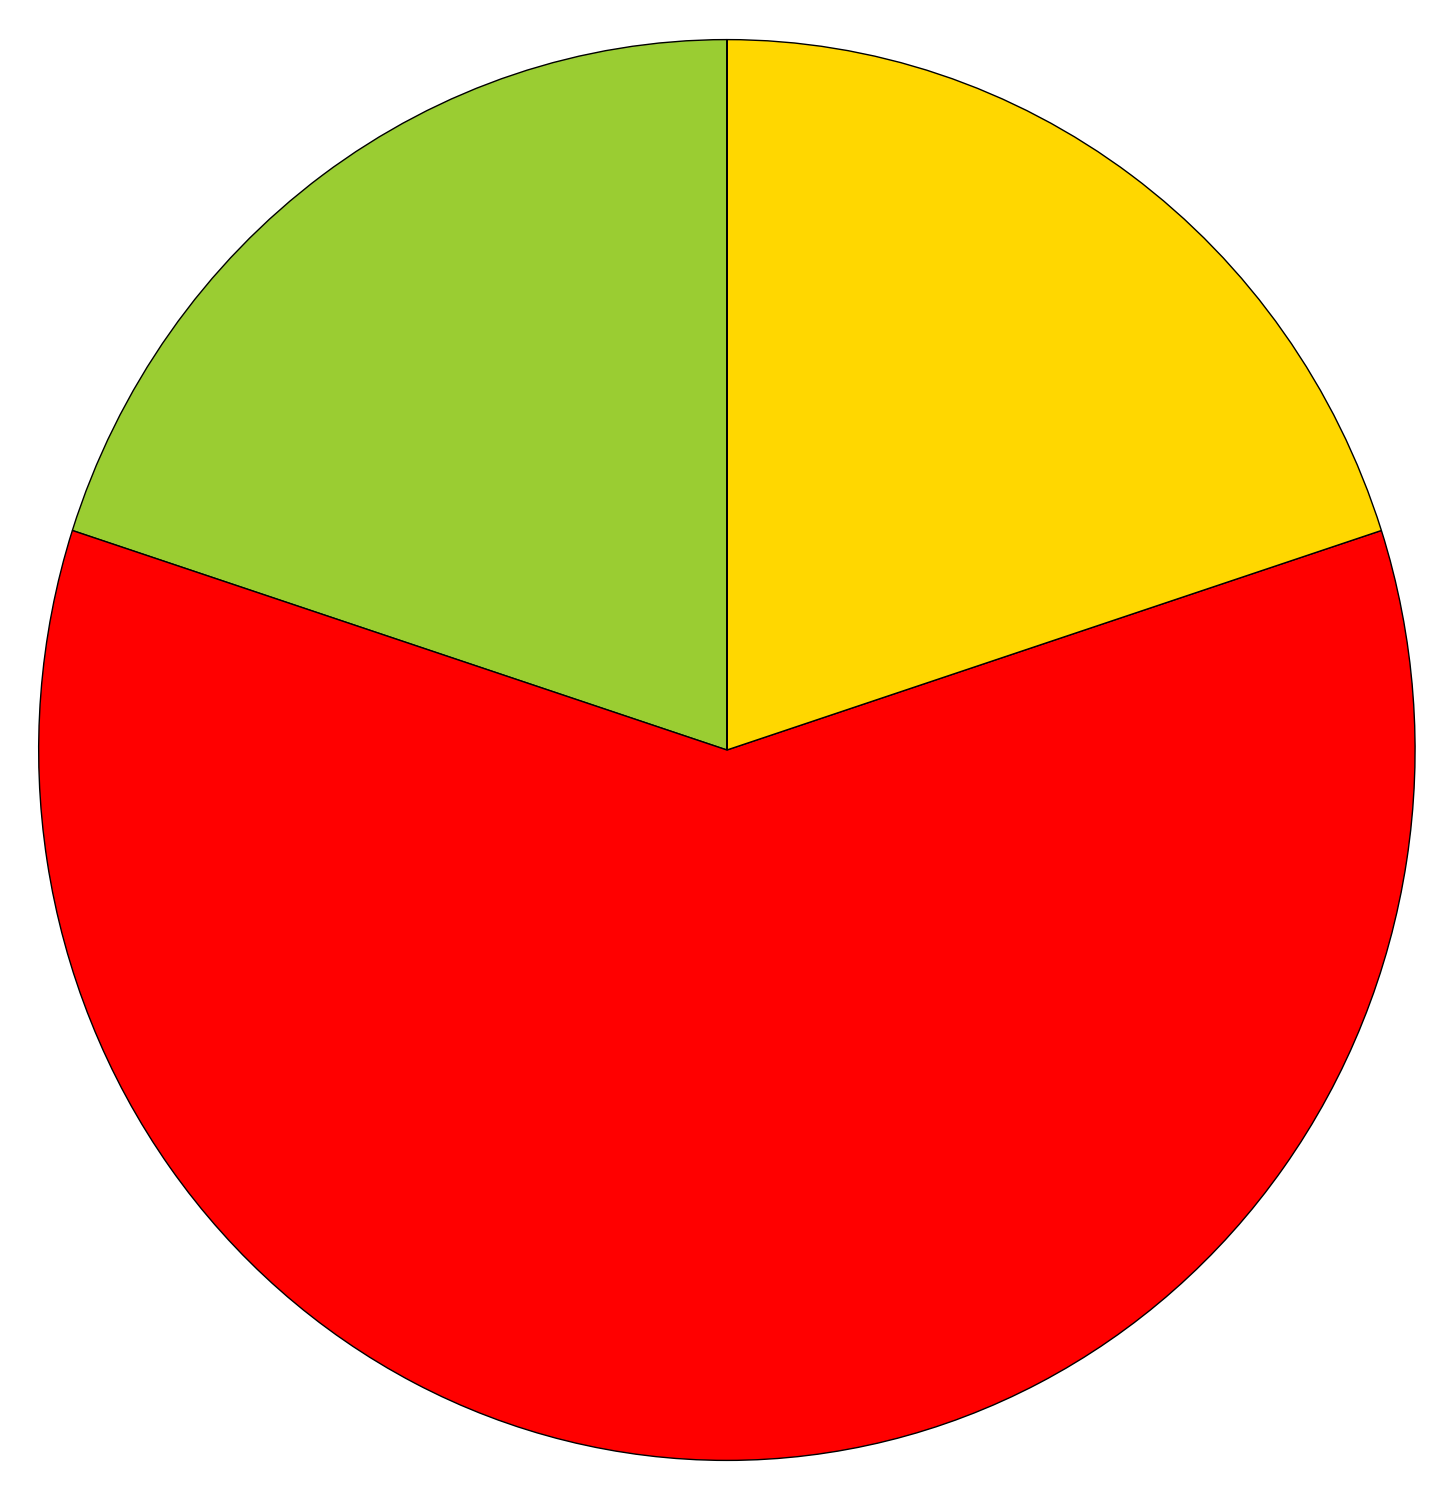
\includegraphics[width=\textwidth]{arousalALLL1gen}
    \caption{Lasso regression}
  \end{subfigure}
  \hfill
  \begin{subfigure}[b]{0.3\textwidth}
    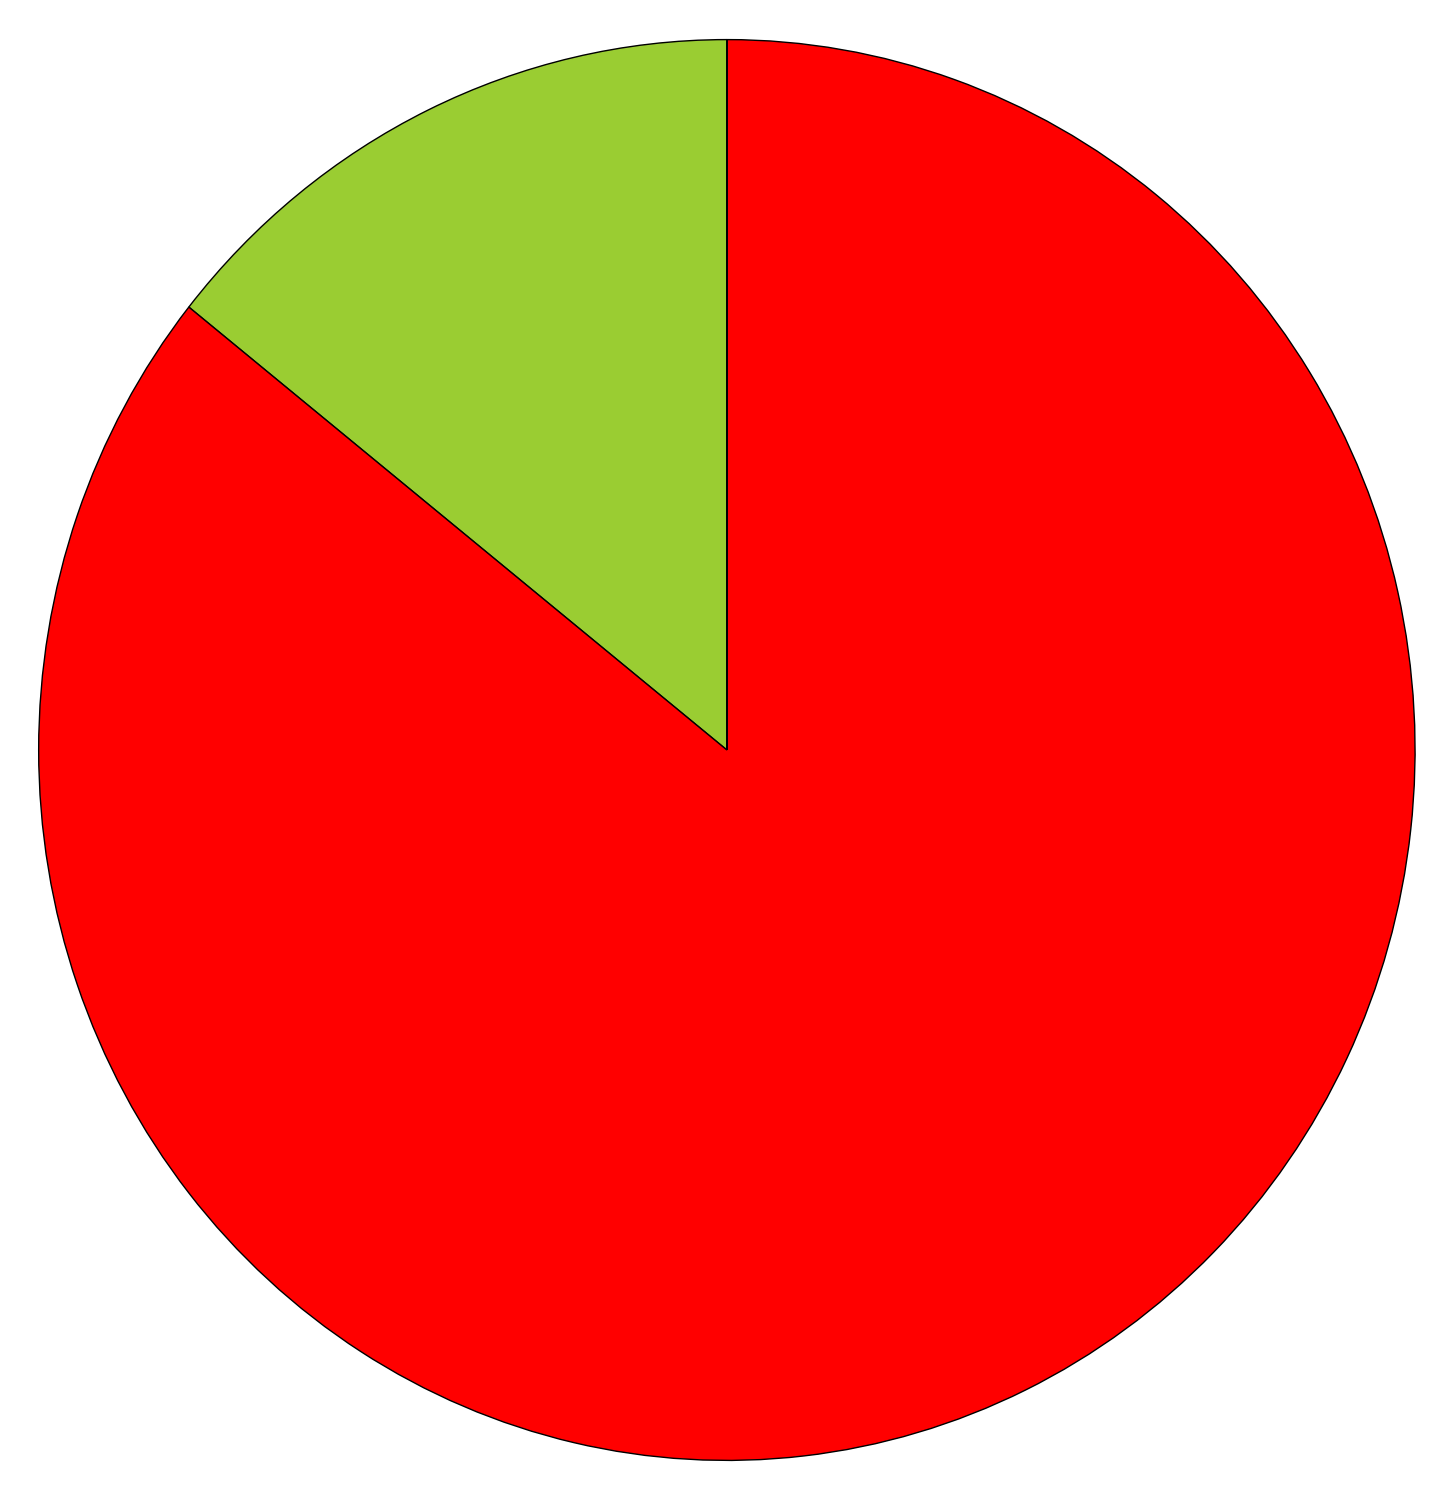
\includegraphics[width=\textwidth]{arousalALLL2gen}
    \caption{Ridge regression}
  \end{subfigure}
  
  \begin{subfigure}[b]{0.3\textwidth}
    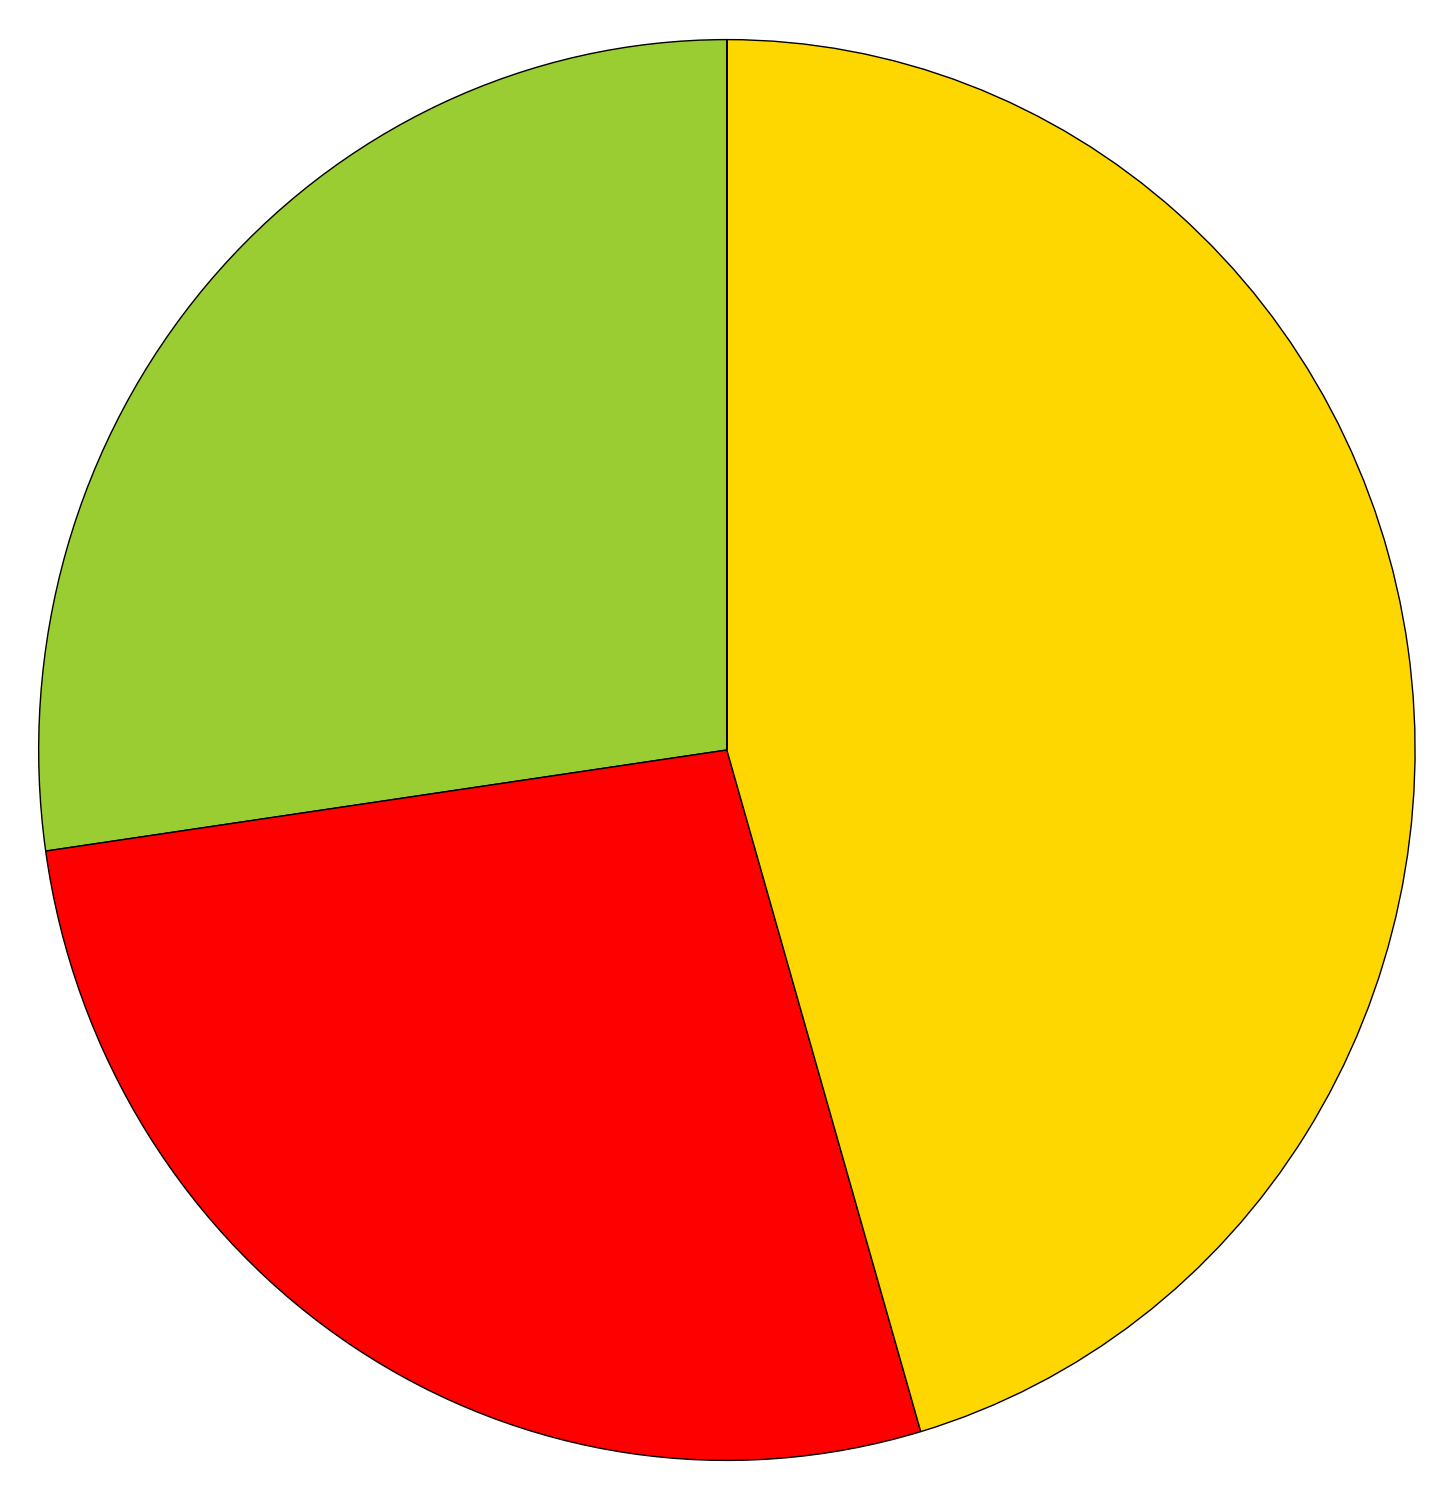
\includegraphics[width=\textwidth]{arousalALLRFgen}
    \caption{Random forests}
  \end{subfigure}
  \hfill
  \begin{subfigure}[b]{0.3\textwidth}
    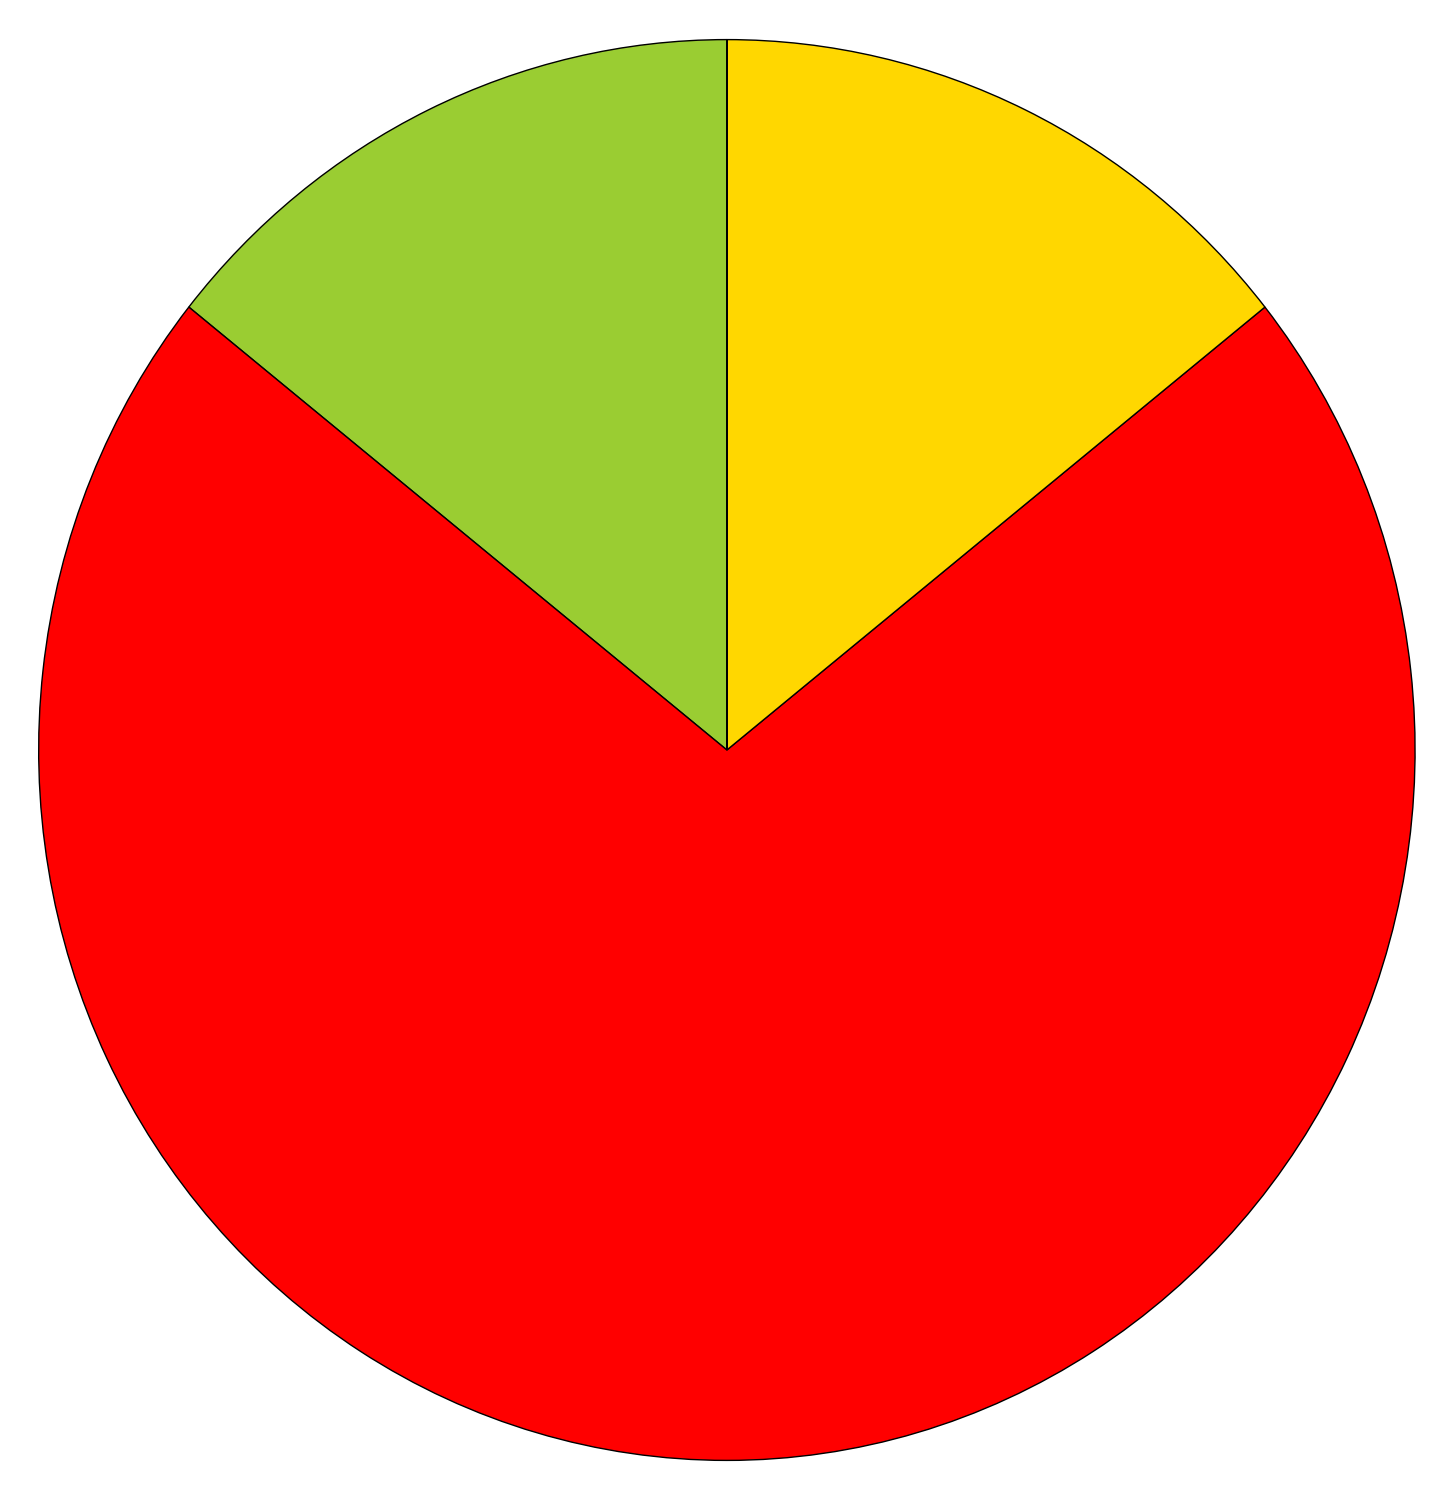
\includegraphics[width=\textwidth]{arousalALLPCAgen}
    \caption{PCA}
  \end{subfigure}
  \hfill
  \begin{subfigure}[b]{0.3\textwidth}
    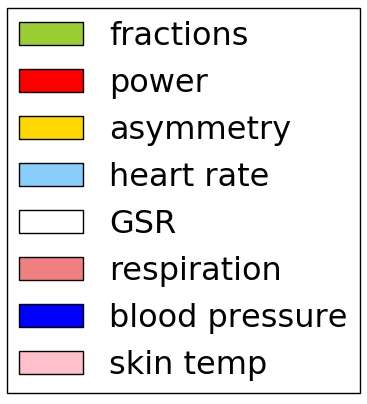
\includegraphics[width=\textwidth]{legend}
    \caption{Legend\label{arousalpieslegendgen}}
  \end{subfigure}
\end{figure}

\clearpage

\begin{figure}[!tbp]
  \centering
  \caption{Selection features for valence classification.\label{valencepiesgen}}
  \begin{subfigure}[b]{0.3\textwidth}
    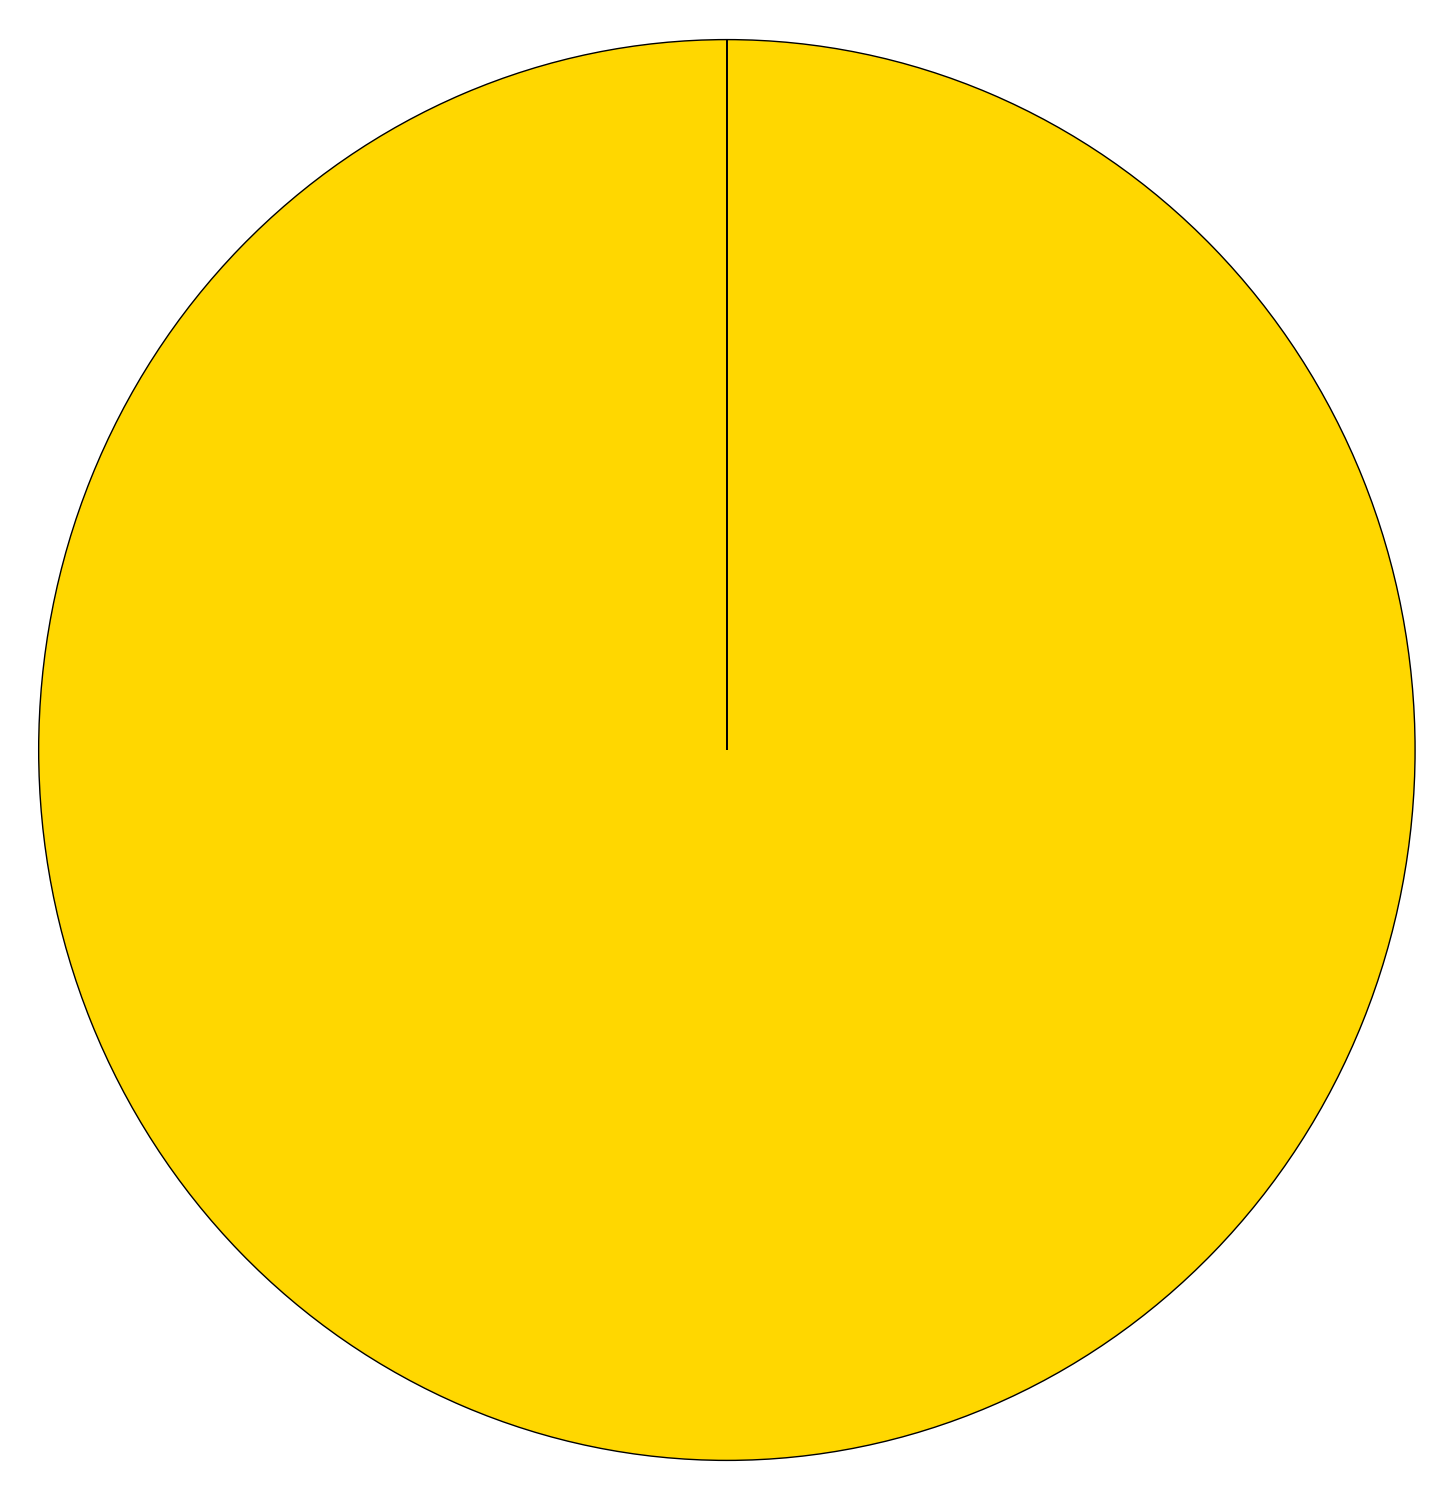
\includegraphics[width=\textwidth]{valenceALLpearsonRgen}
    \caption{Pearson correlation}
  \end{subfigure}
  \hfill
  \begin{subfigure}[b]{0.3\textwidth}
    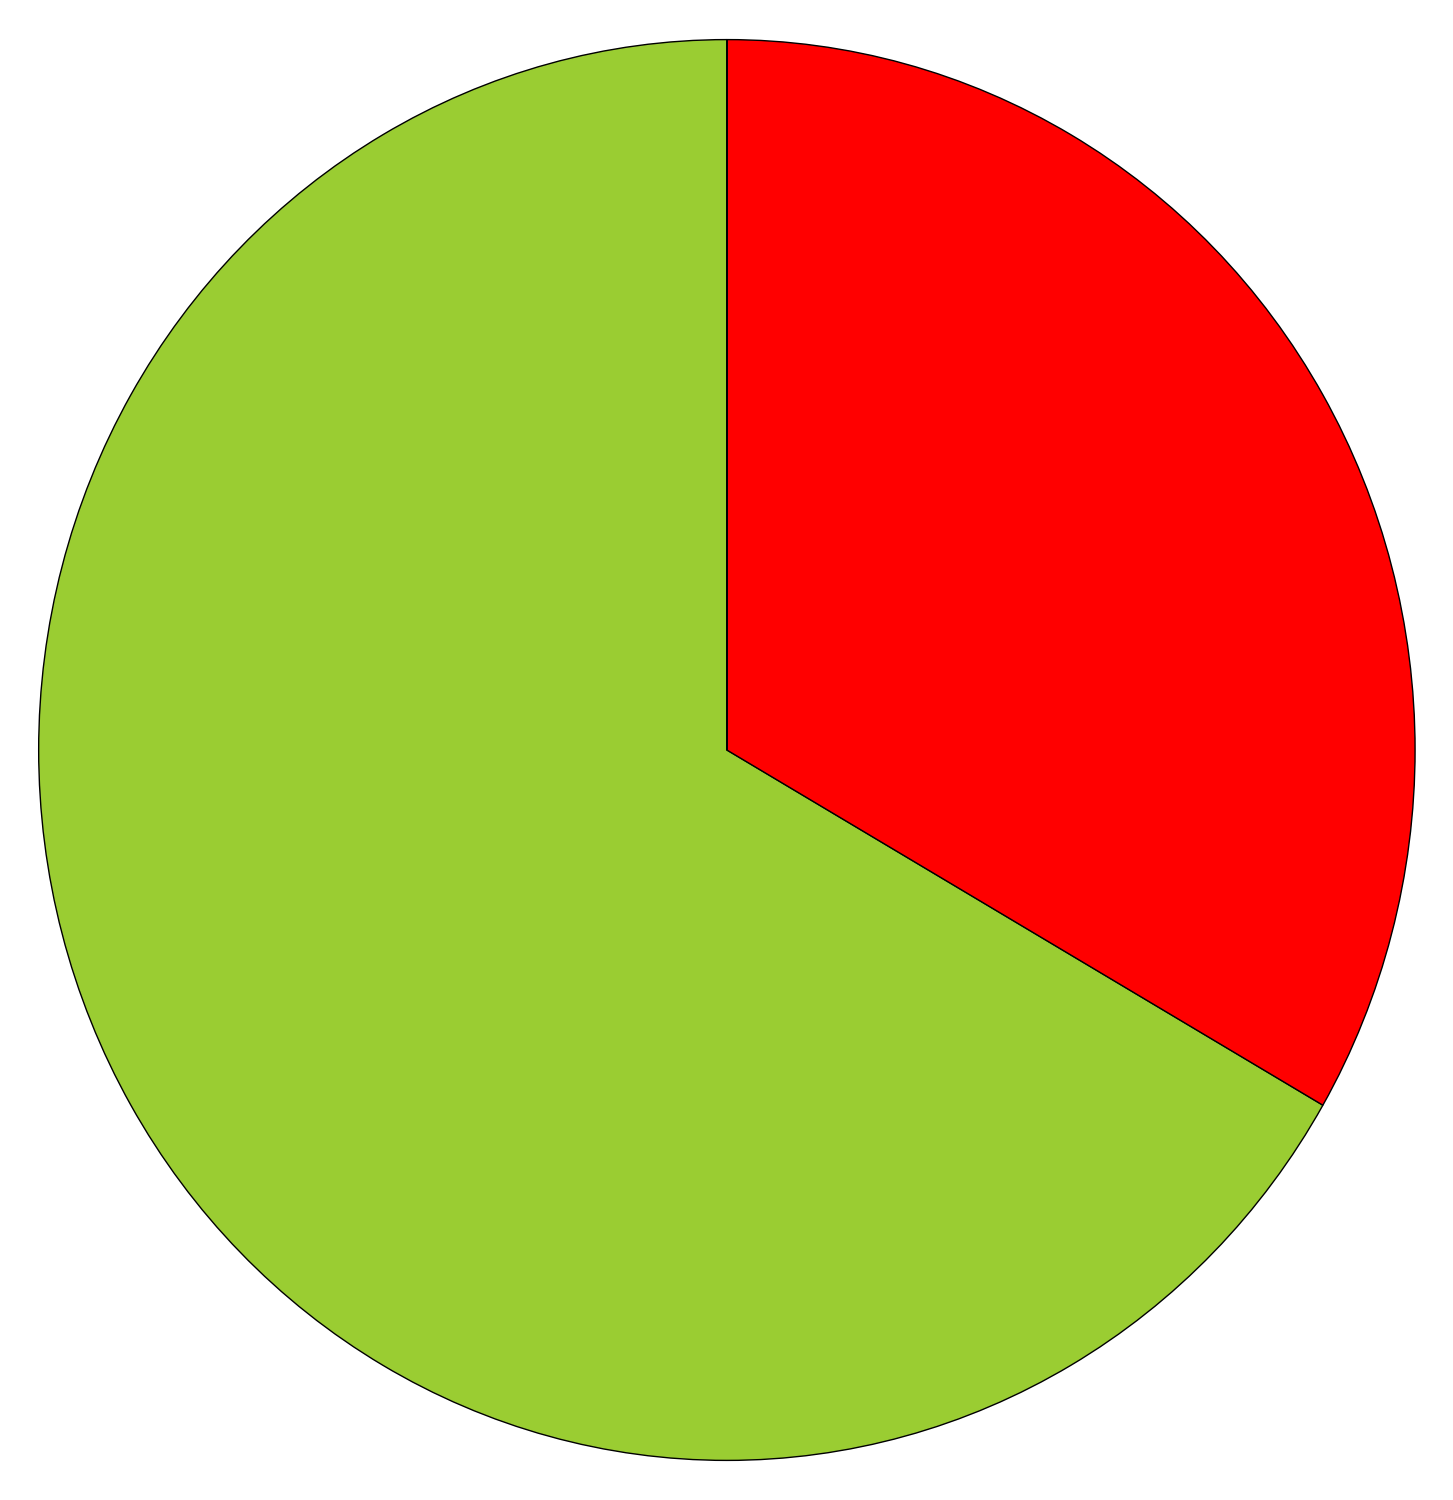
\includegraphics[width=\textwidth]{valenceALLMutInfgen}
    \caption{Mutual information}
  \end{subfigure}
  \hfill
  \begin{subfigure}[b]{0.3\textwidth}
    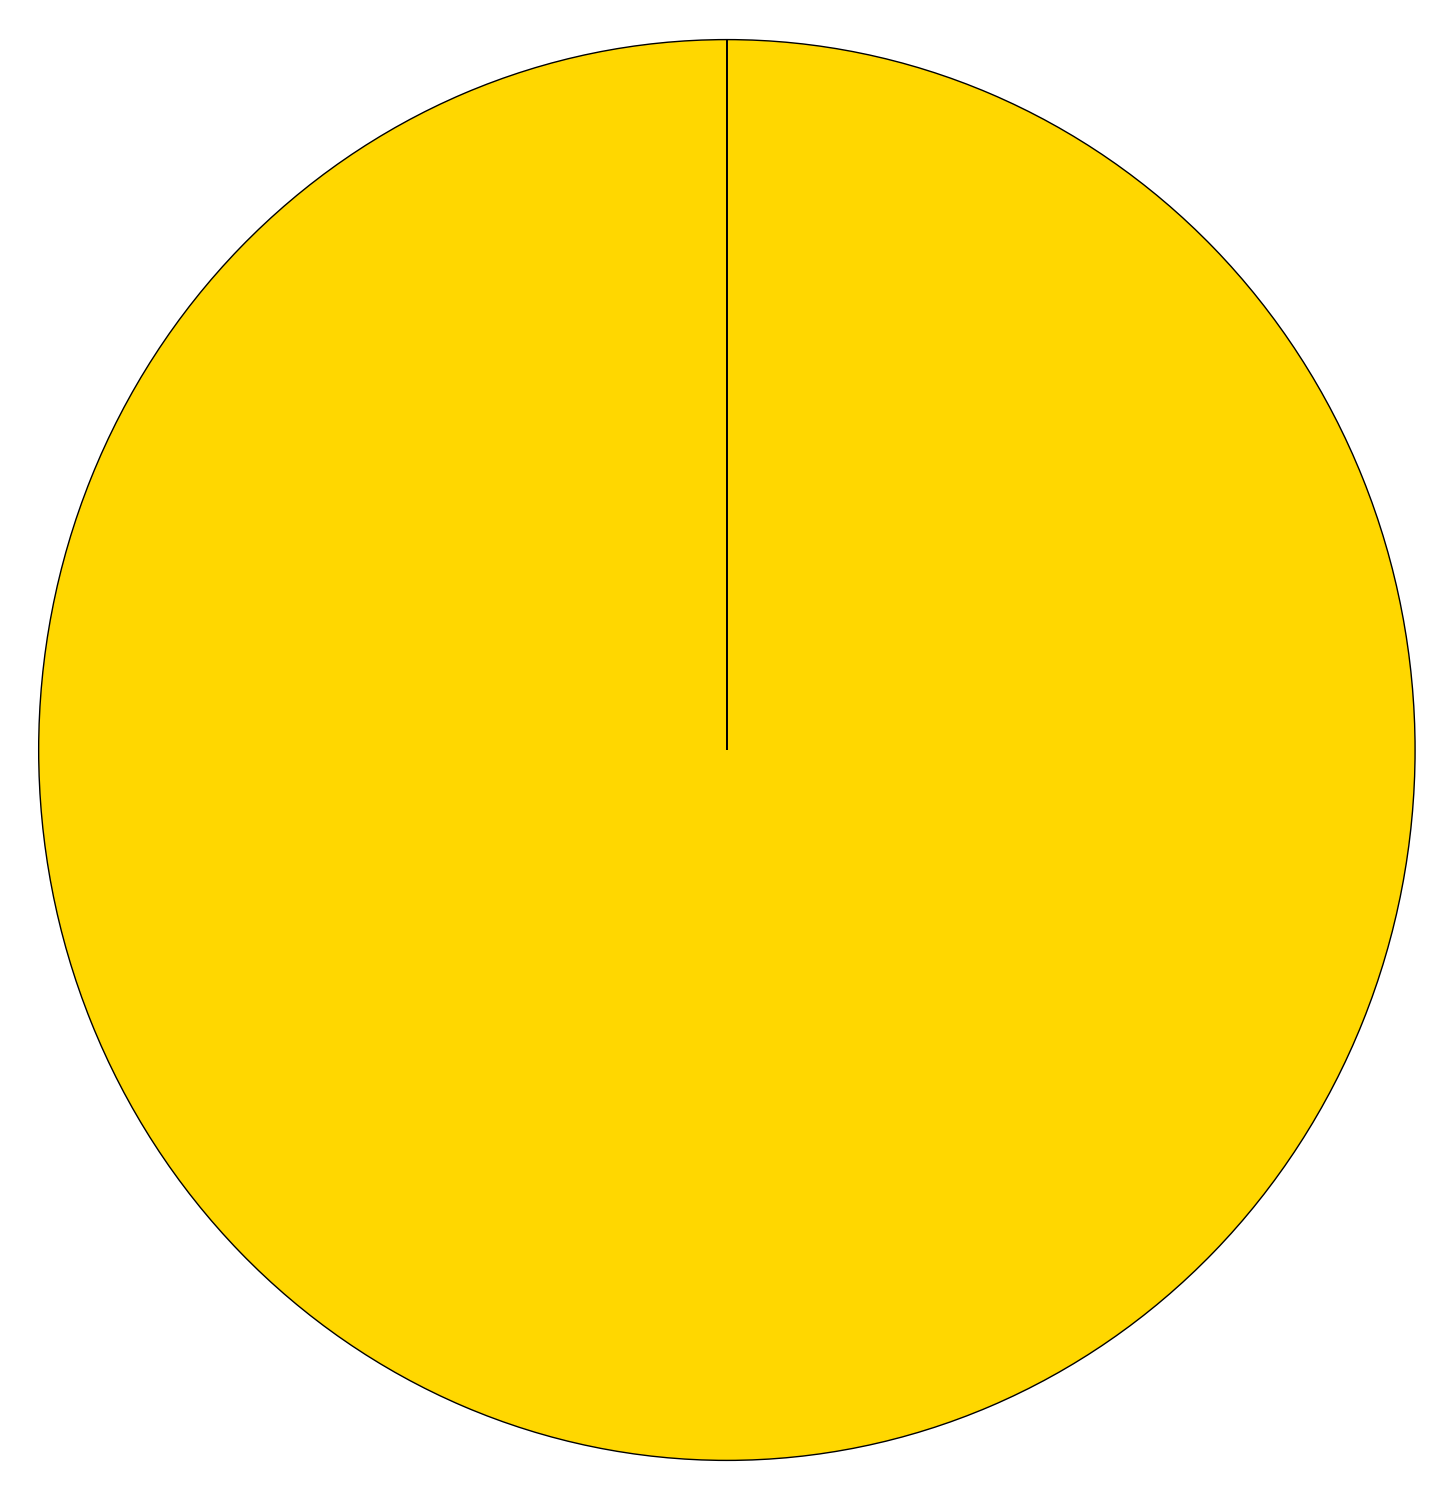
\includegraphics[width=\textwidth]{valenceALLdCorrgen}
    \caption{Distance Correlation}
  \end{subfigure}
  
  \begin{subfigure}[b]{0.3\textwidth}
    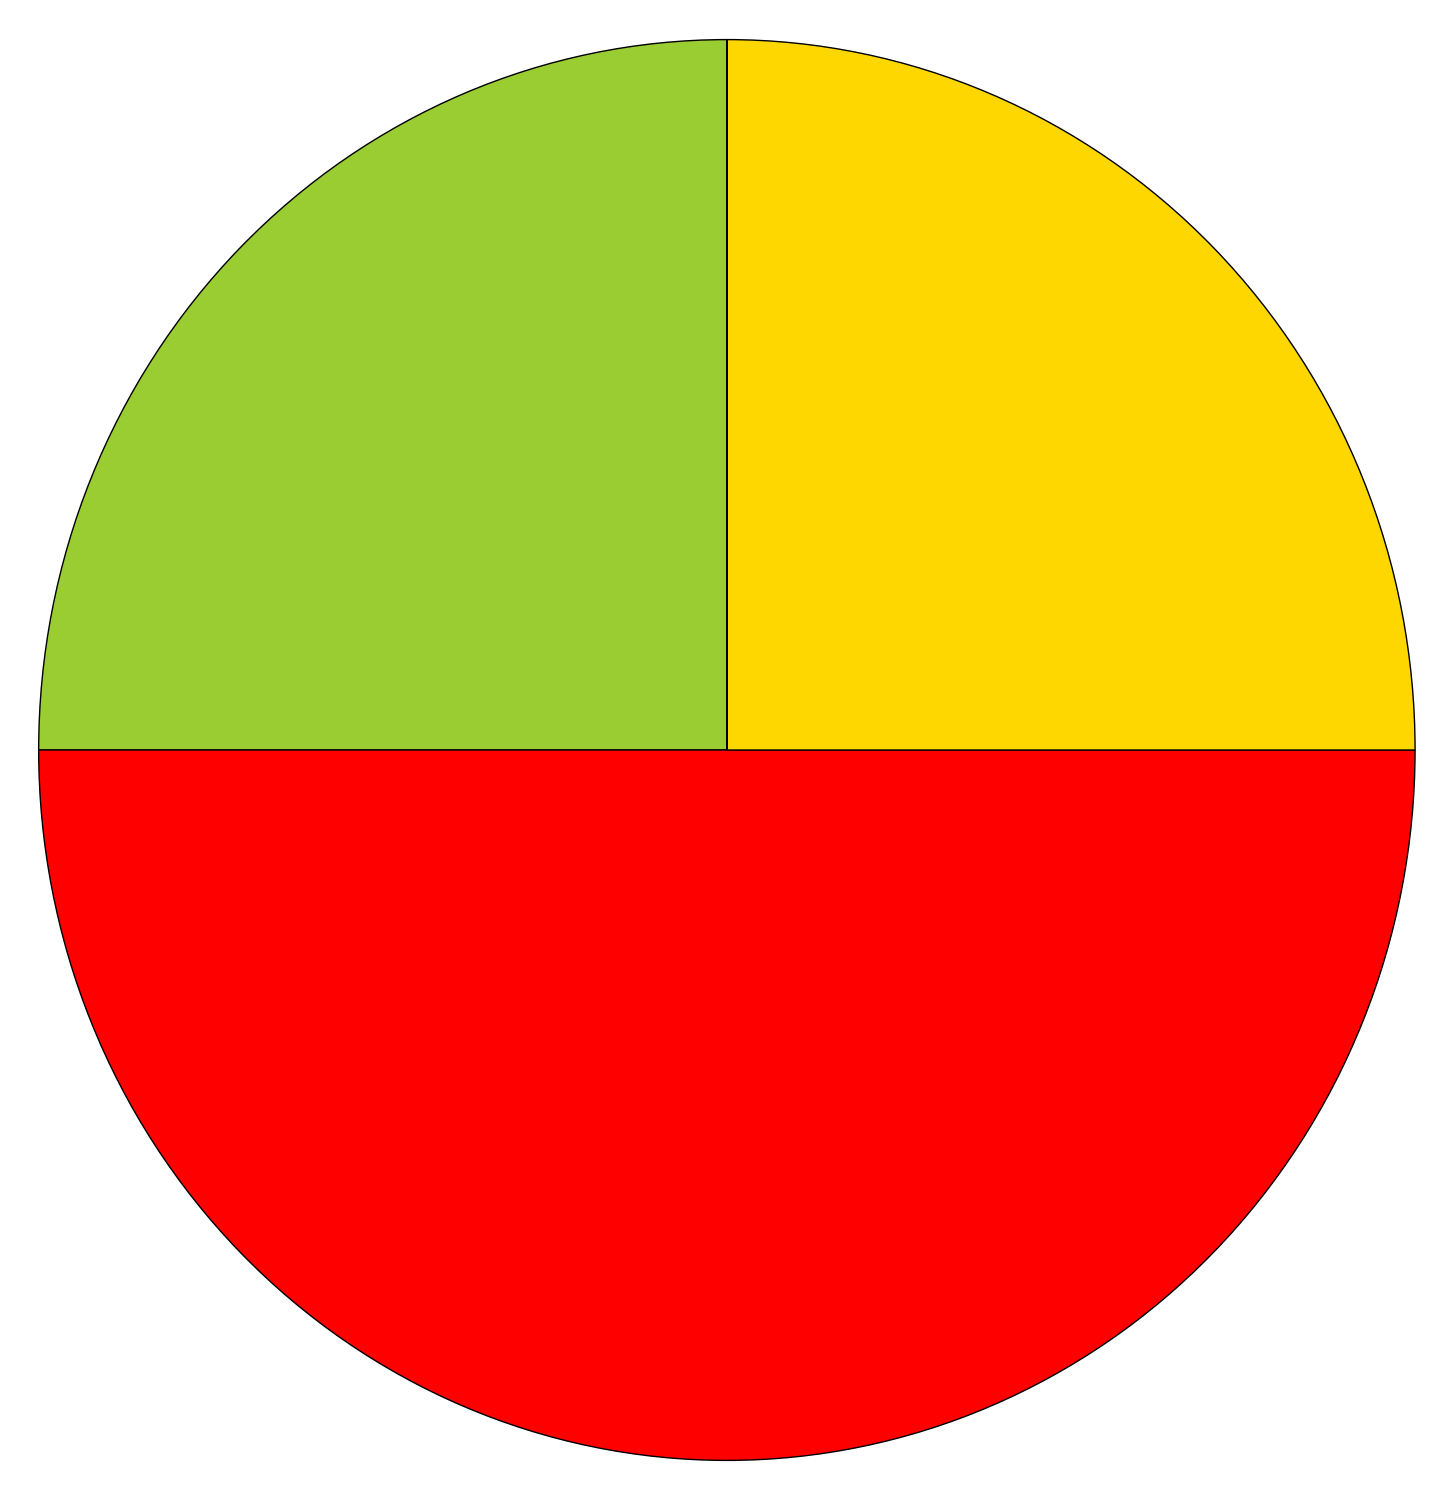
\includegraphics[width=\textwidth]{valenceALLANOVAgen}
    \caption{ANOVA}
  \end{subfigure}
  \hfill
  \begin{subfigure}[b]{0.3\textwidth}
    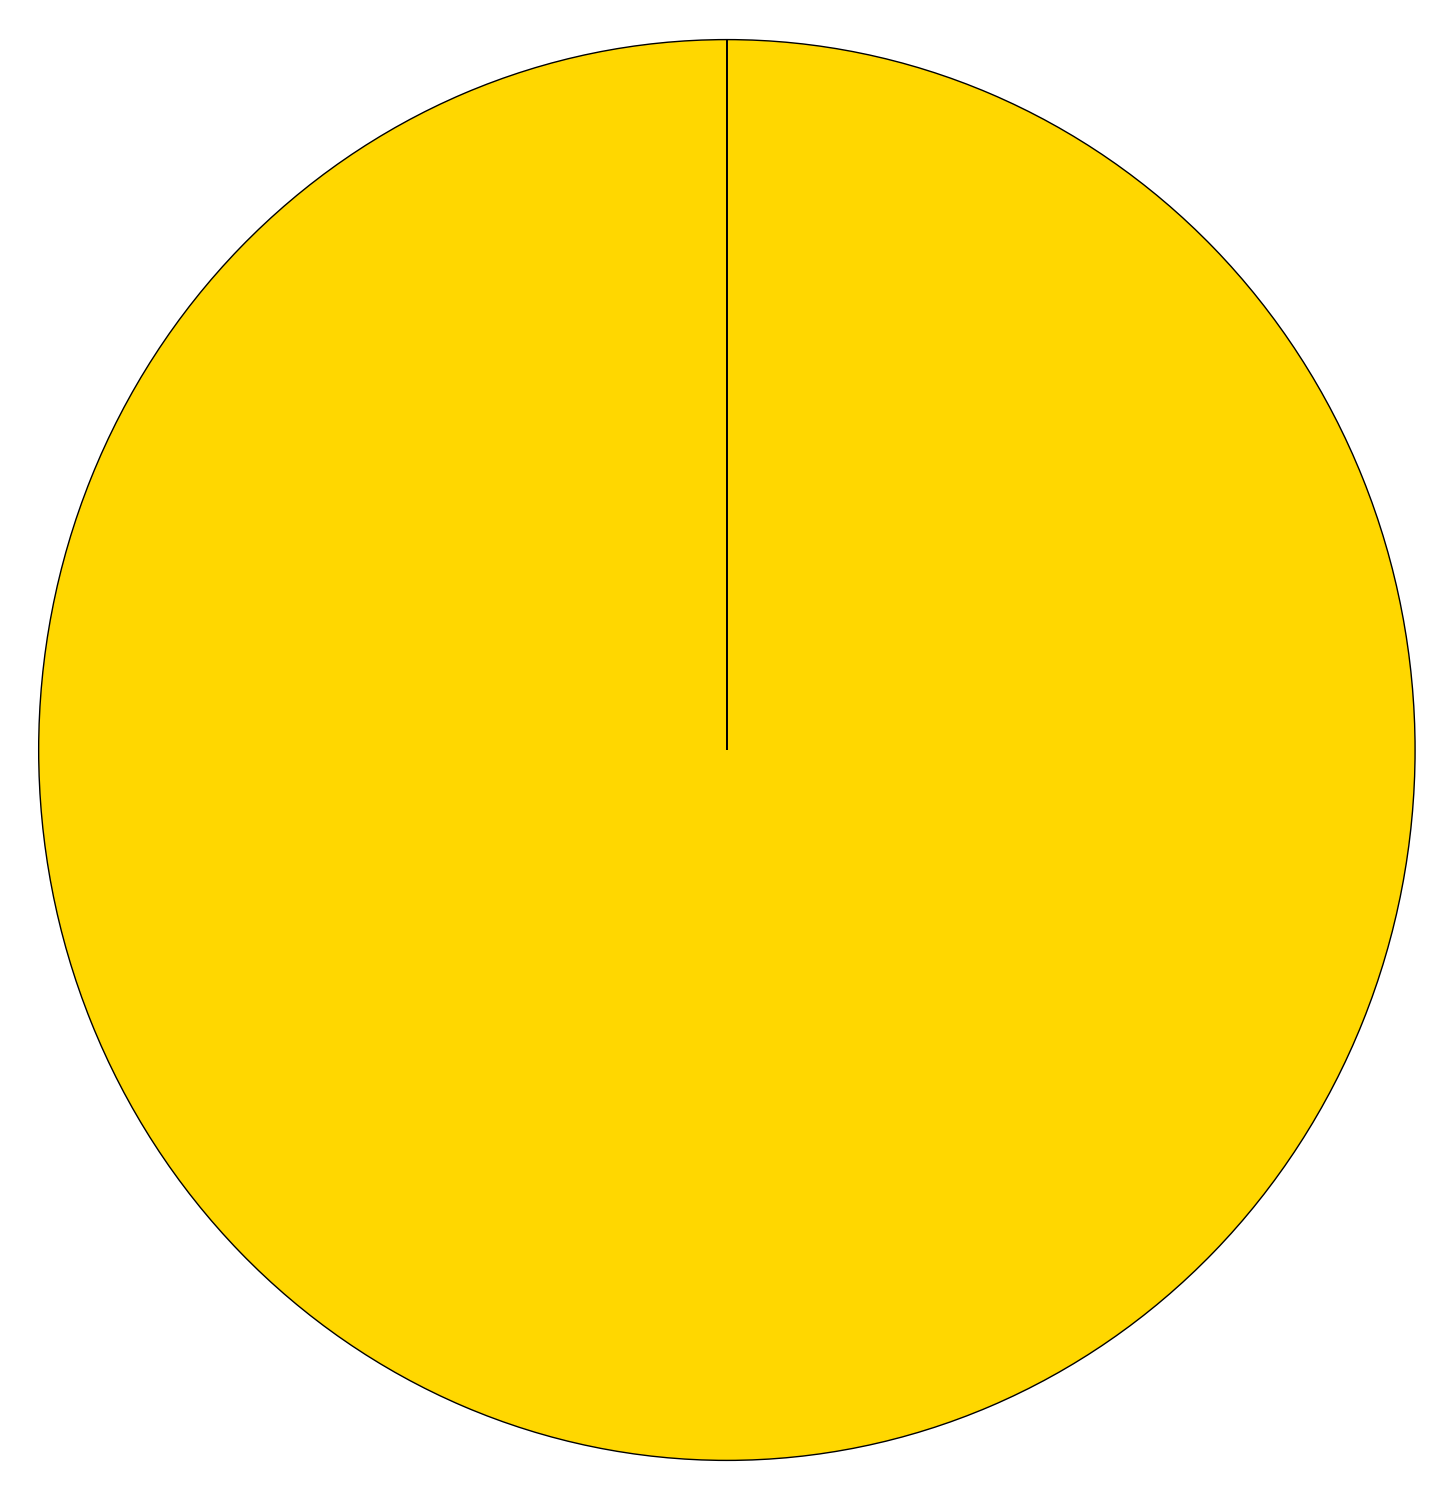
\includegraphics[width=\textwidth]{valenceALLLRgen}
    \caption{Linear regression}
  \end{subfigure}
  \hfill
  \begin{subfigure}[b]{0.3\textwidth}
    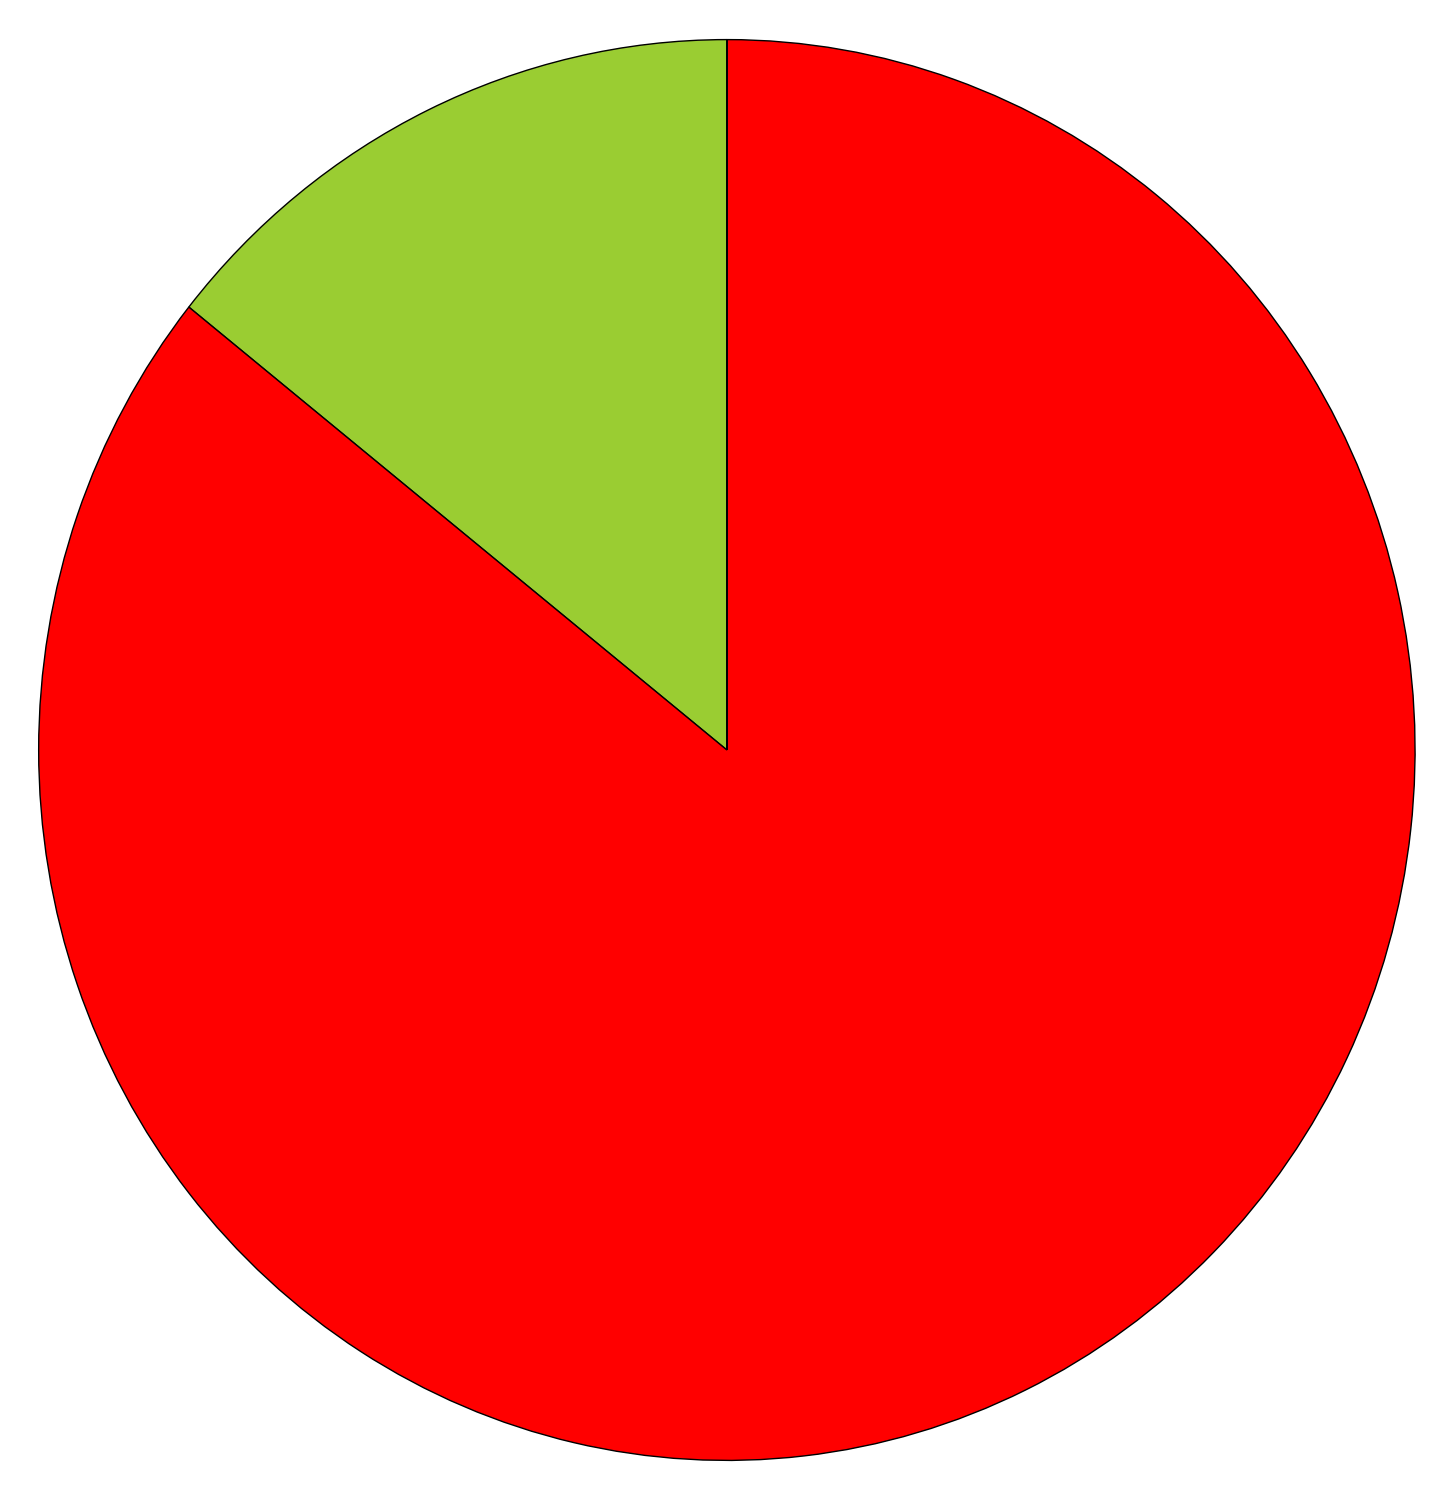
\includegraphics[width=\textwidth]{valenceALLSVMgen}
    \caption{SVM}
  \end{subfigure}
  
  \begin{subfigure}[b]{0.3\textwidth}
    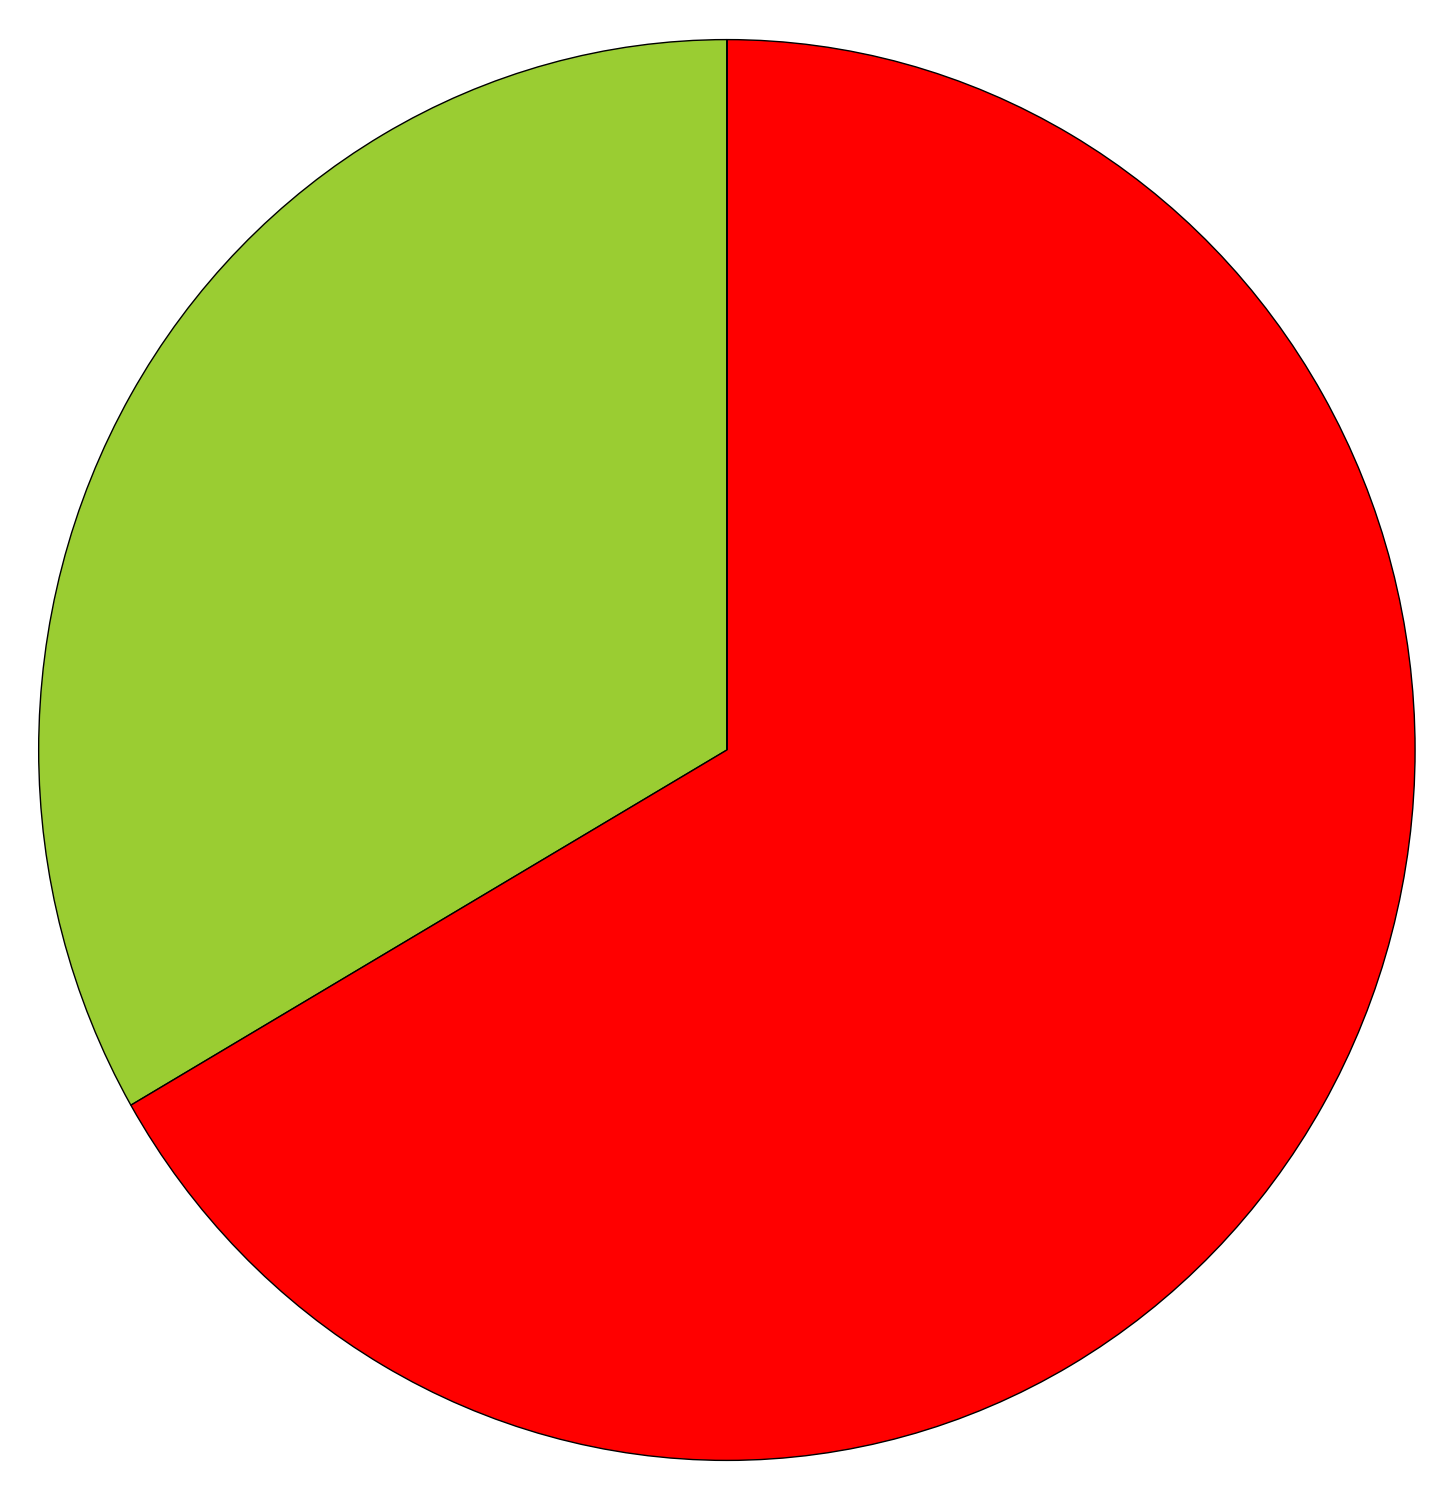
\includegraphics[width=\textwidth]{valenceALLLDAgen}
    \caption{LDA}
  \end{subfigure}
  \hfill
  \begin{subfigure}[b]{0.3\textwidth}
    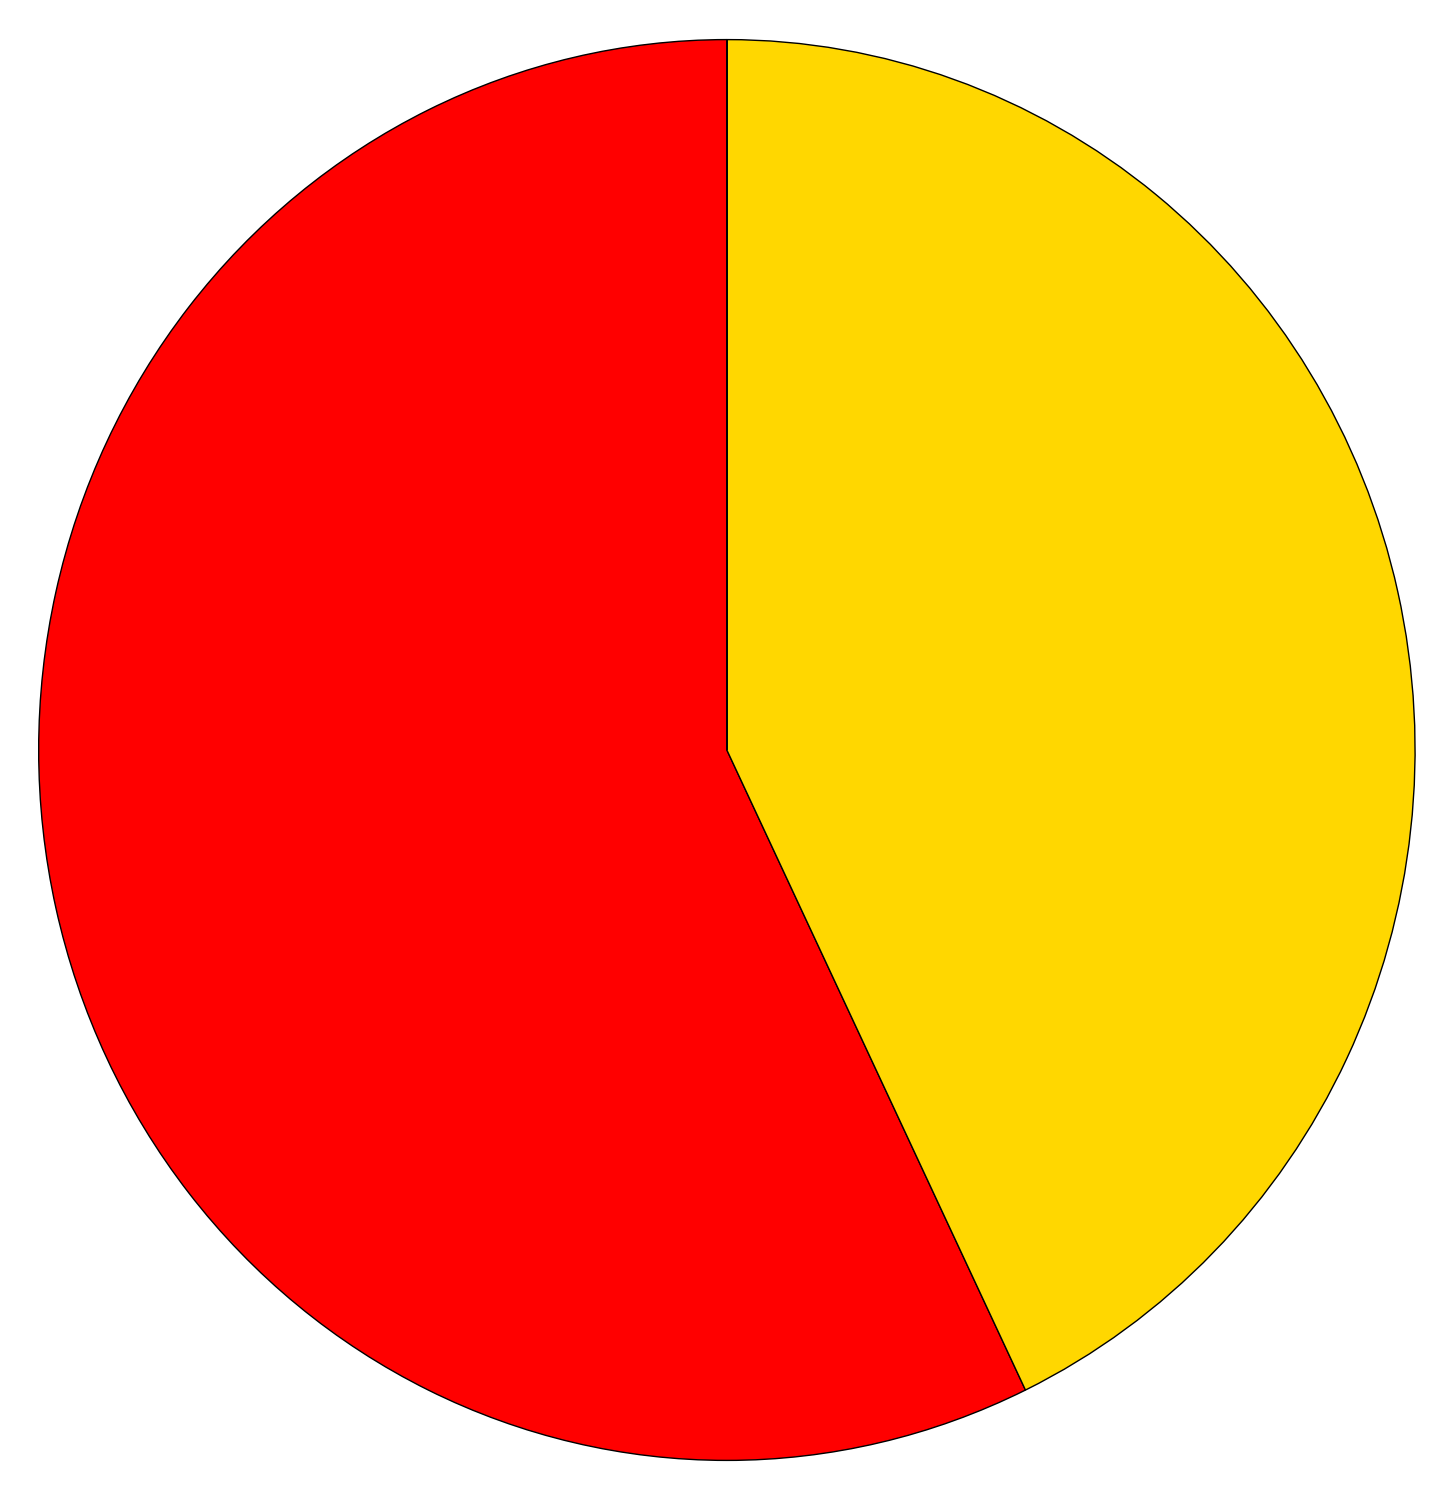
\includegraphics[width=\textwidth]{valenceALLL1gen}
    \caption{Lasso regression}
  \end{subfigure}
  \hfill
  \begin{subfigure}[b]{0.3\textwidth}
    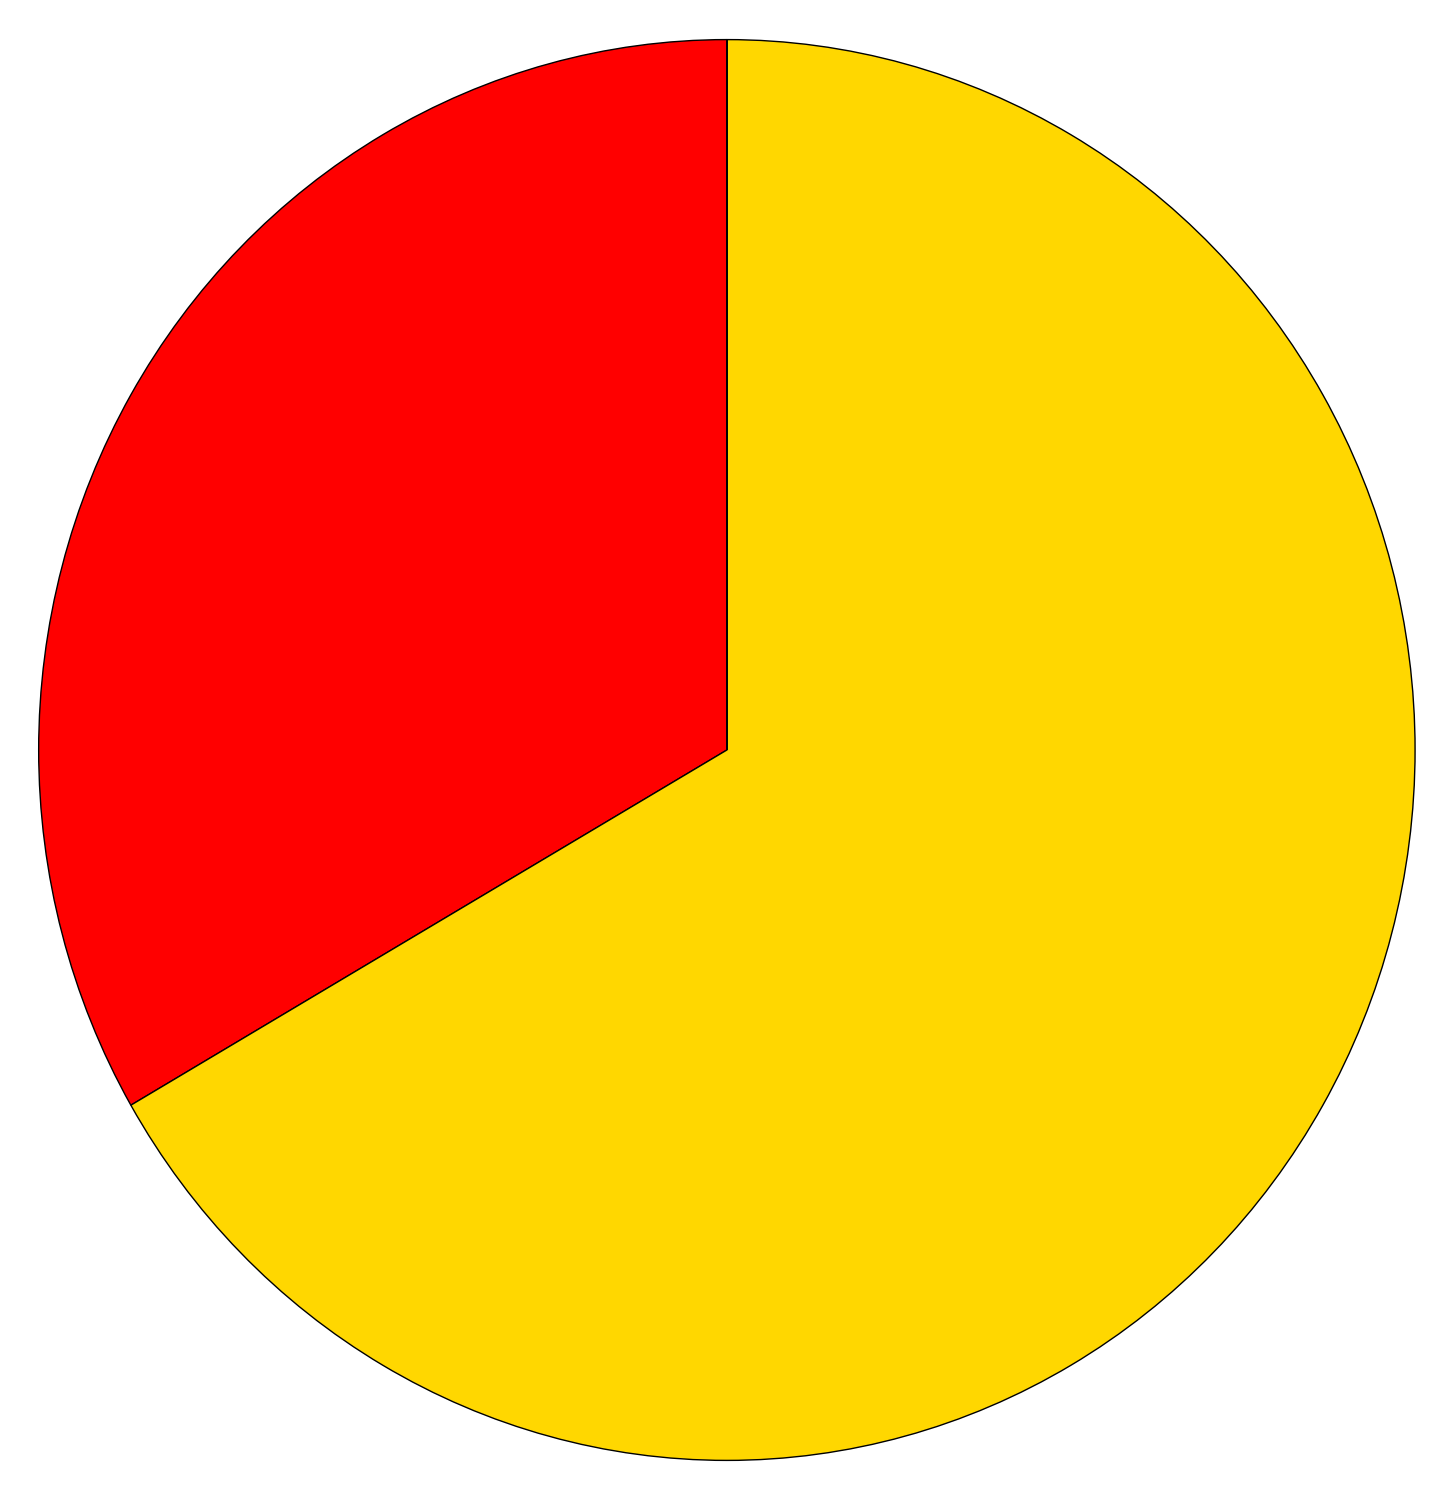
\includegraphics[width=\textwidth]{valenceALLL2gen}
    \caption{Ridge regression}
  \end{subfigure}
  
  \begin{subfigure}[b]{0.3\textwidth}
    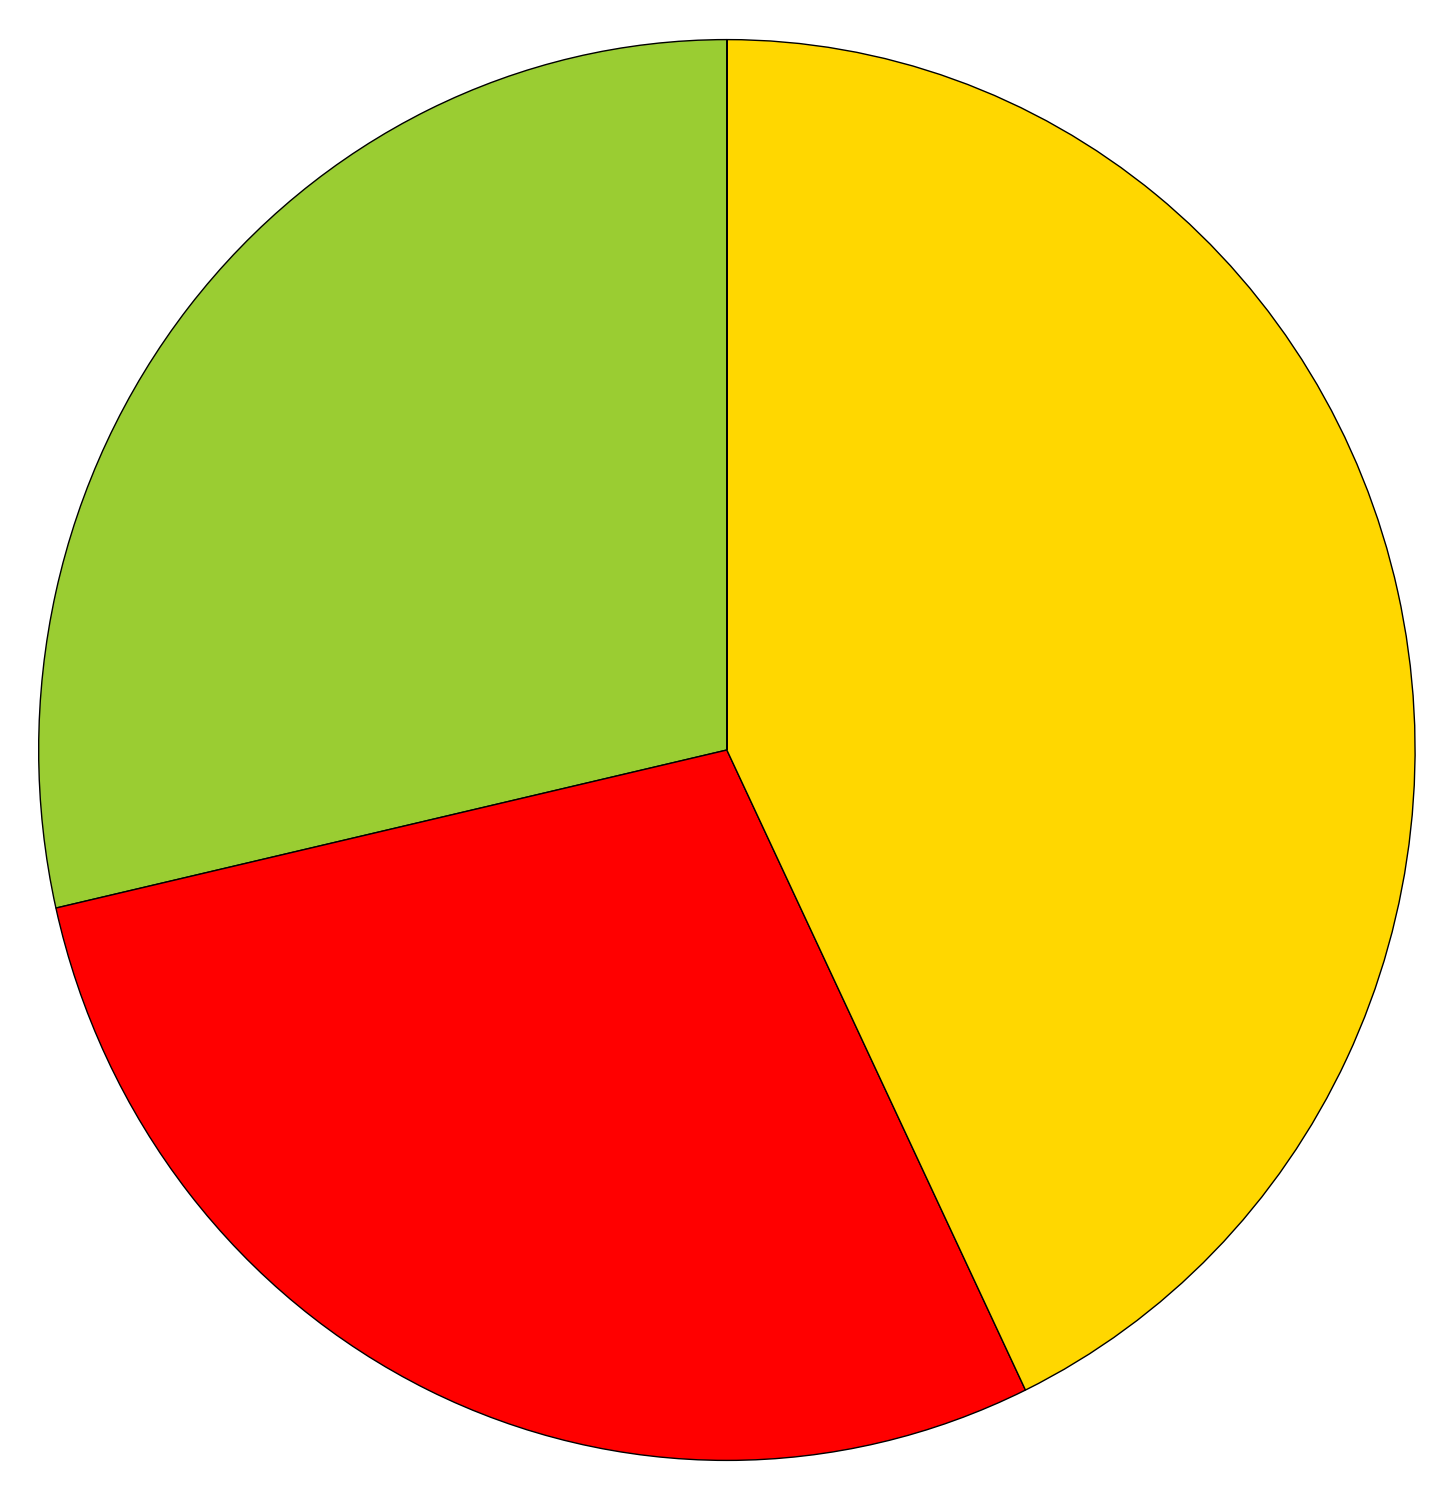
\includegraphics[width=\textwidth]{valenceALLRFgen}
    \caption{Random forests}
  \end{subfigure}
  \hfill
  \begin{subfigure}[b]{0.3\textwidth}
    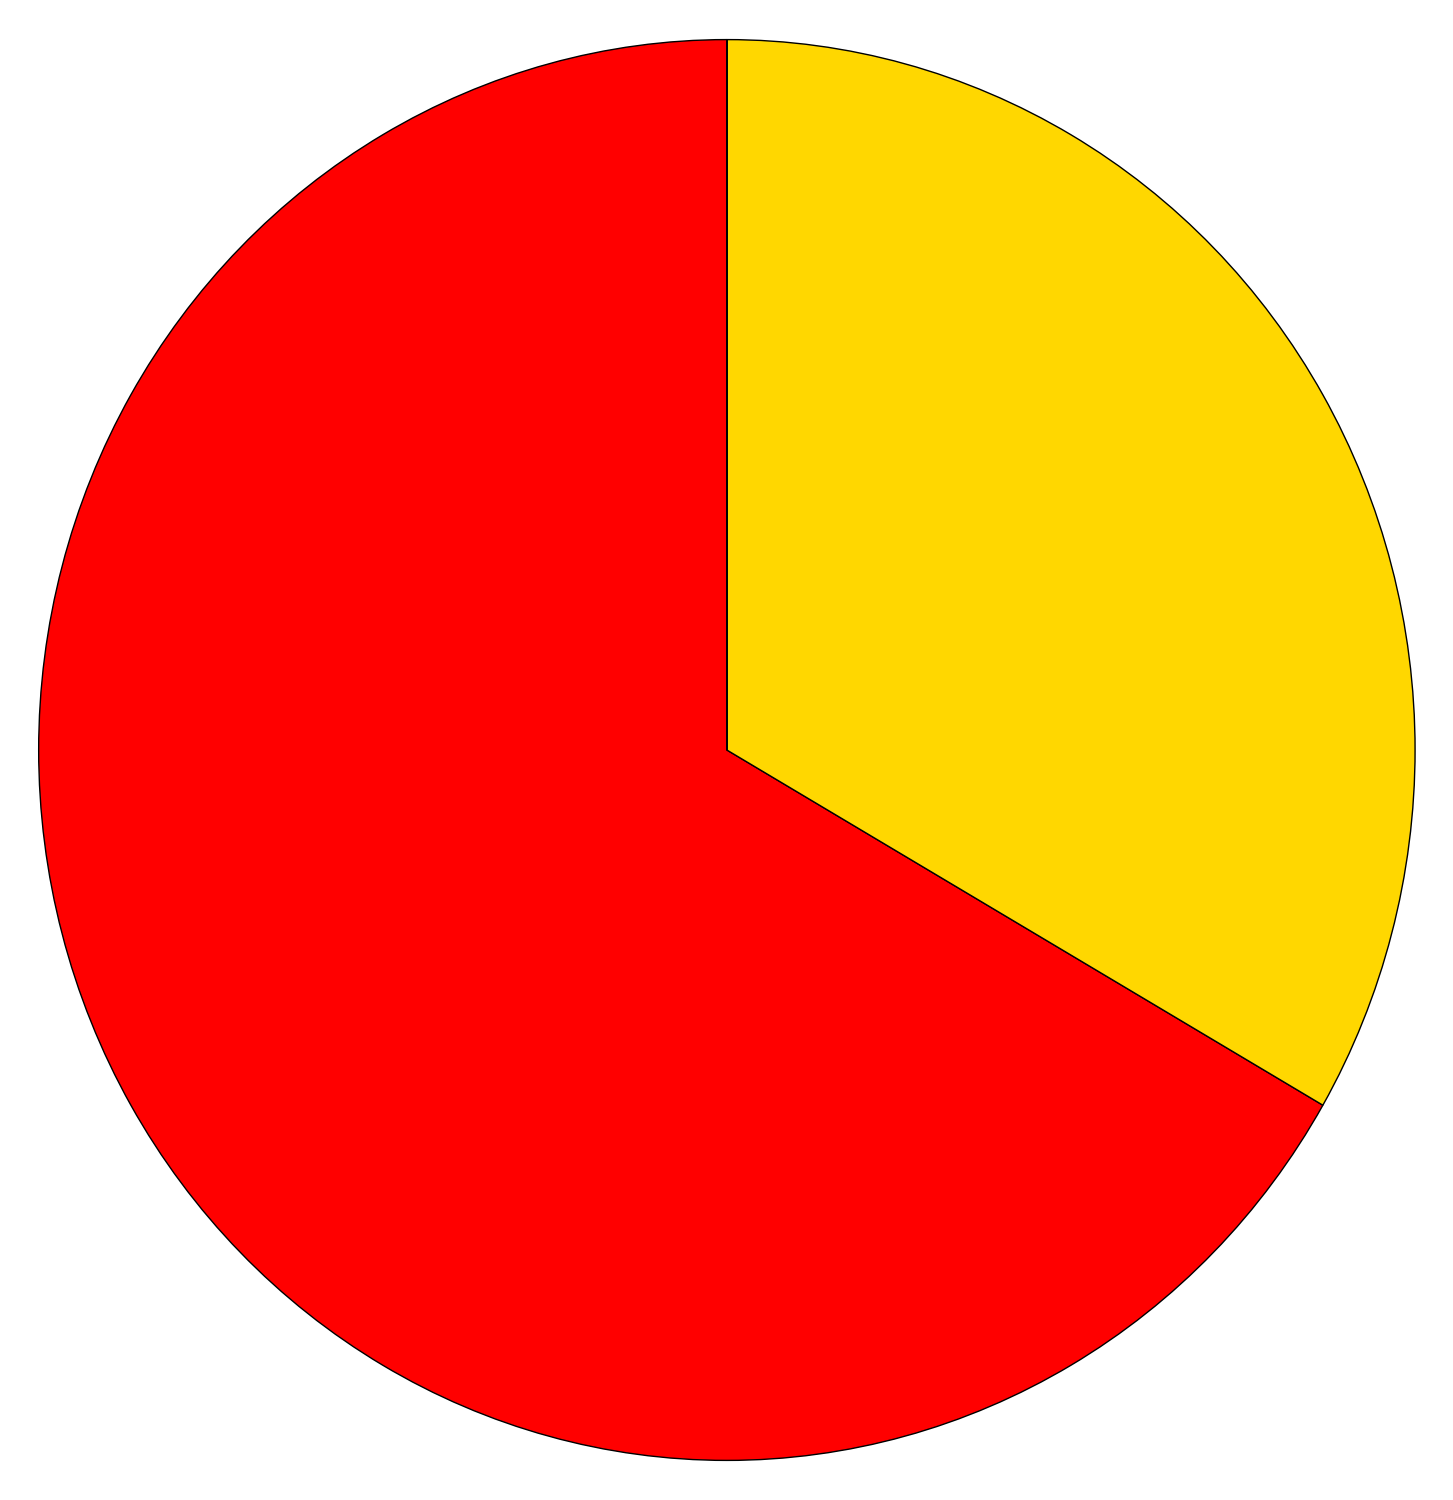
\includegraphics[width=\textwidth]{valenceALLPCAgen}
    \caption{PCA}
  \end{subfigure}
  \hfill
  \begin{subfigure}[b]{0.3\textwidth}
    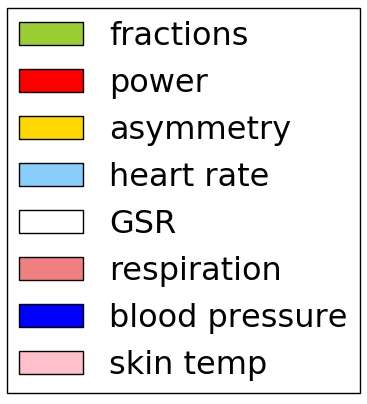
\includegraphics[width=\textwidth]{legend}
    \caption{Legend\label{valencepieslegendgen}}
  \end{subfigure}
\end{figure}
\clearpage

For arousal, it is clear that the EEG features are quite dominant. None the non-EEG features were selected. The EEG features themselves differ from selection method to selection method. One possible explanation for this is that the accuracies of the models are not great. The models are thus not fitting very well. This may cause unstable behaviour. The random forest method is the most advanced feature selection method and it gives a small preference to asymmetry features. This concurs with the person specific findings.

\npar

Similar things can be observed for valence. Again, the asymmetry features are preferred by the random forest, which concurs with similar studies. It might be important to note that there is a high correlation between asymmetry and the valence, which is visible when looking at the Pearson correlation output.

\npar

To further look at the difference between EEG and non-EEG features, the random forest selection method was again used three times. The first time, all features were available. The second and third time, only EEG and non-EEG features were available respectively. The results are shown in Figure \ref{arousalphyeegall_gen}, for arousal and Figure \ref{valencephyeegall_gen} for valence. The exact values are shown in Table \ref{phyeegallgenTable}.


\mijnfiguur{width=1.\textwidth}{arousalphyeegall_gen}{The performance of arousal prediction for all, EEG and non-EEG features in a cross-person setting.}

\mijnfiguur{width=1.\textwidth}{valencephyeegall_gen}{The performance of valence prediction for all, EEG and non-EEG features in a cross-person setting.}

\begin{table}[H]
\centering
\caption{The test accuracies for both arousal and valence, using different feature sets.\label{phyeegallgenTable}}
\begin{tabular}{l|ll}
\textbf{Feat set}  & \textbf{Avg acc - arousal}       & \textbf{Avg acc - valence}          \\ \hline
\textbf{All}       & 0.6344           & 0.5531           \\
\textbf{EEG}       & 0.6094           & 0.5656           \\
\textbf{non-EEG}   & 0.6344           & 0.5531          
\end{tabular}
\end{table}

Comparing Table \ref{phyeegallgenTable} with Table \ref{phyeegalltable}, one can see that the difference in accuracy between non-EEG features and all and/or EEG features only is much smaller. This is an indication that the non-EEG features might work better in a cross-person setting. The reason that the feature selection methods select only EEG features might be due to the fact there are more EEG features available. Given that EEG features often contain a lot of noise, chances are that the selection methods are able to find EEG features that fit the limit sample set well. 

\npar

To find out which non-EEG feature might be useful, the selected non-EEG features from the random forest selection method were analysed. The resulting model of each feature selection method is quite different. The random forest seems to prefer skin temperature, heart rate and GSR for arousal and blood pressure combined with GSR for valence.

\clearpage

\begin{figure}[!tbp]
  \centering
  \caption{Selection features for arousal classification, using only non-EEG features in a cross-person setting.\label{arousalnon-EEGpiesgen}}
  \begin{subfigure}[b]{0.3\textwidth}
    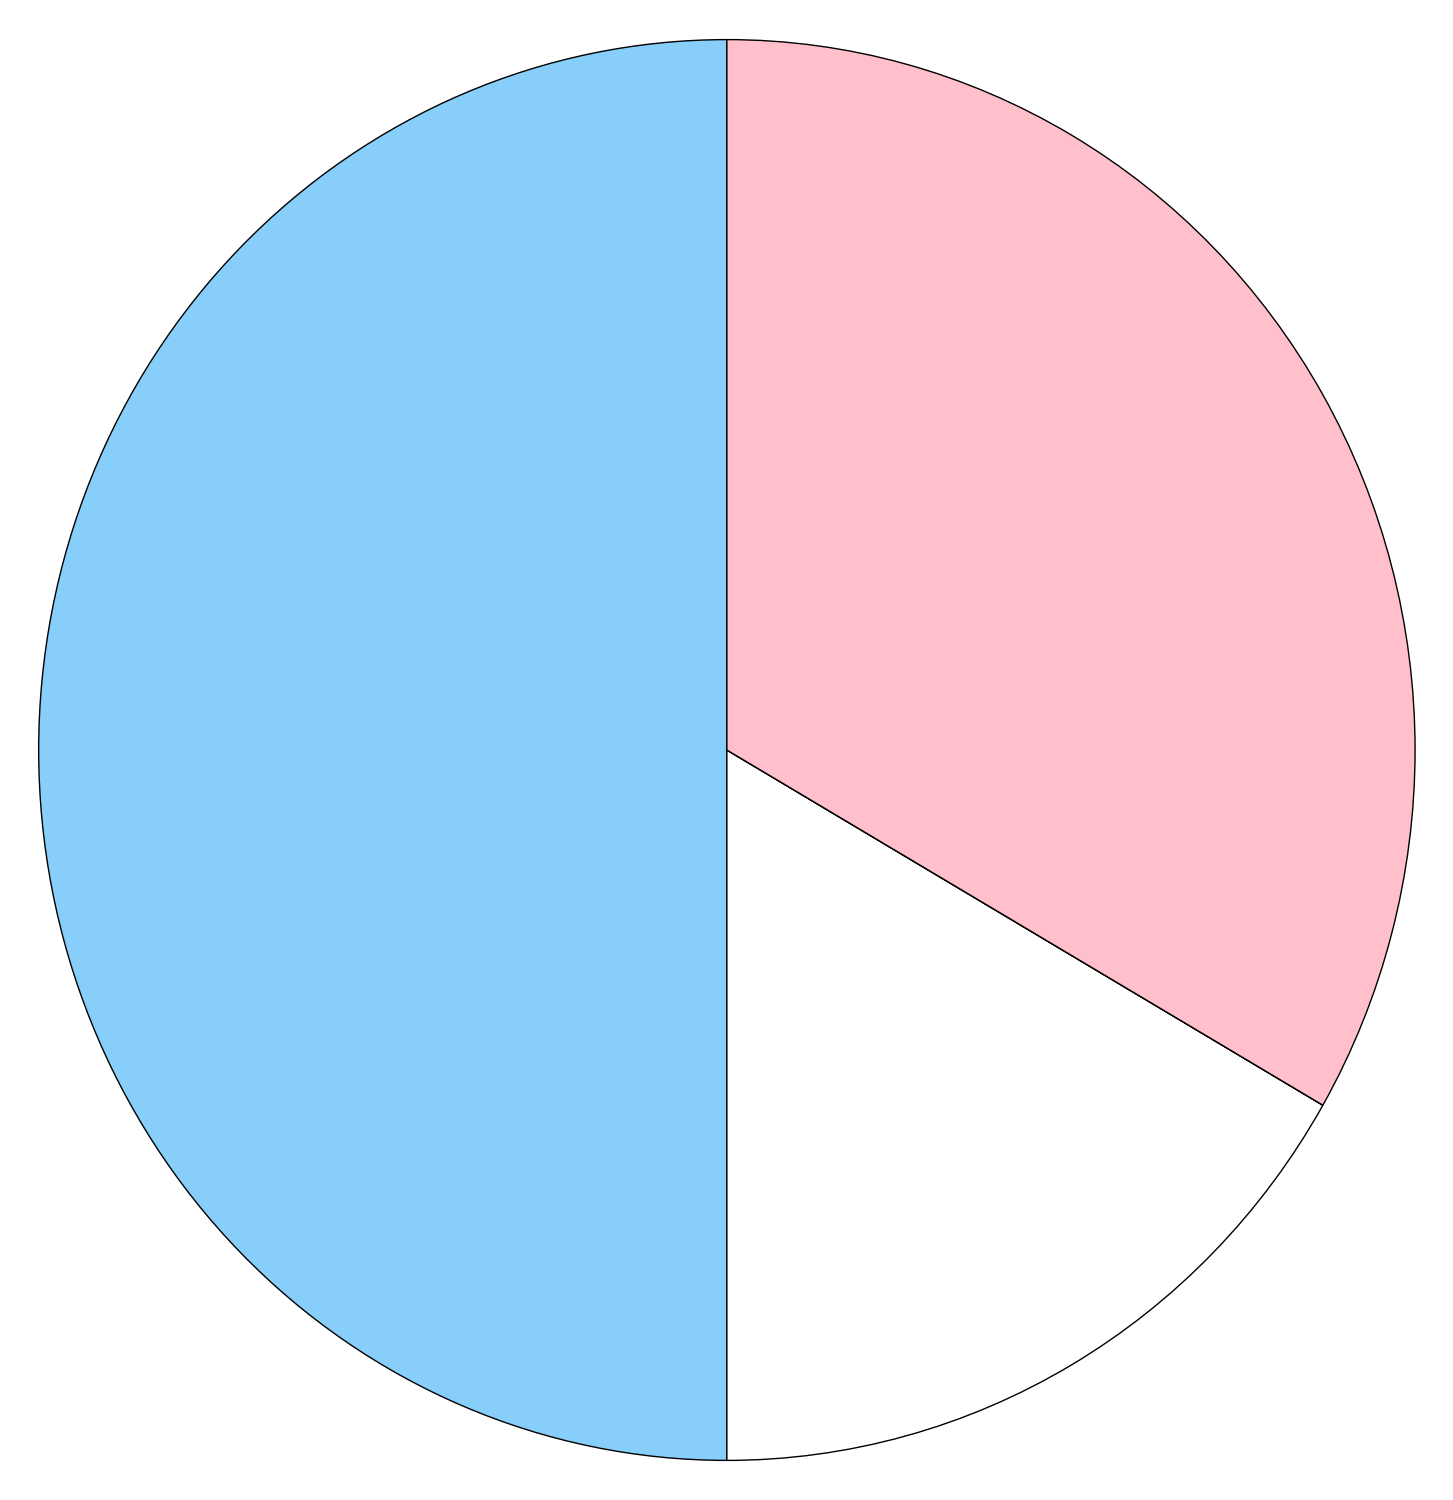
\includegraphics[width=\textwidth]{arousalnon-EEGpearsonRgen}
    \caption{Pearson correlation}
  \end{subfigure}
  \hfill
  \begin{subfigure}[b]{0.3\textwidth}
    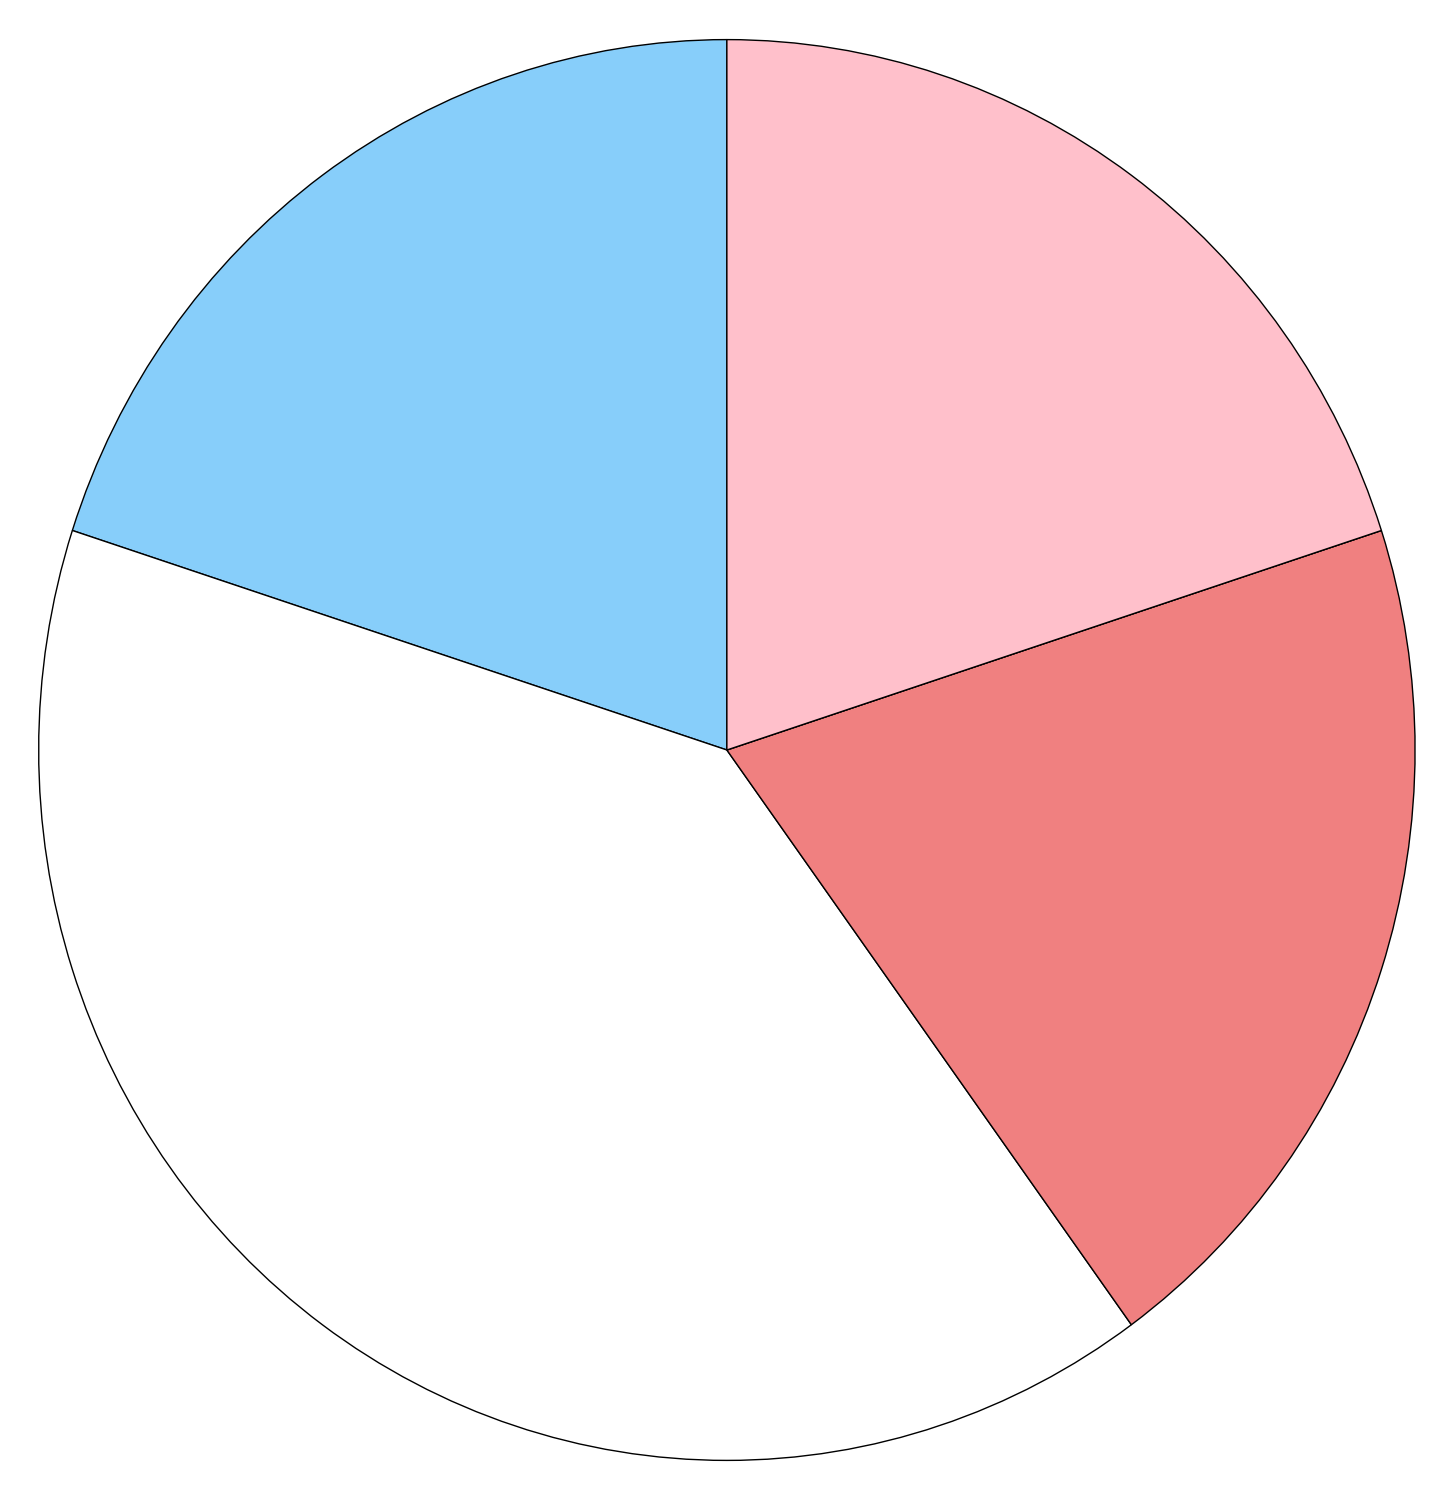
\includegraphics[width=\textwidth]{arousalnon-EEGMutInfgen}
    \caption{Mutual information}
  \end{subfigure}
  \hfill
  \begin{subfigure}[b]{0.3\textwidth}
    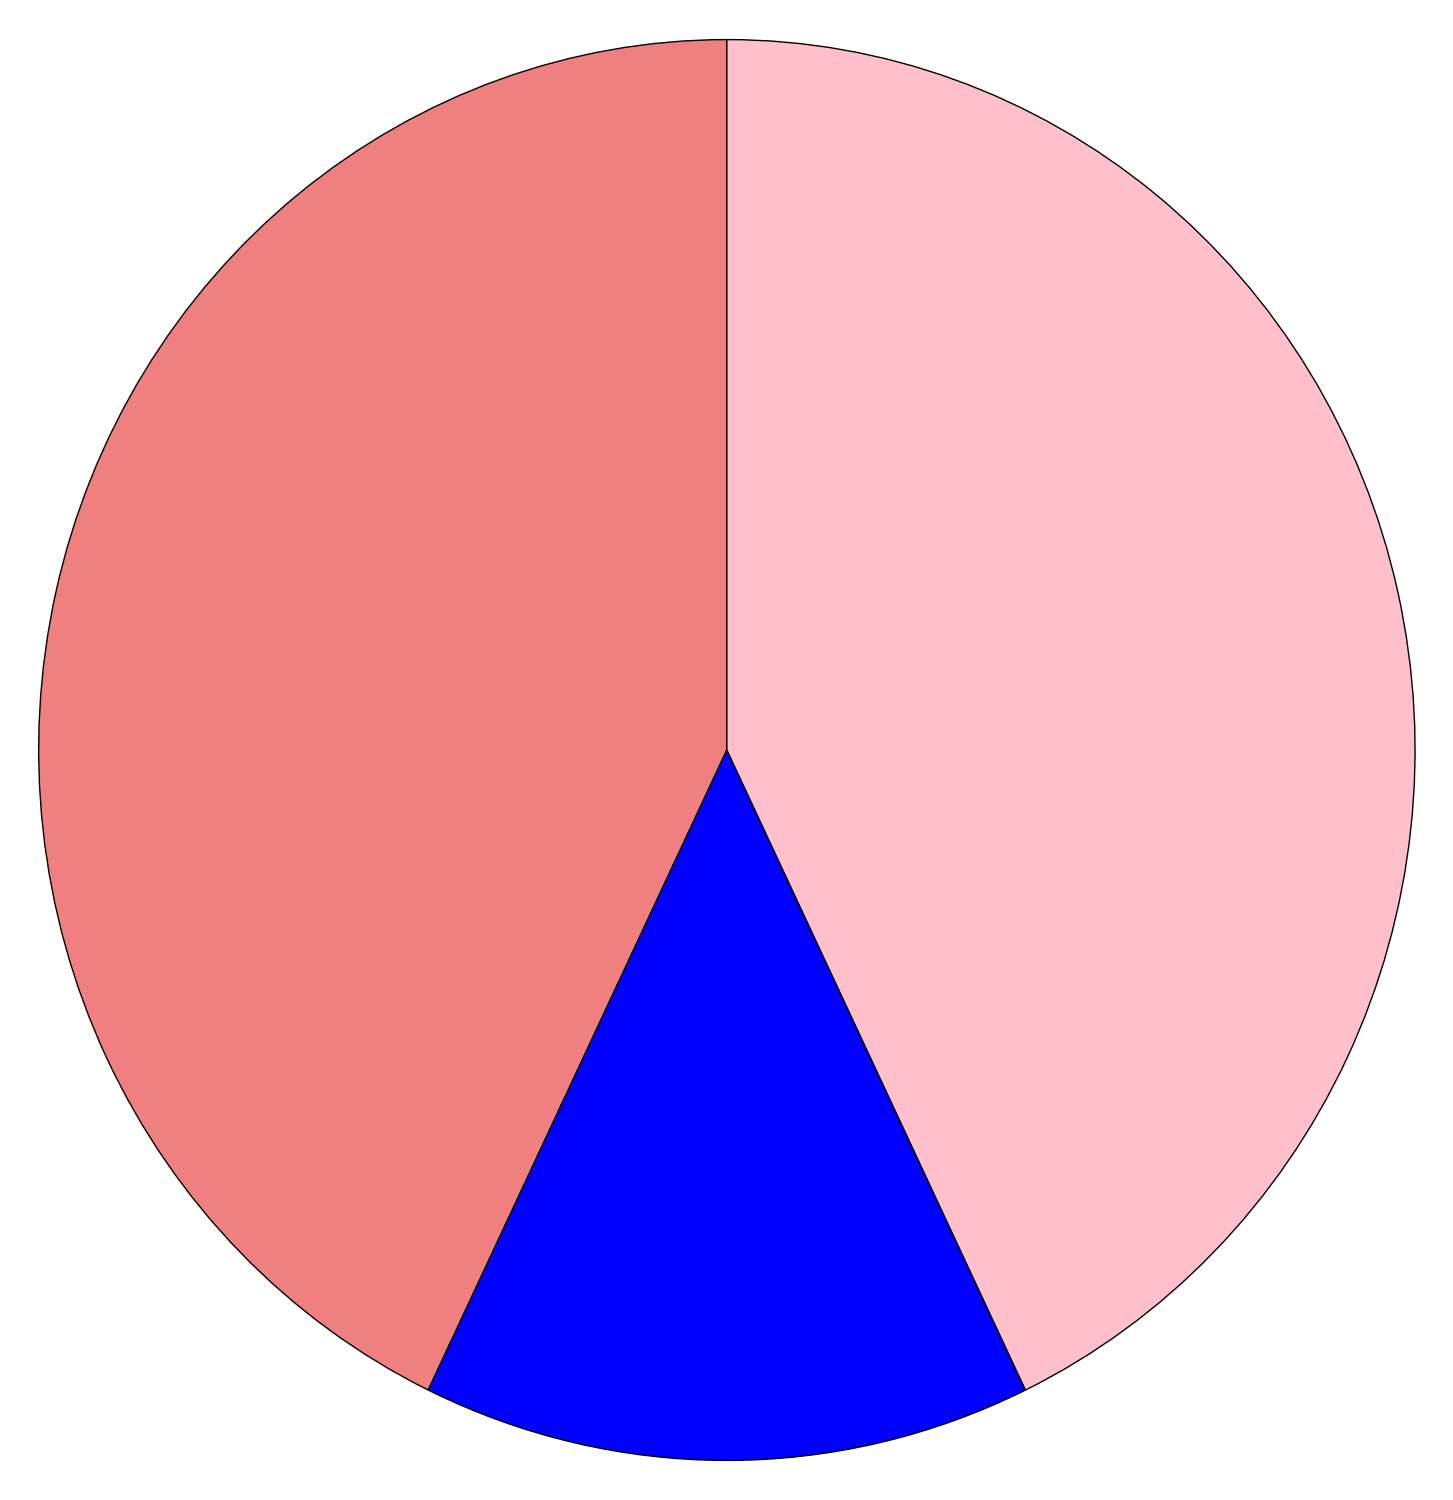
\includegraphics[width=\textwidth]{arousalnon-EEGdCorrgen}
    \caption{Distance Correlation}
  \end{subfigure}
  
  \begin{subfigure}[b]{0.3\textwidth}
    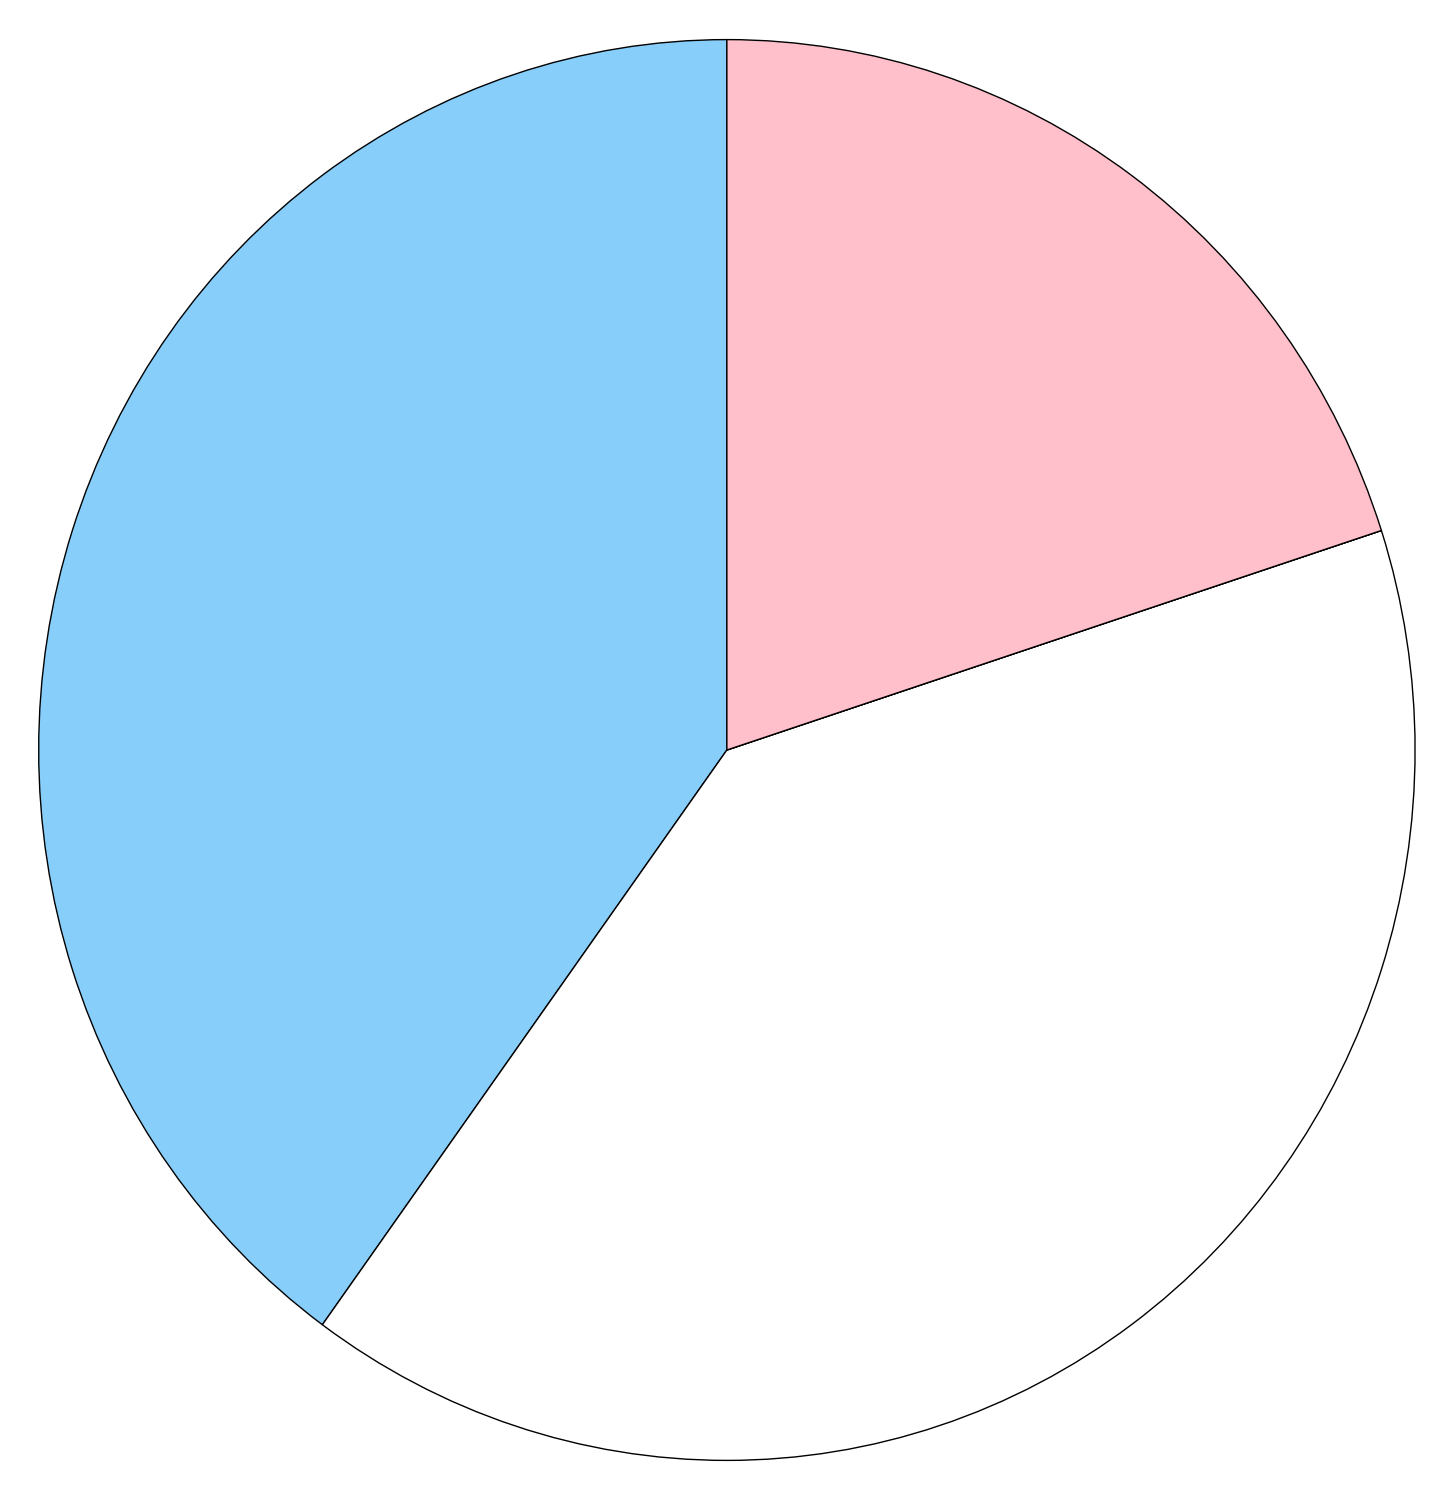
\includegraphics[width=\textwidth]{arousalnon-EEGANOVAgen}
    \caption{ANOVA}
  \end{subfigure}
  \hfill
  \begin{subfigure}[b]{0.3\textwidth}
    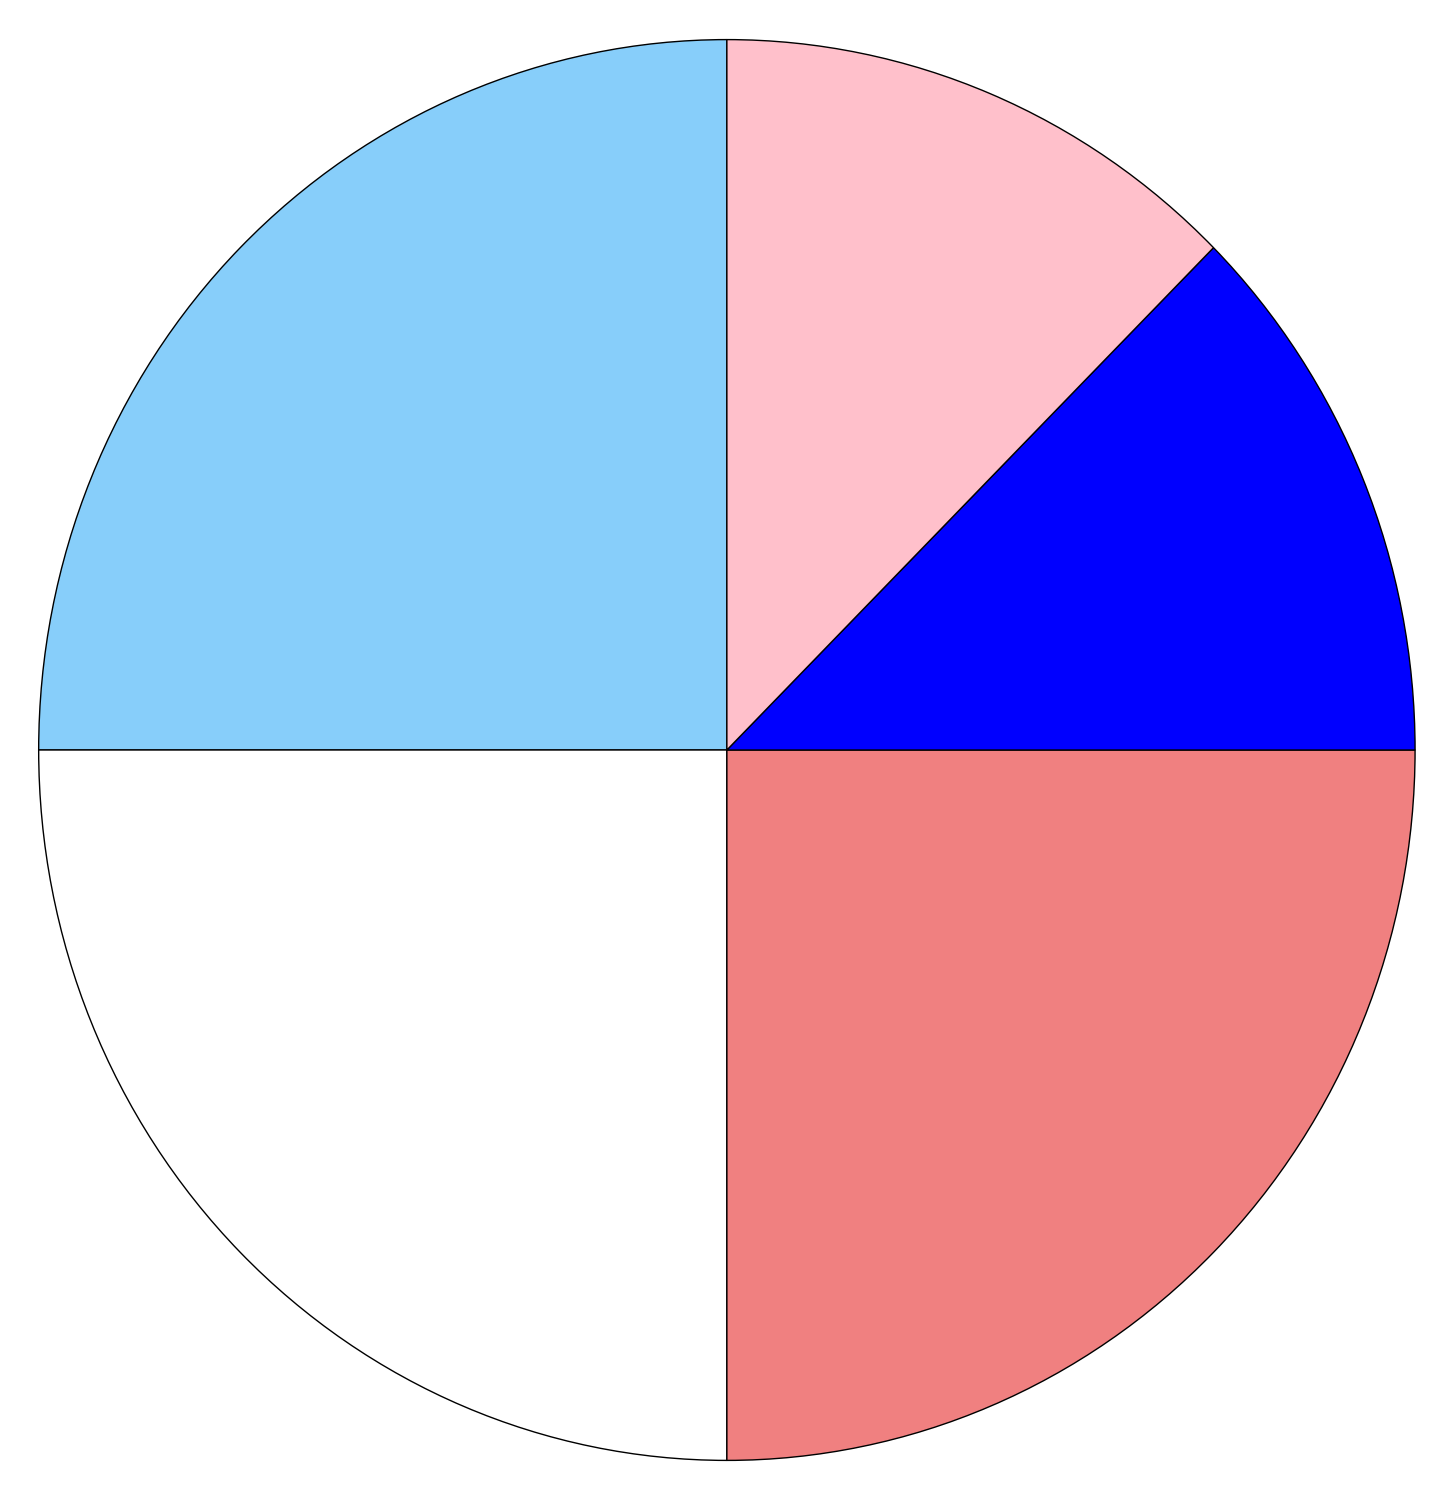
\includegraphics[width=\textwidth]{arousalnon-EEGLRgen}
    \caption{Linear regression}
  \end{subfigure}
  \hfill
  \begin{subfigure}[b]{0.3\textwidth}
    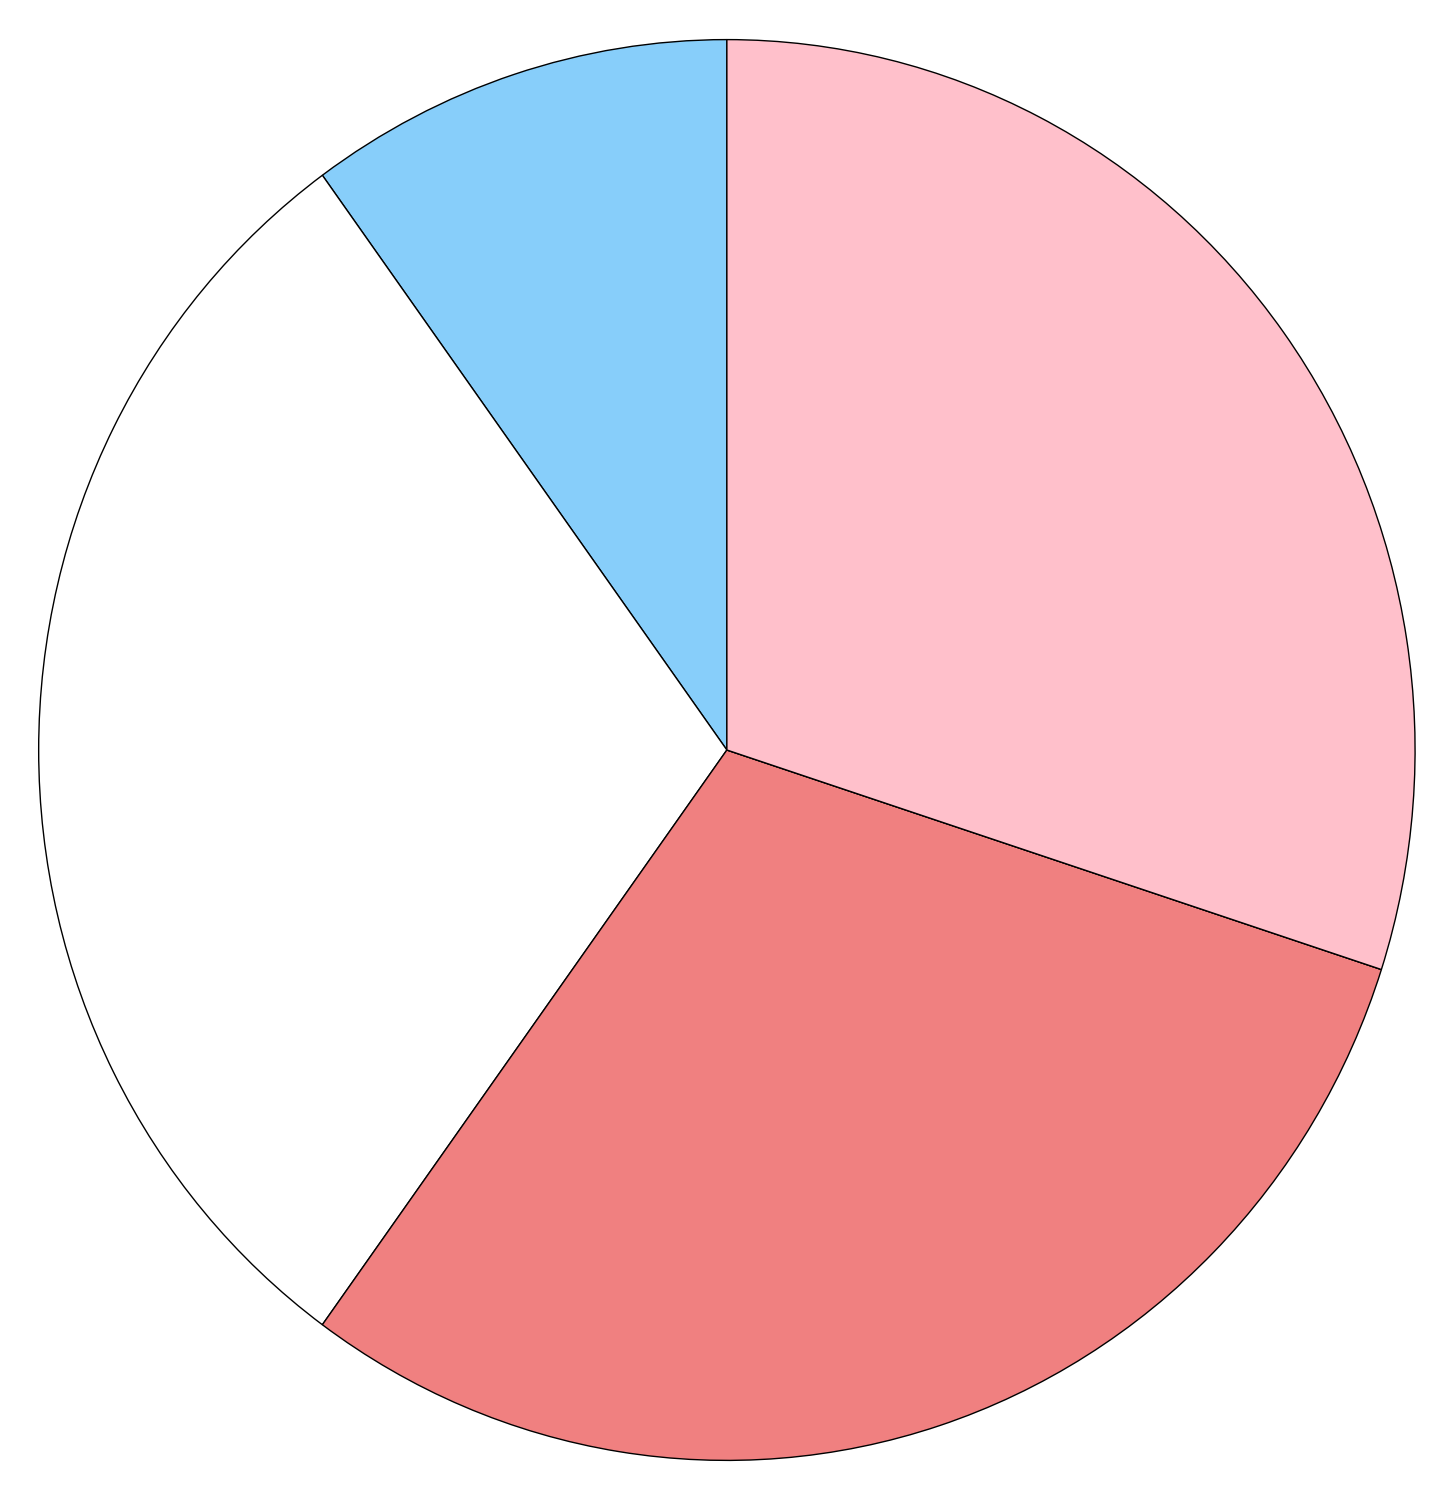
\includegraphics[width=\textwidth]{arousalnon-EEGSVMgen}
    \caption{SVM}
  \end{subfigure}
  
  \begin{subfigure}[b]{0.3\textwidth}
    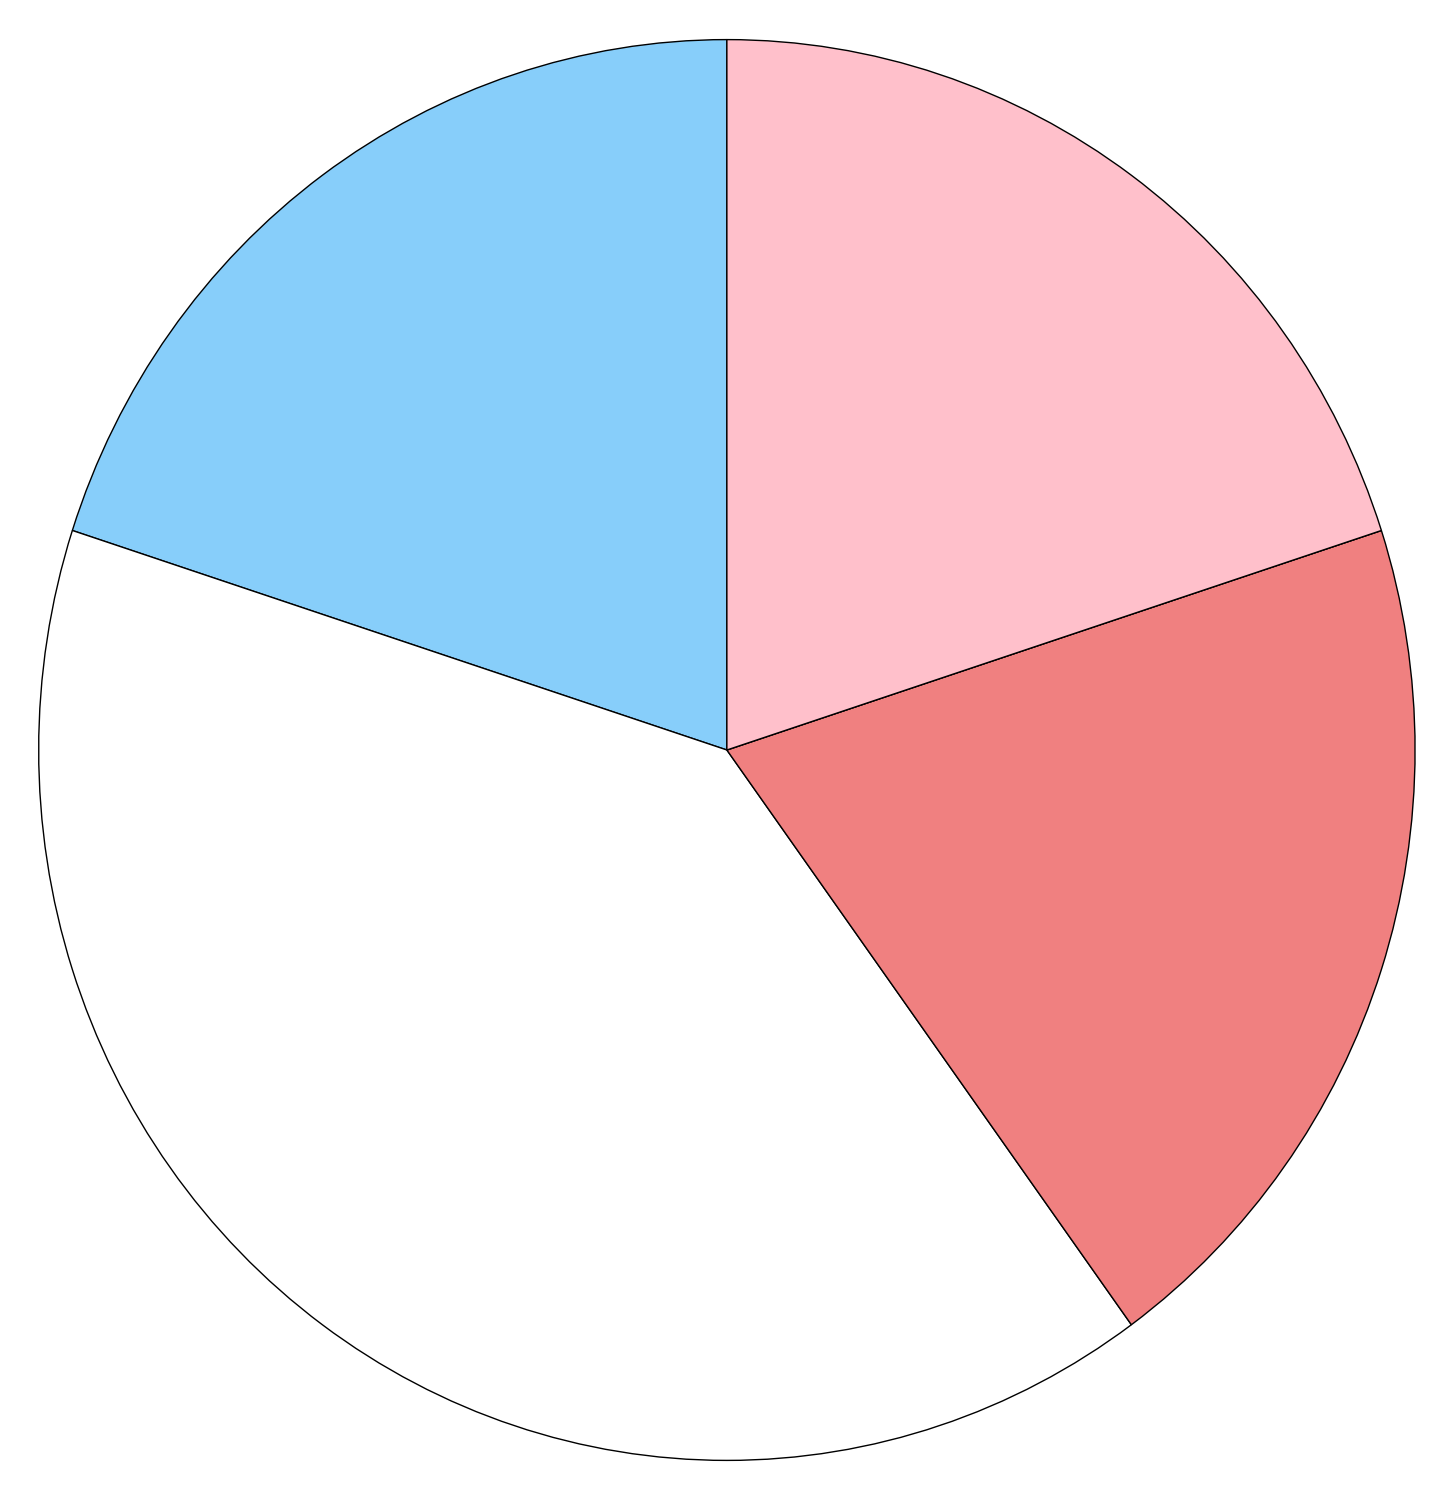
\includegraphics[width=\textwidth]{arousalnon-EEGLDAgen}
    \caption{LDA}
  \end{subfigure}
  \hfill
  \begin{subfigure}[b]{0.3\textwidth}
    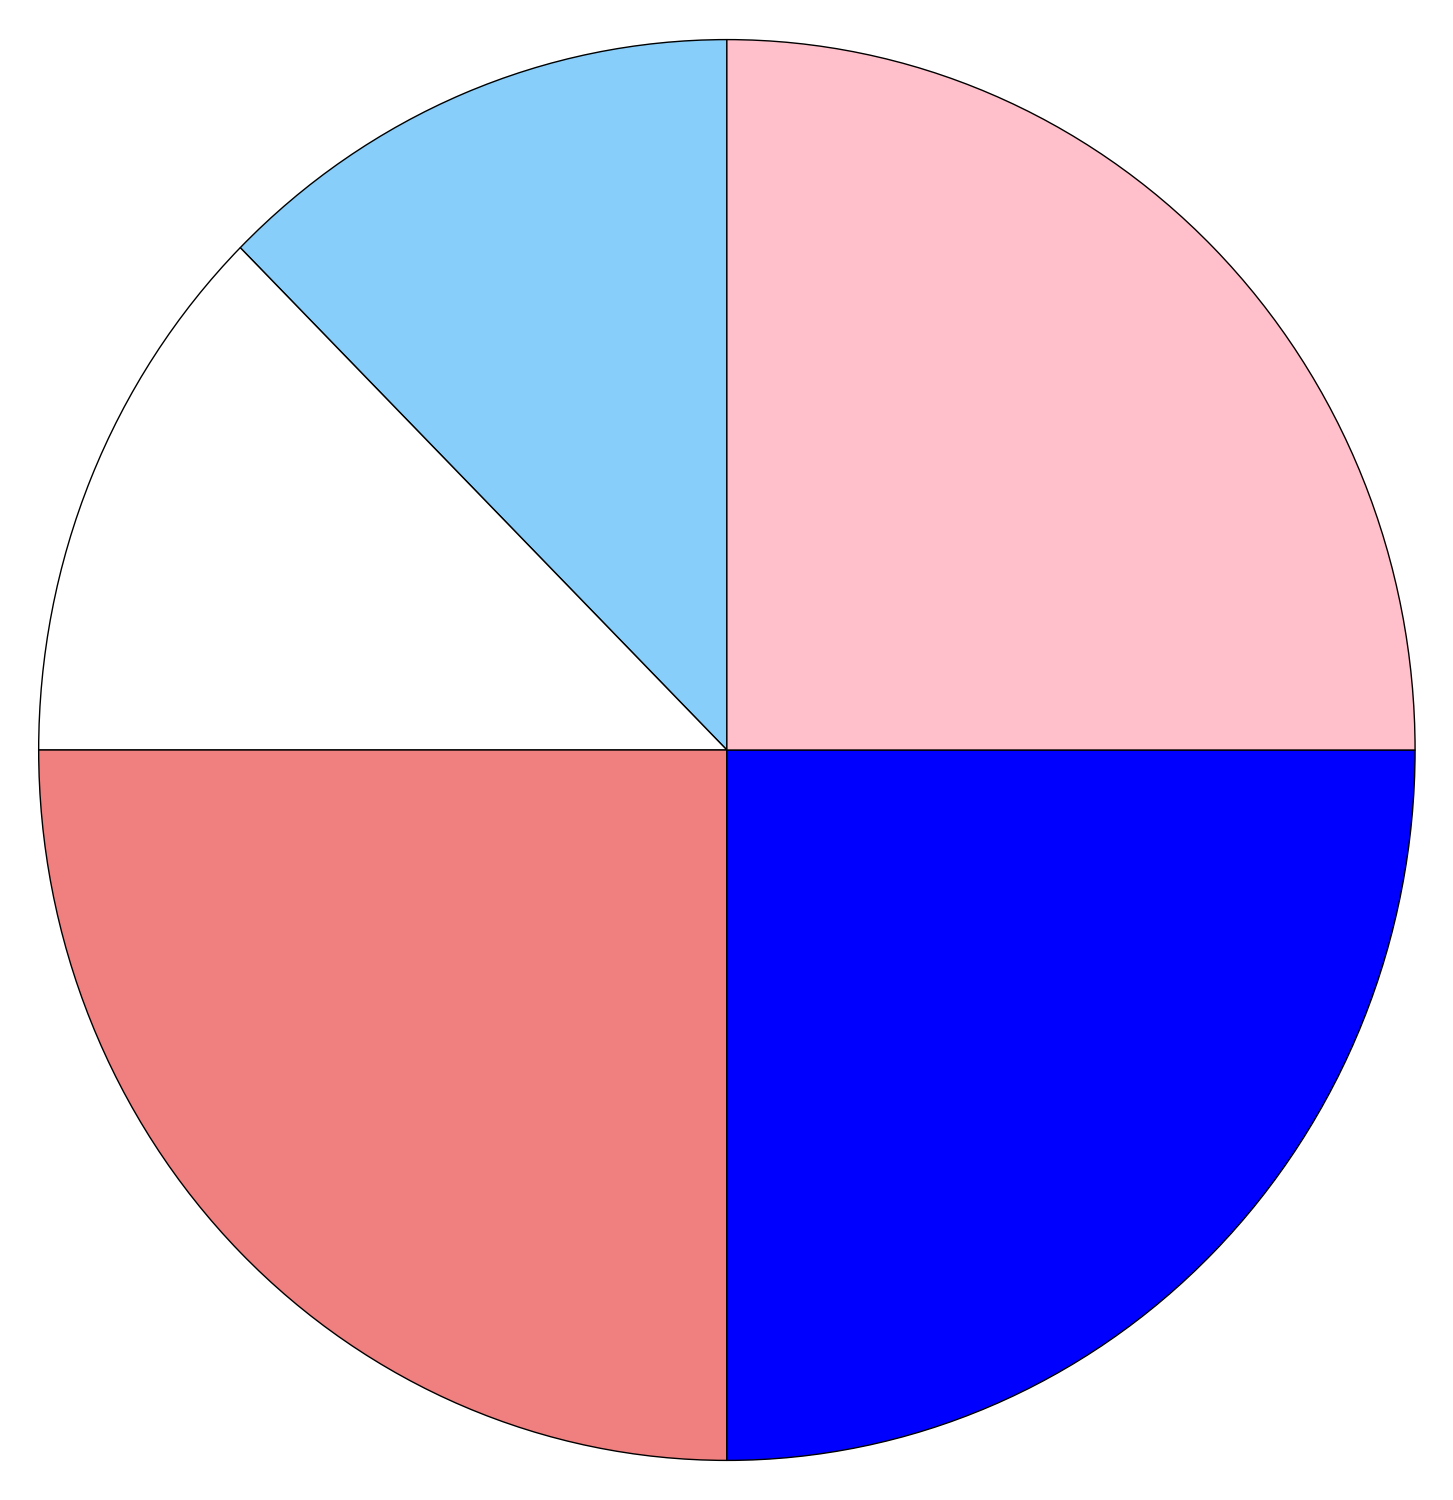
\includegraphics[width=\textwidth]{arousalnon-EEGL1gen}
    \caption{Lasso regression}
  \end{subfigure}
  \hfill
  \begin{subfigure}[b]{0.3\textwidth}
    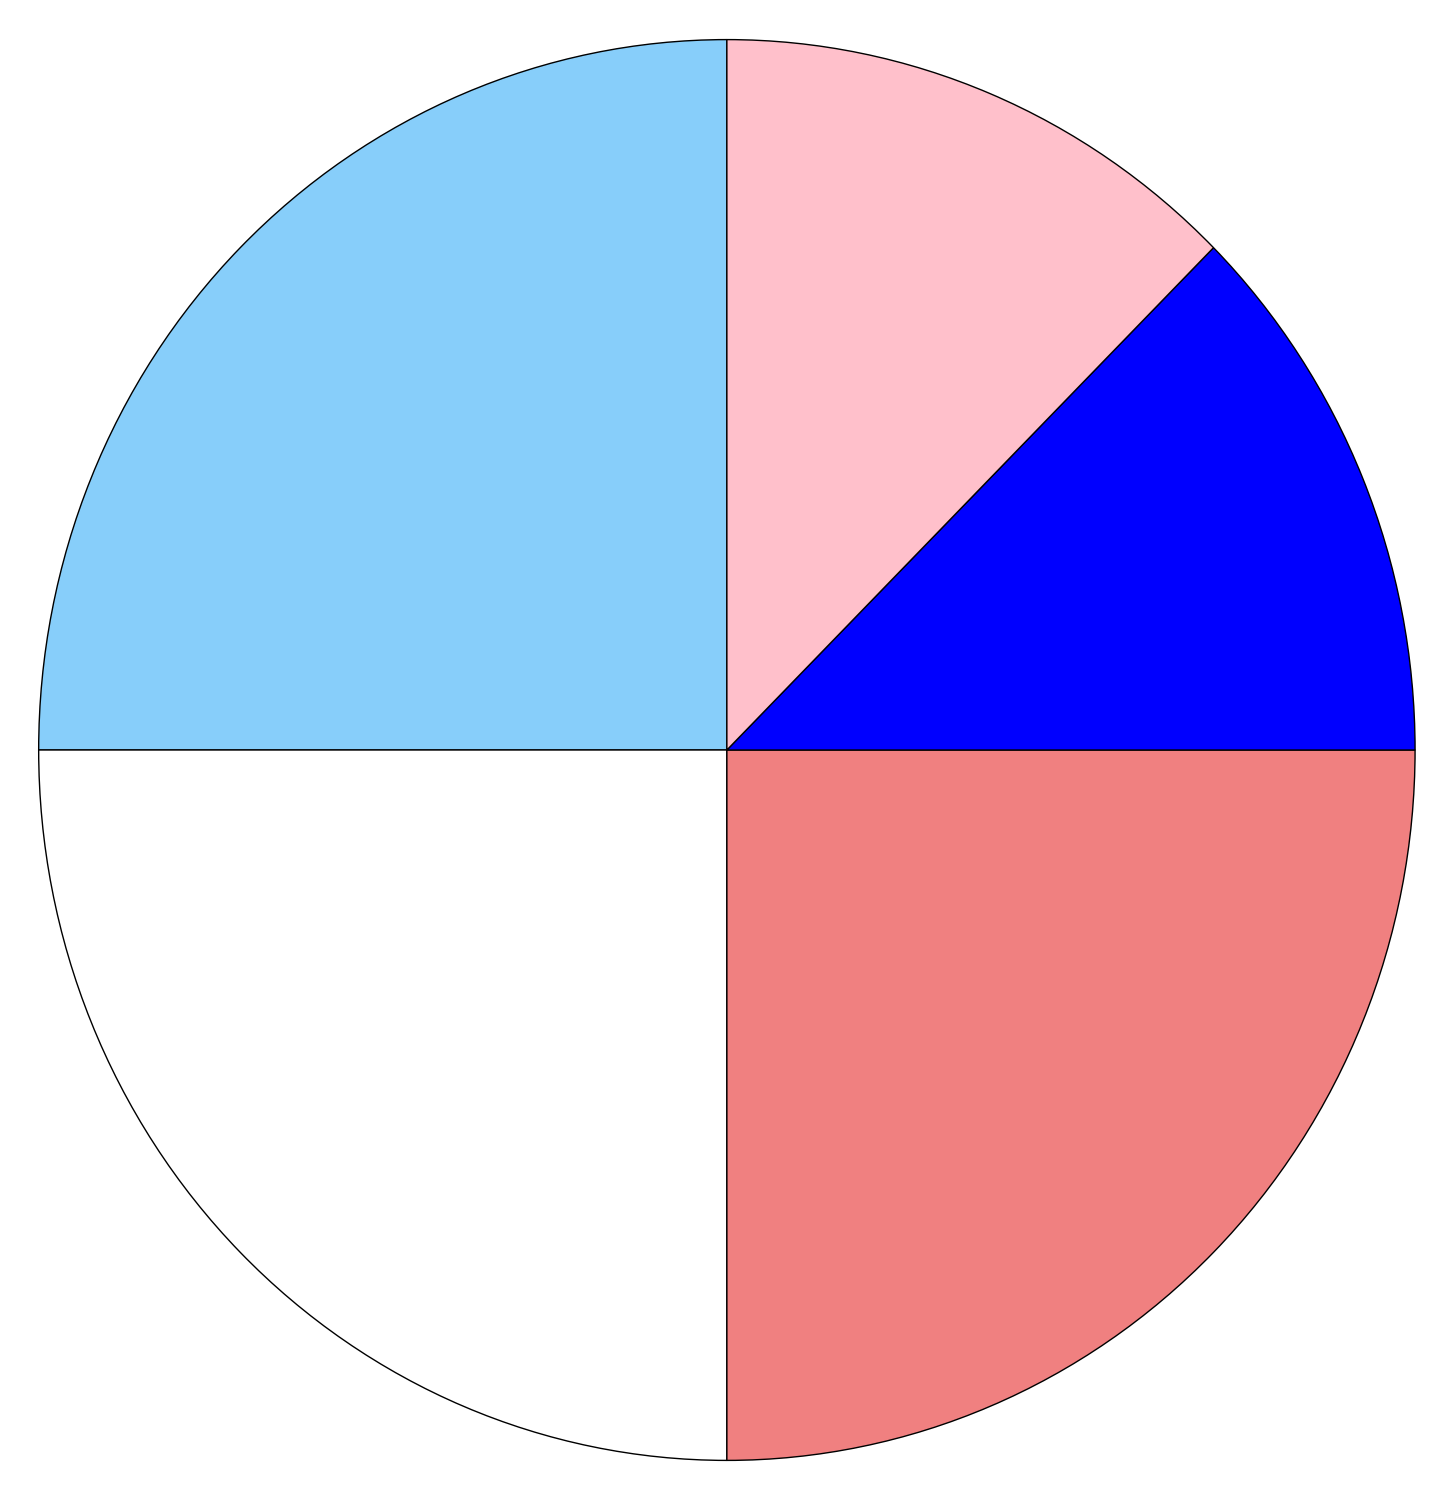
\includegraphics[width=\textwidth]{arousalnon-EEGL2gen}
    \caption{Ridge regression}
  \end{subfigure}
  
  \begin{subfigure}[b]{0.3\textwidth}
    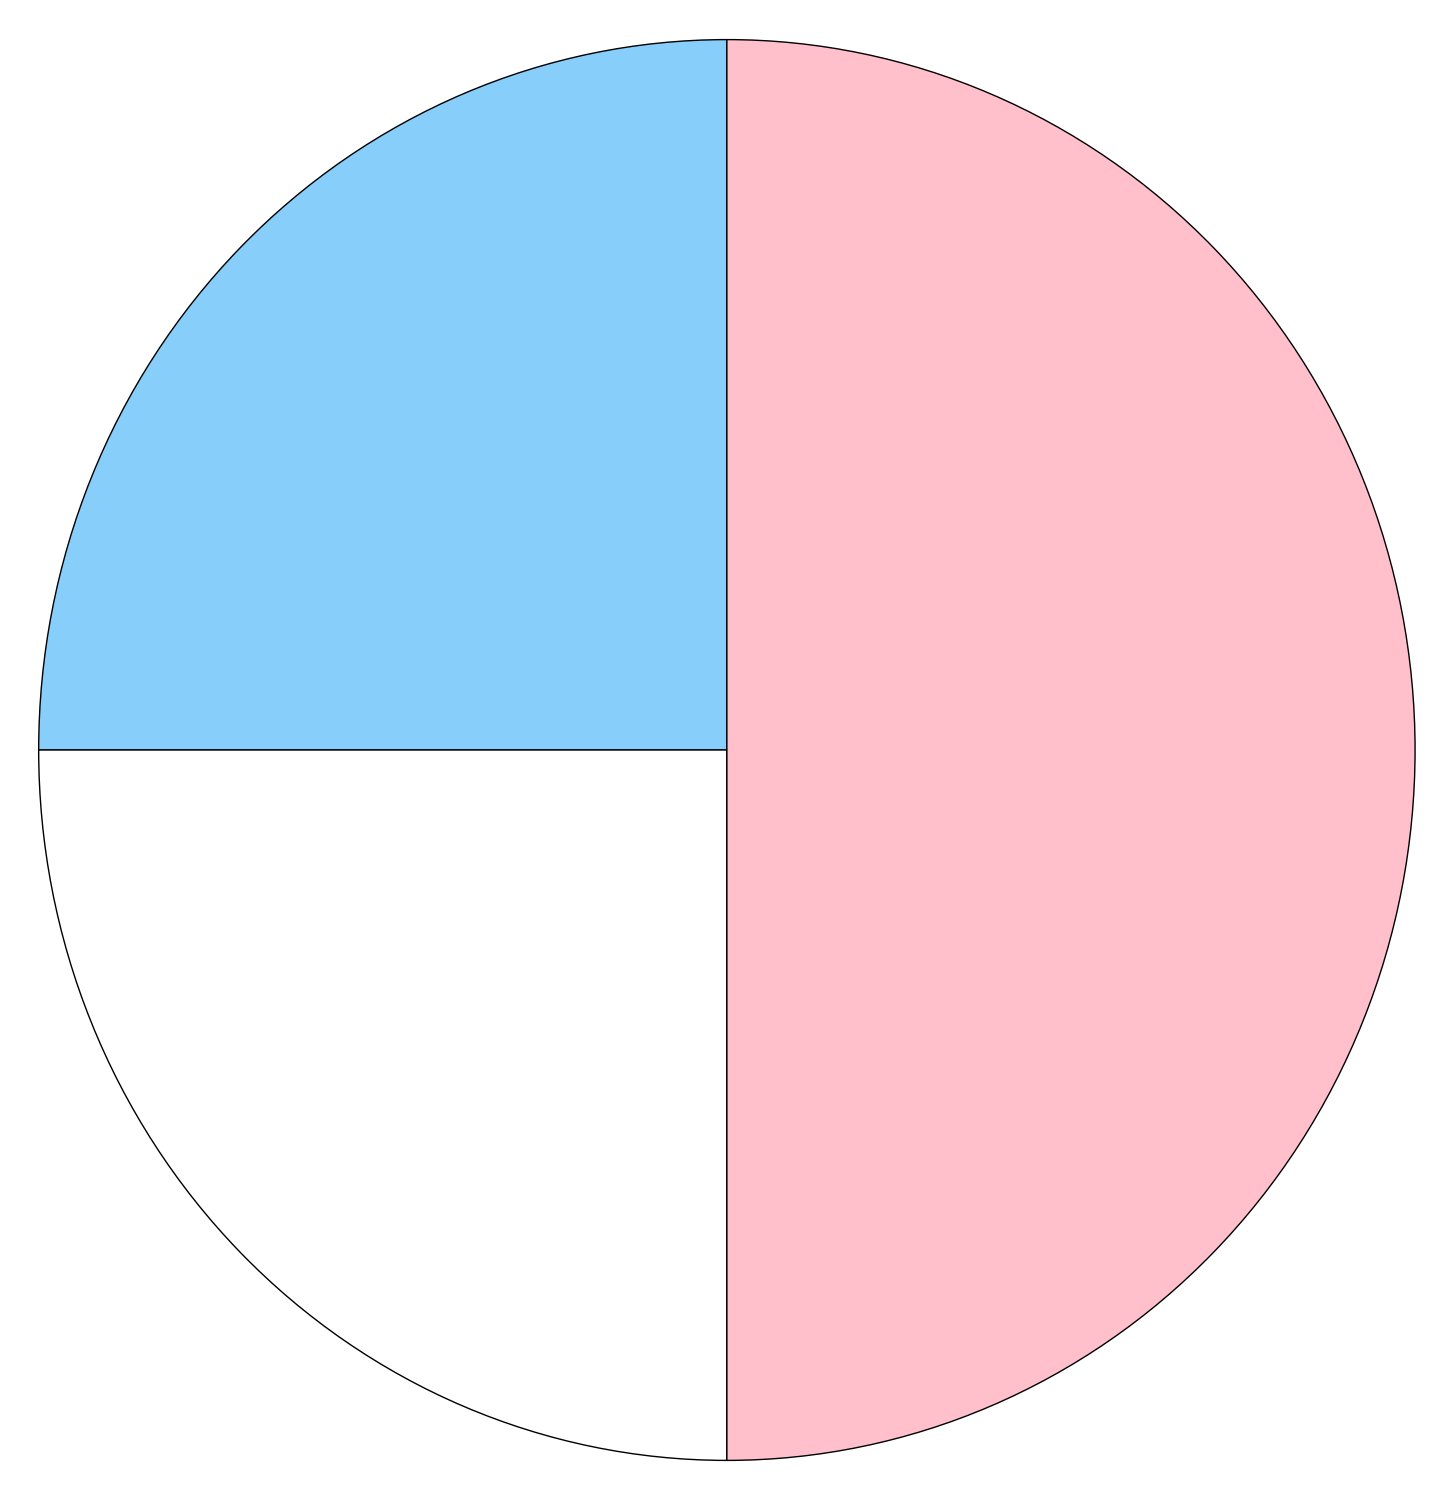
\includegraphics[width=\textwidth]{arousalnon-EEGRFgen}
    \caption{Random forests}
  \end{subfigure}
  \hfill
  \begin{subfigure}[b]{0.3\textwidth}
    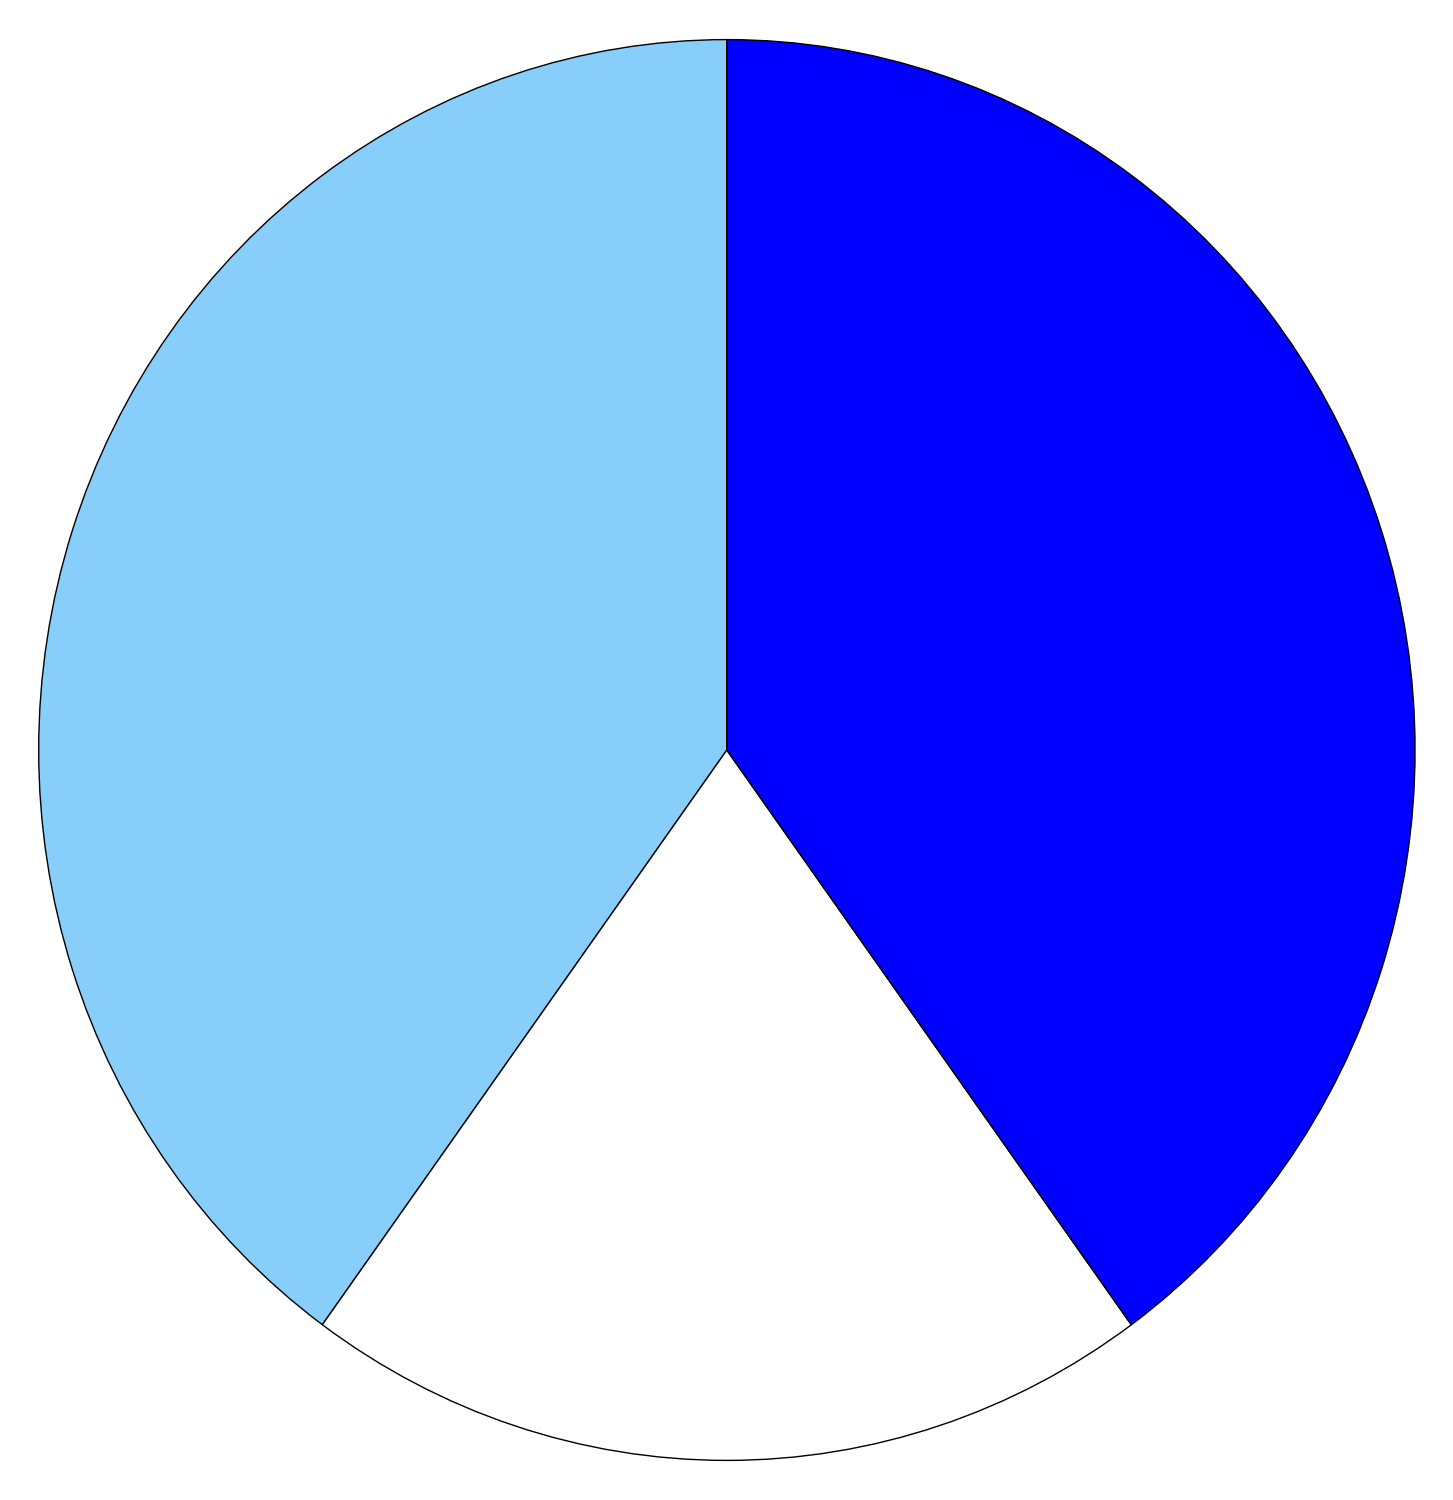
\includegraphics[width=\textwidth]{arousalnon-EEGPCAgen}
    \caption{PCA}
  \end{subfigure}
  \hfill
  \begin{subfigure}[b]{0.3\textwidth}
    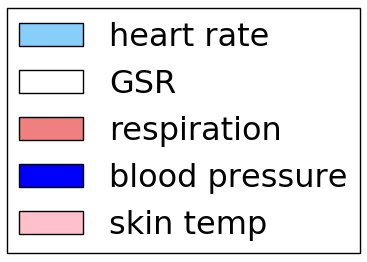
\includegraphics[width=\textwidth]{non-EEGlegend}
    \caption{Legend\label{arousalpiesnon-EEGlegendgen}}
  \end{subfigure}
\end{figure}

\clearpage

\begin{figure}[!tbp]
  \centering
  \caption{Selection features for valence classification, using only non-EEG features in a cross-person setting.\label{valencenon-EEGpiesgen}}
  \begin{subfigure}[b]{0.3\textwidth}
    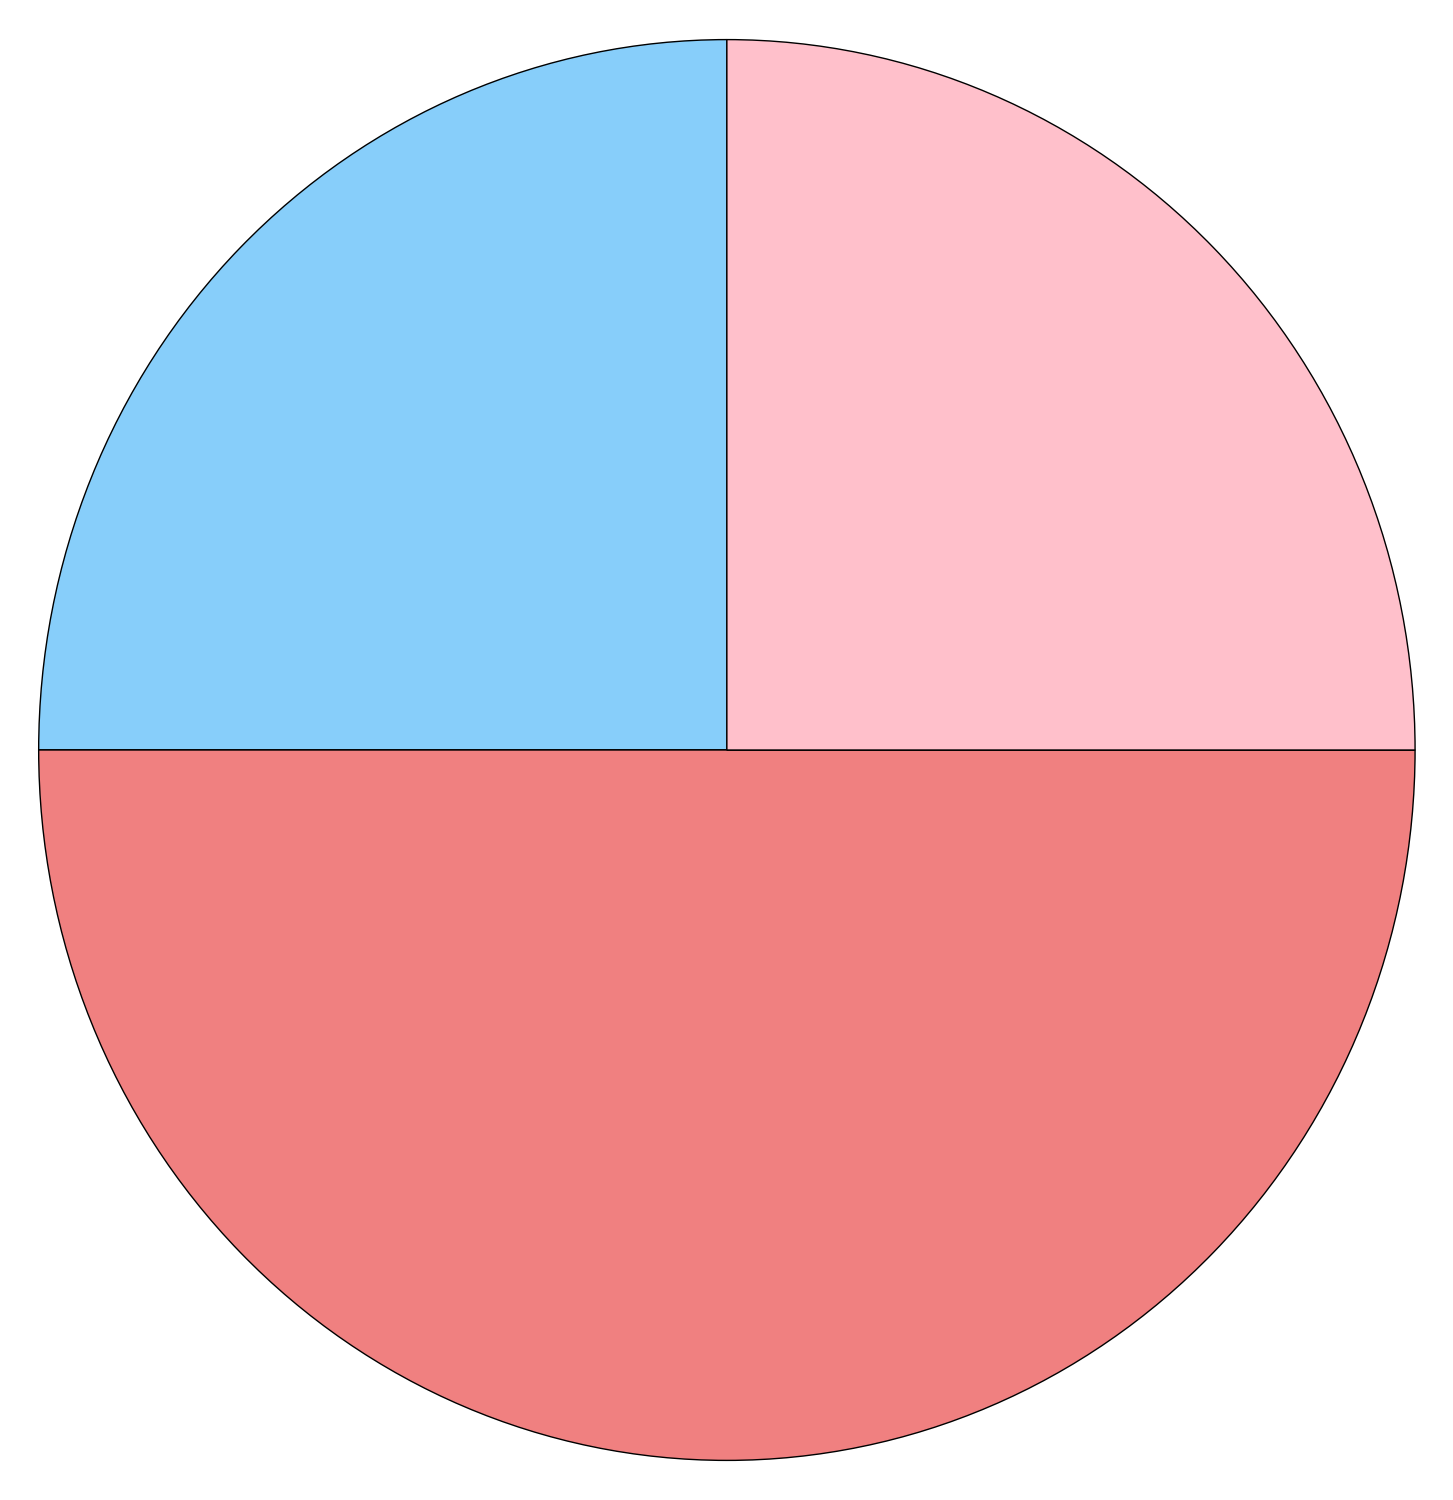
\includegraphics[width=\textwidth]{valencenon-EEGpearsonRgen}
    \caption{Pearson correlation}
  \end{subfigure}
  \hfill
  \begin{subfigure}[b]{0.3\textwidth}
    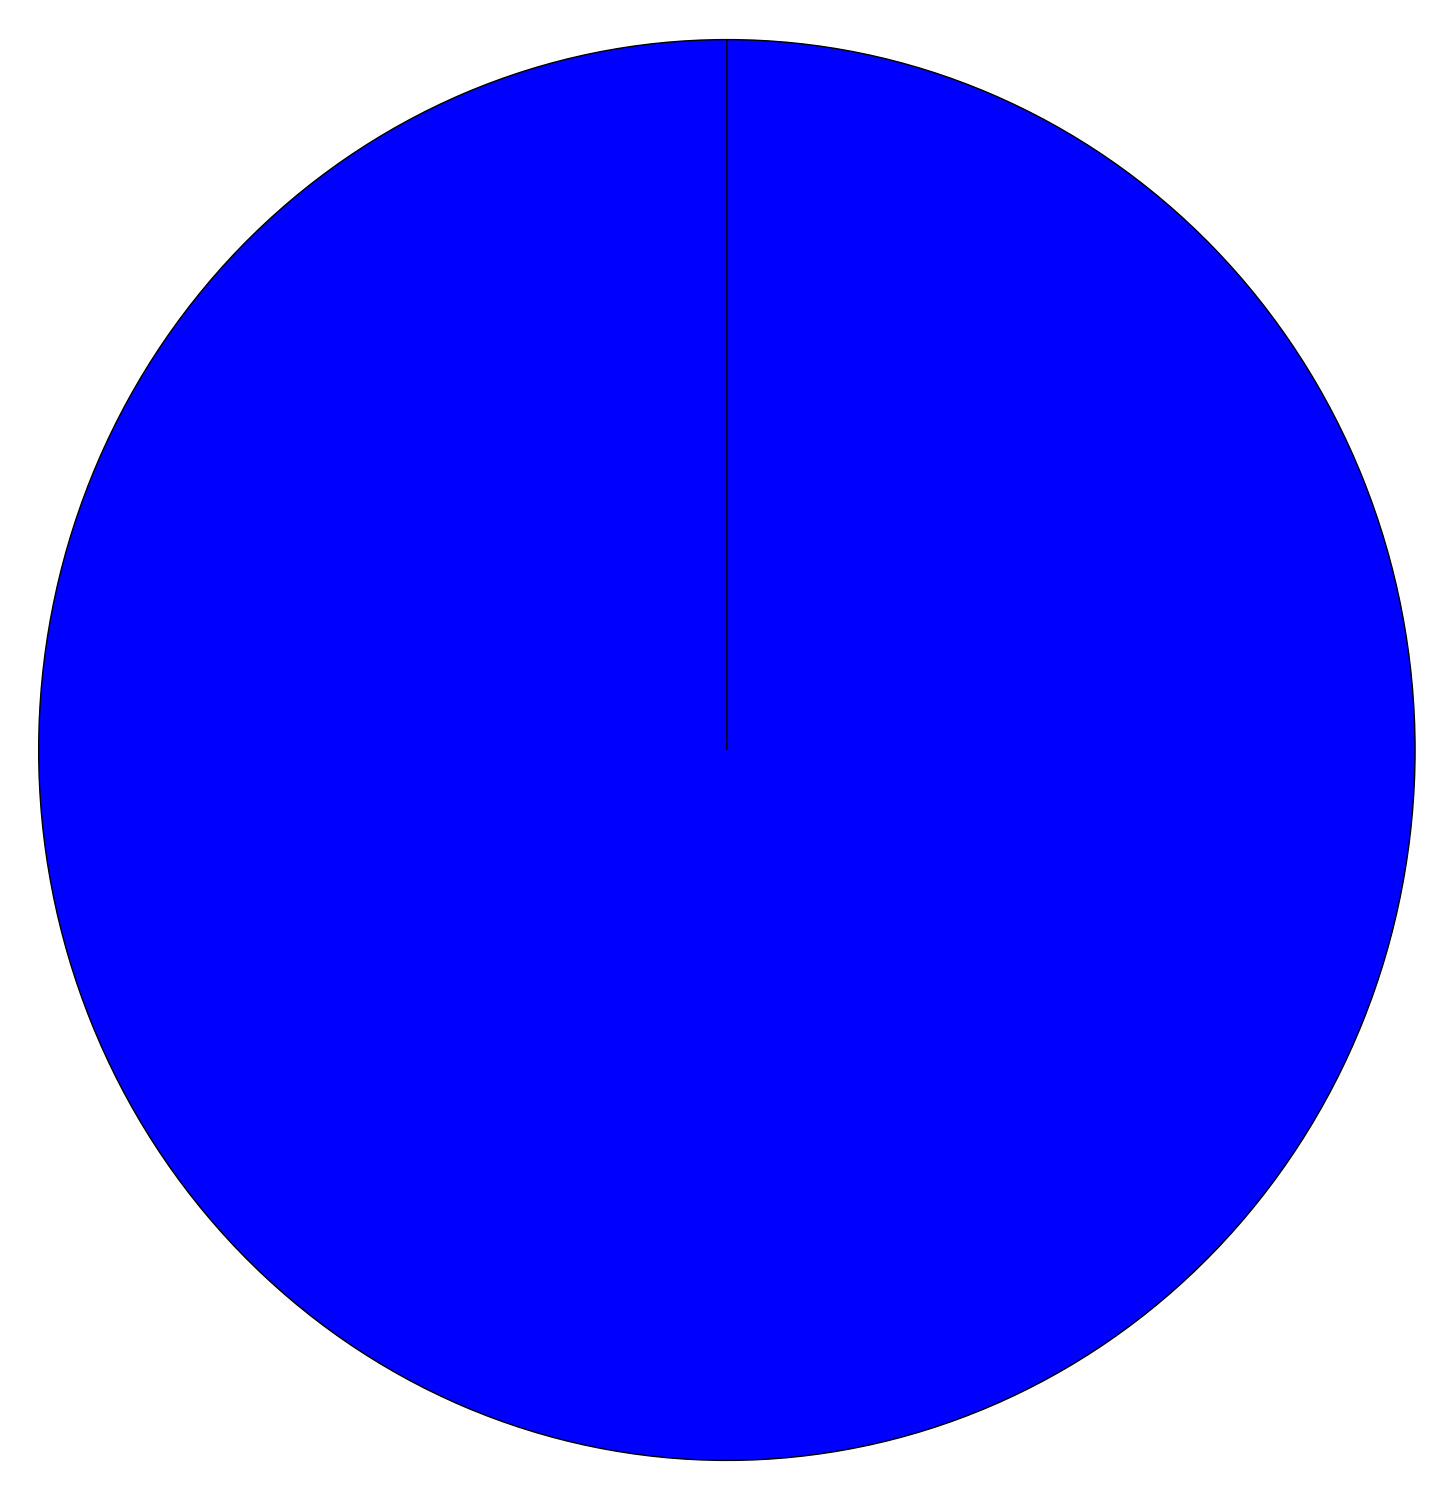
\includegraphics[width=\textwidth]{valencenon-EEGMutInfgen}
    \caption{Mutual information}
  \end{subfigure}
  \hfill
  \begin{subfigure}[b]{0.3\textwidth}
    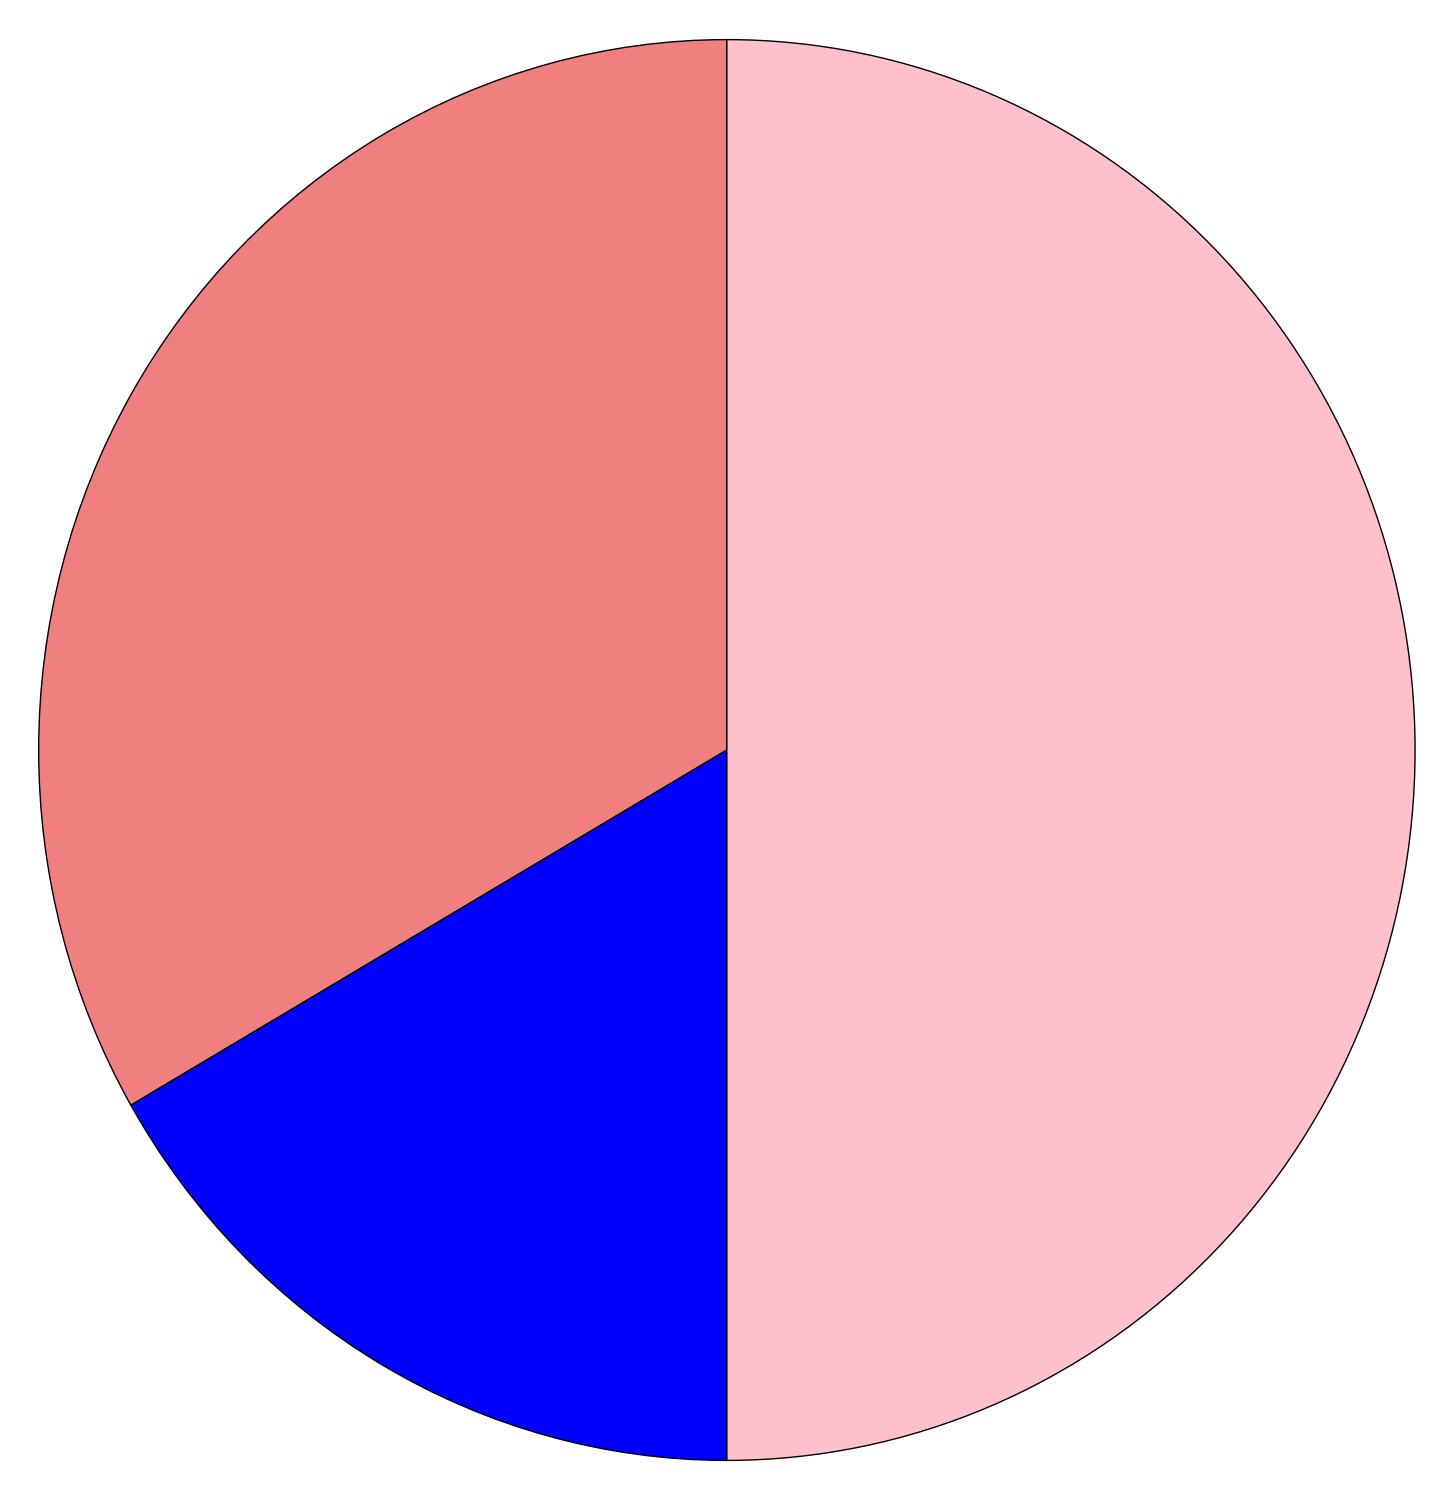
\includegraphics[width=\textwidth]{valencenon-EEGdCorrgen}
    \caption{Distance Correlation}
  \end{subfigure}
  
  \begin{subfigure}[b]{0.3\textwidth}
    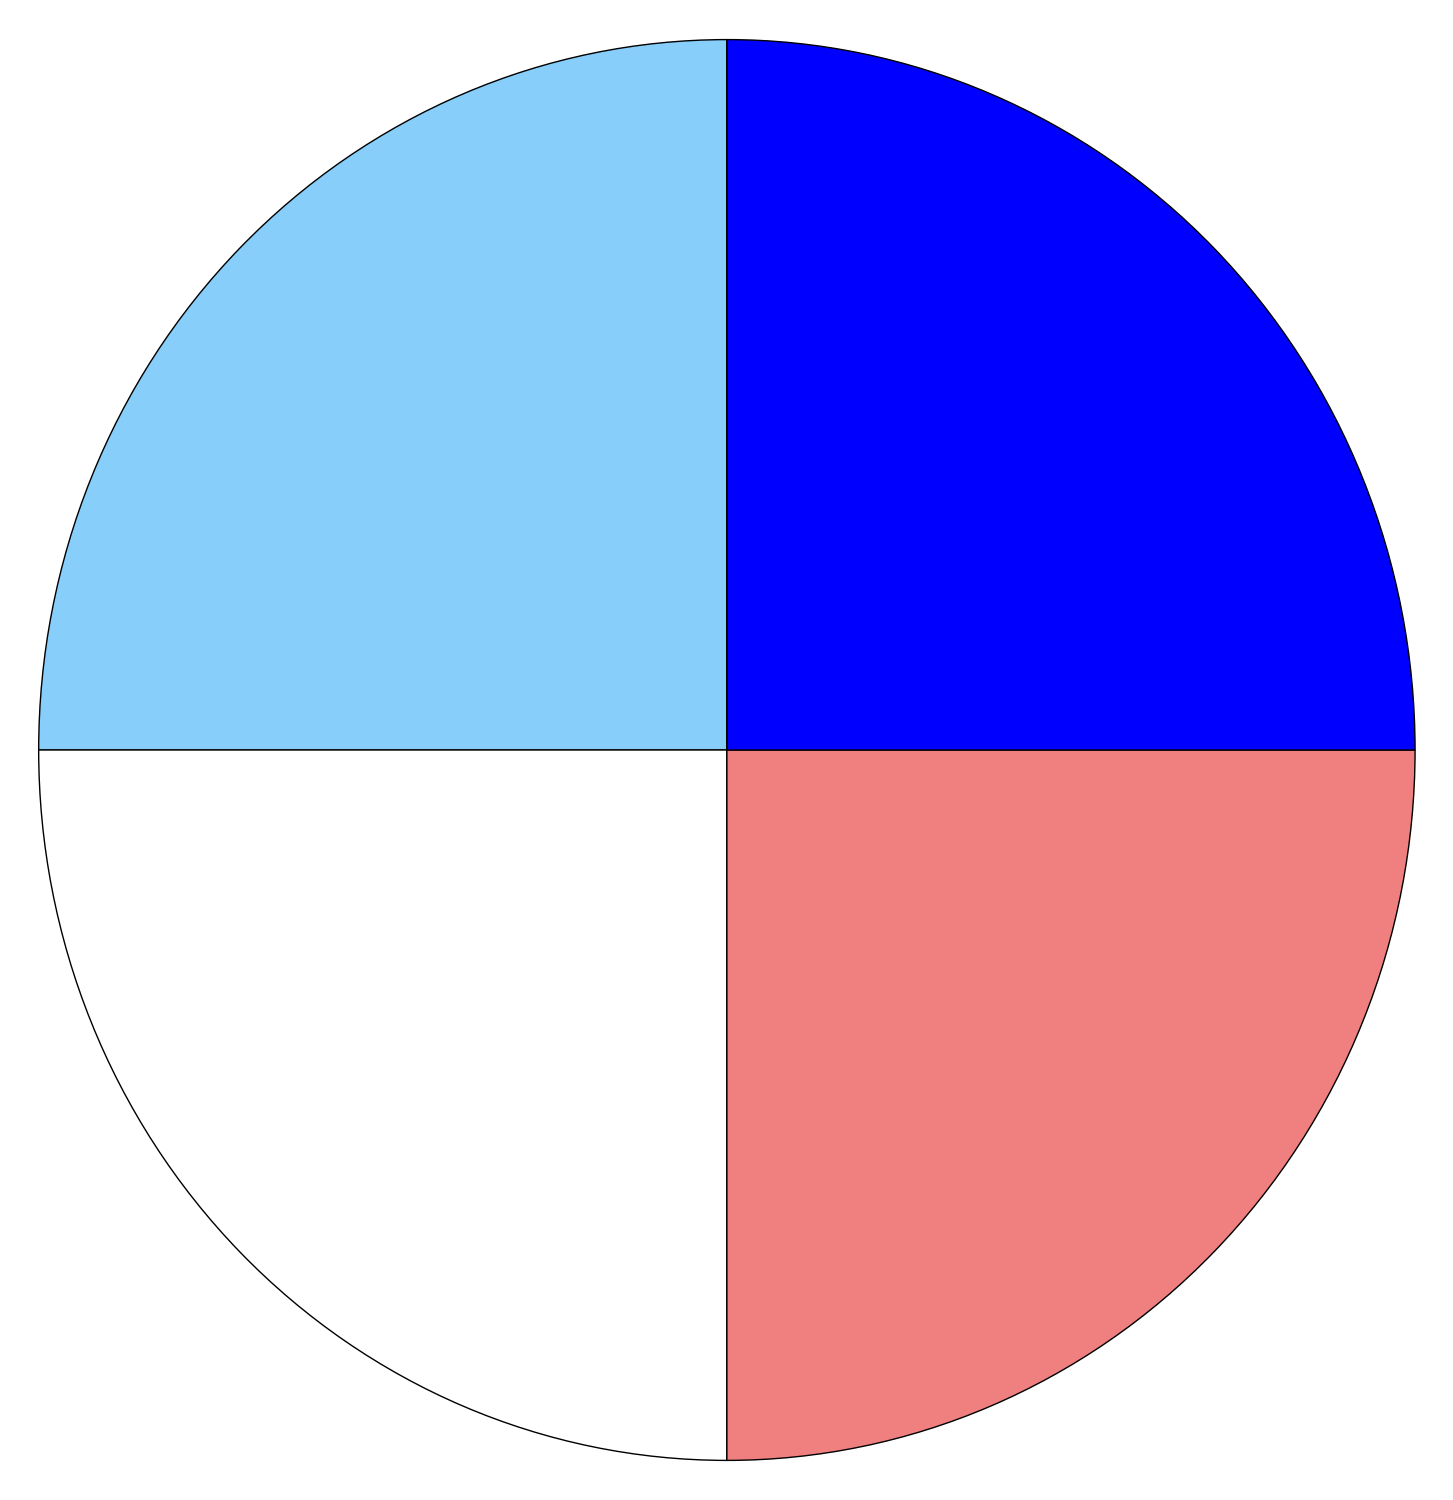
\includegraphics[width=\textwidth]{valencenon-EEGANOVAgen}
    \caption{ANOVA}
  \end{subfigure}
  \hfill
  \begin{subfigure}[b]{0.3\textwidth}
    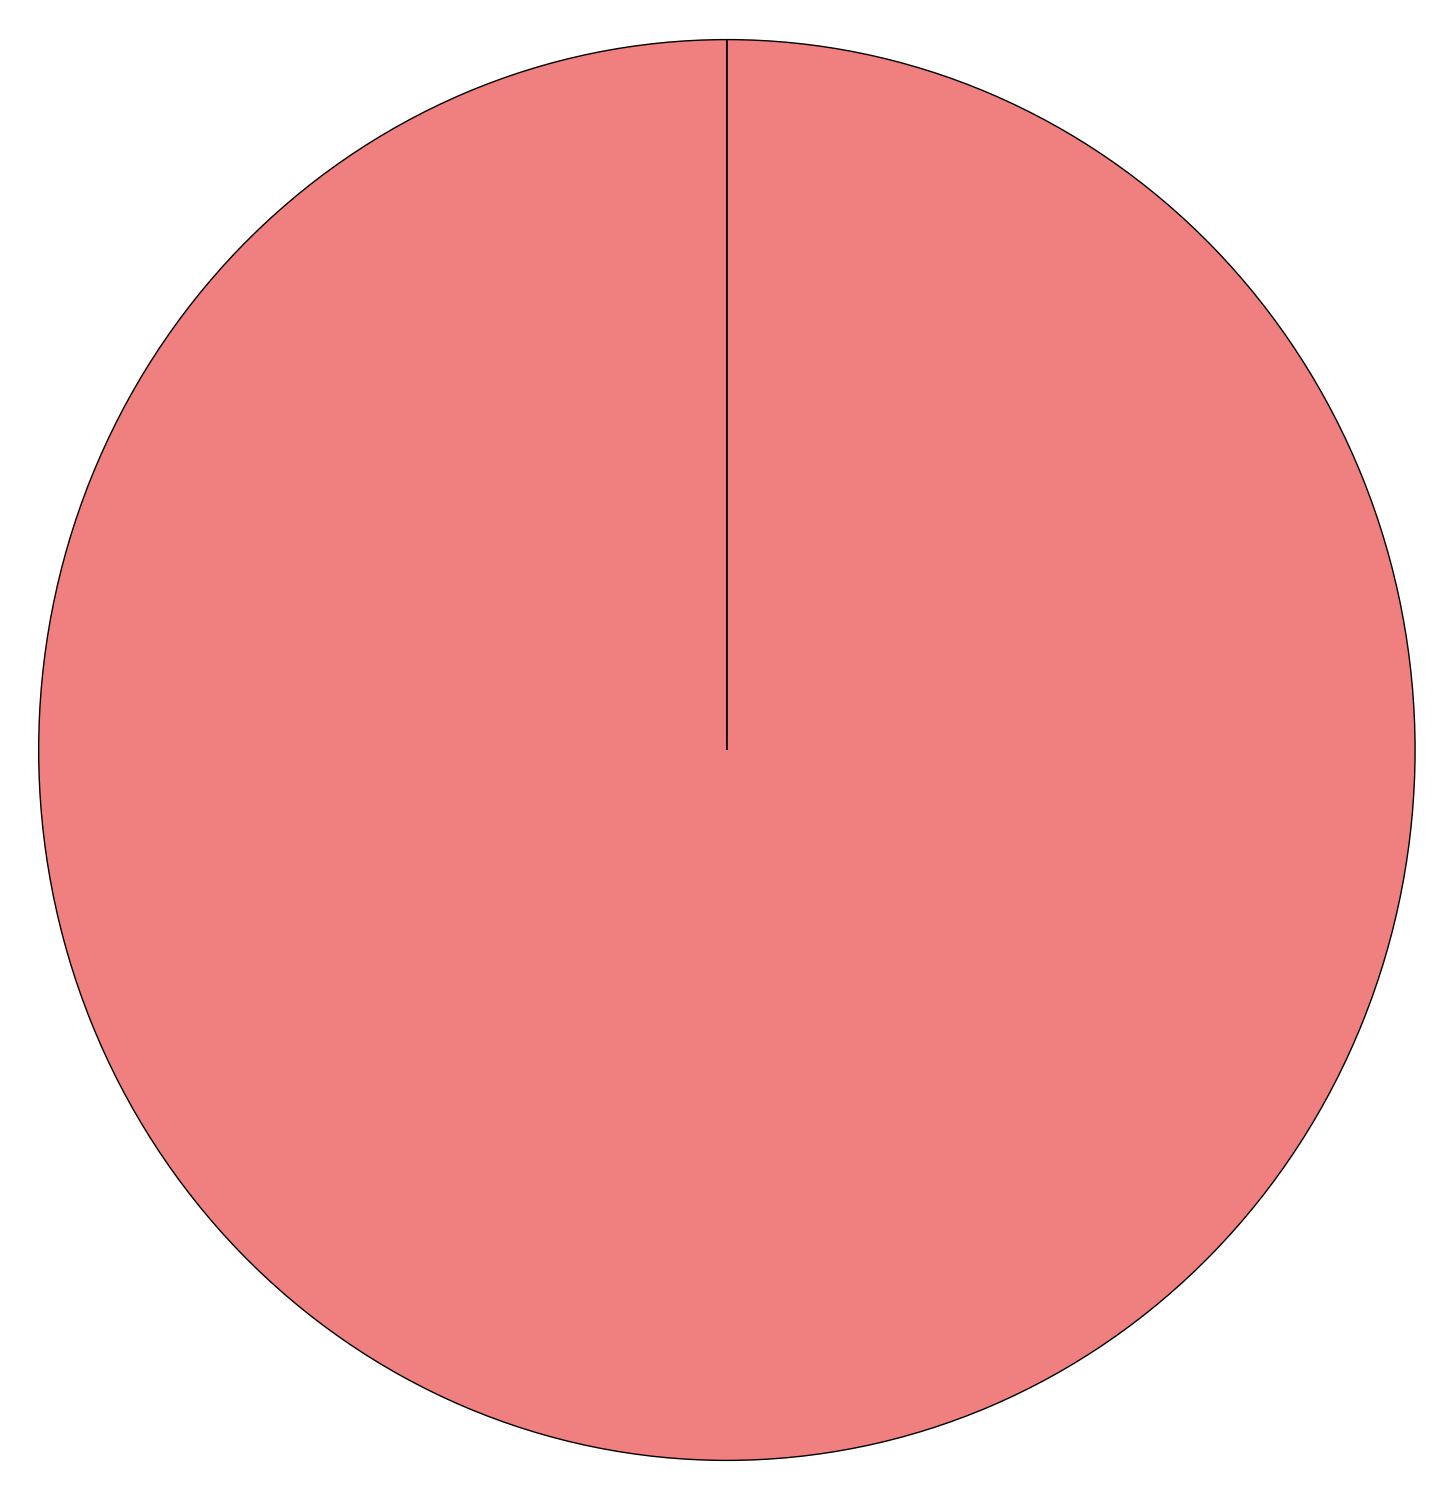
\includegraphics[width=\textwidth]{valencenon-EEGLRgen}
    \caption{Linear regression}
  \end{subfigure}
  \hfill
  \begin{subfigure}[b]{0.3\textwidth}
    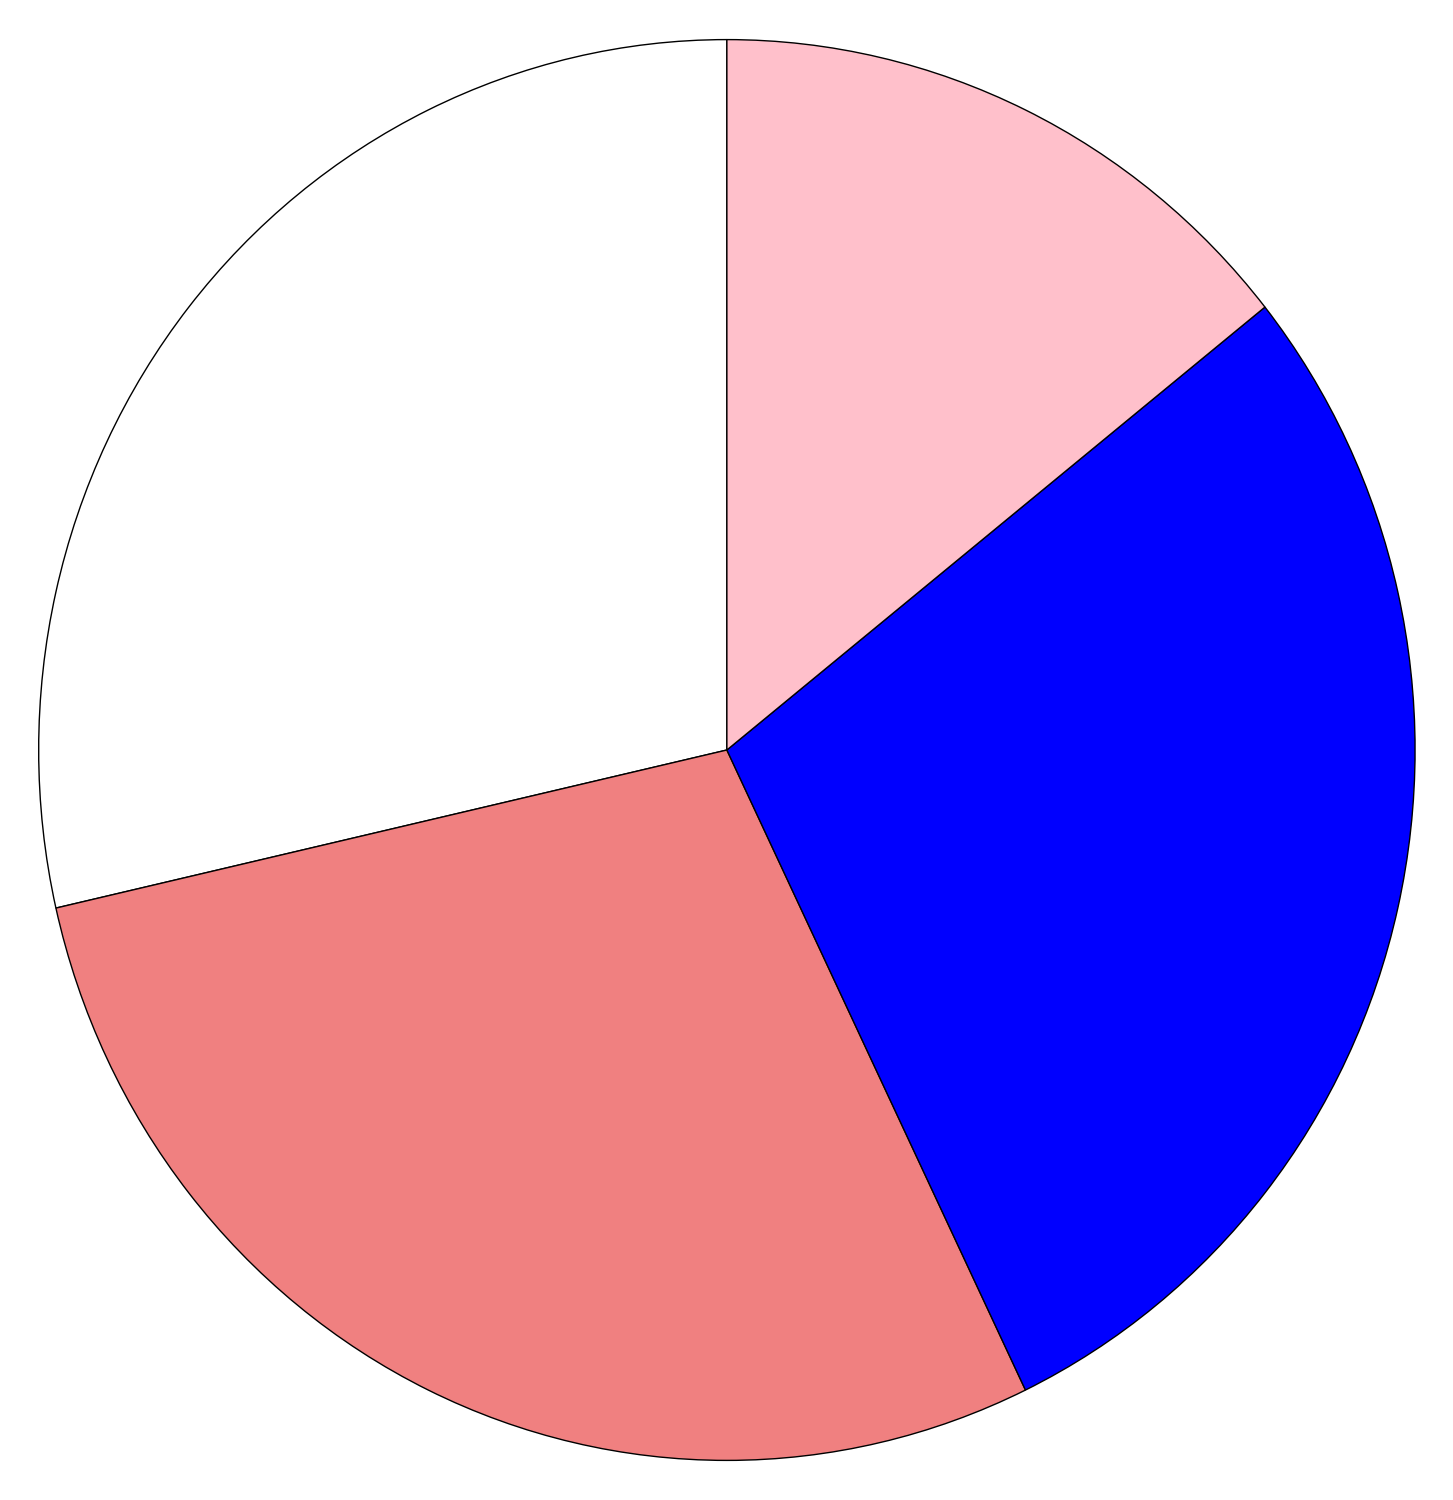
\includegraphics[width=\textwidth]{valencenon-EEGSVMgen}
    \caption{SVM}
  \end{subfigure}
  
  \begin{subfigure}[b]{0.3\textwidth}
    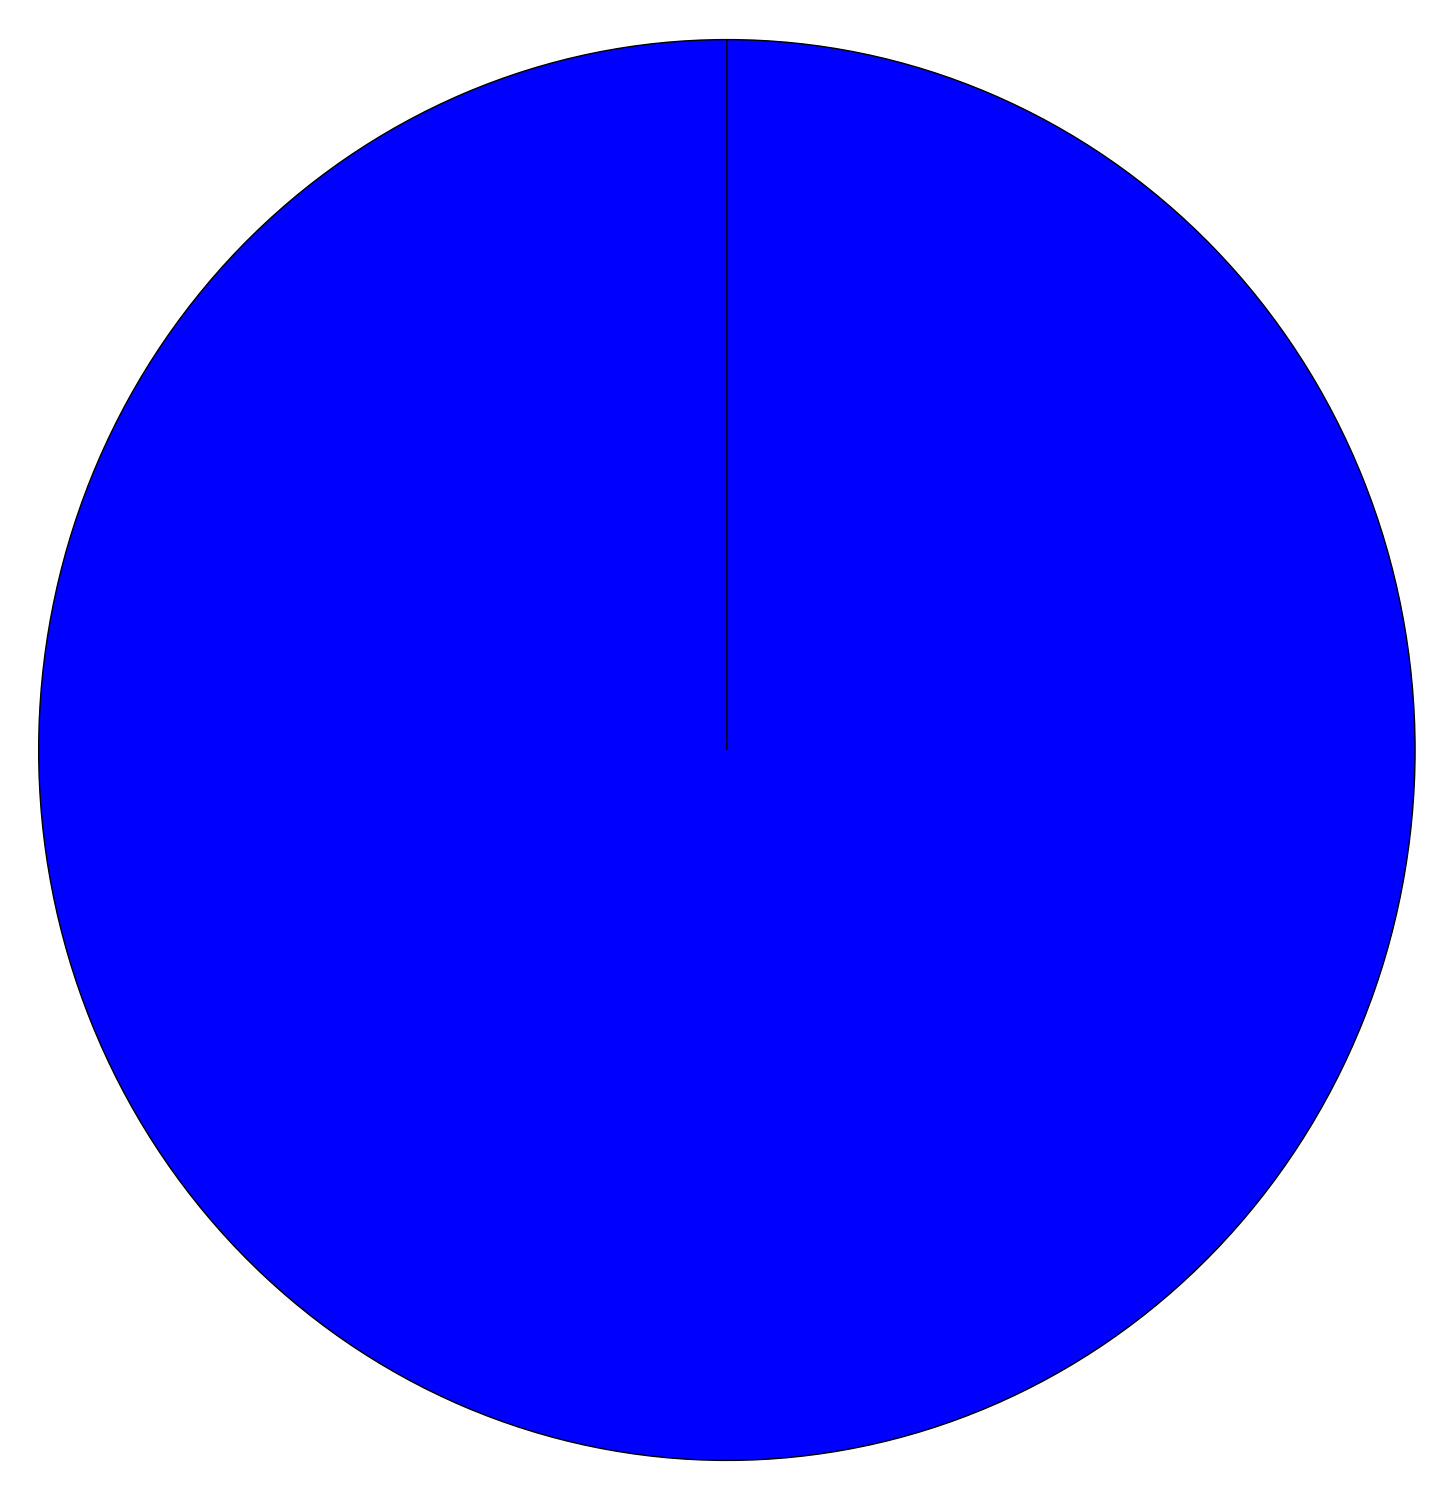
\includegraphics[width=\textwidth]{valencenon-EEGLDAgen}
    \caption{LDA}
  \end{subfigure}
  \hfill
  \begin{subfigure}[b]{0.3\textwidth}
    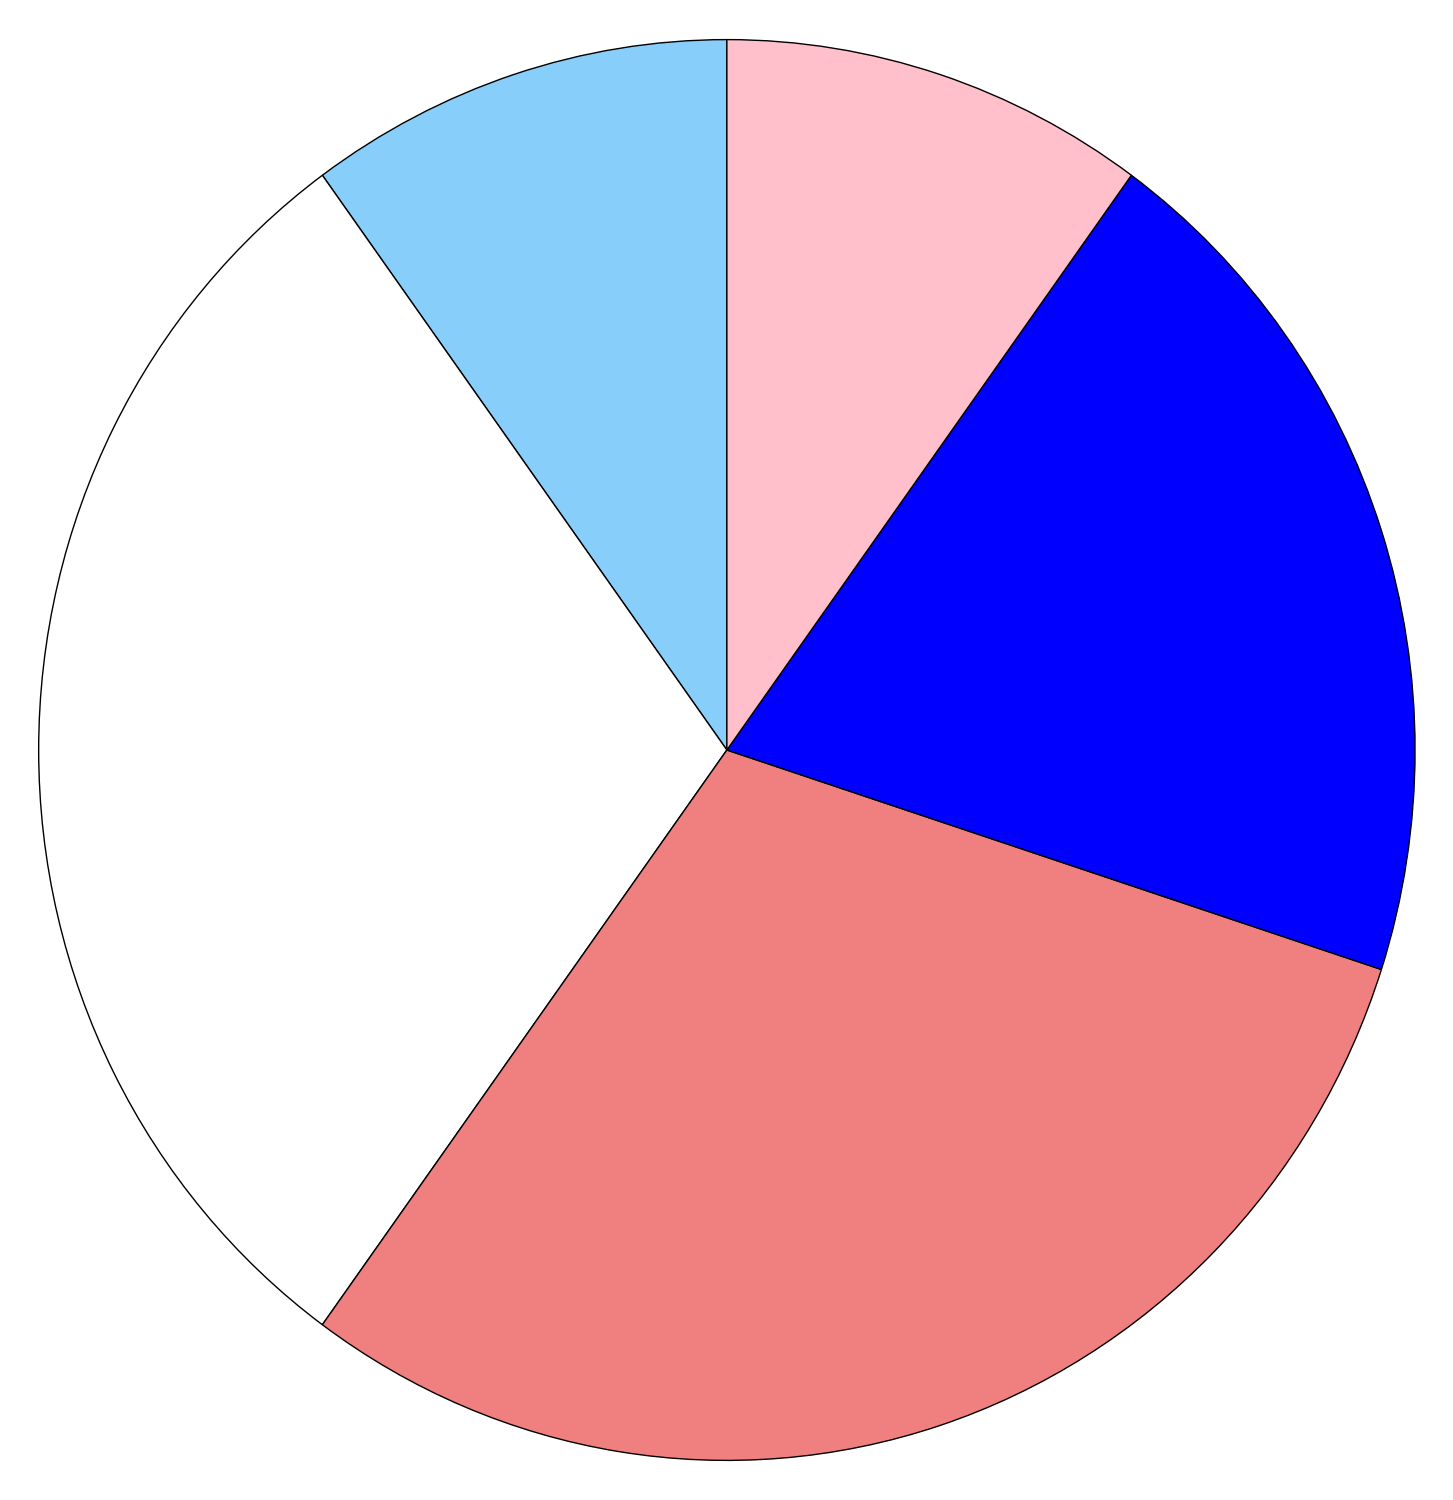
\includegraphics[width=\textwidth]{valencenon-EEGL1gen}
    \caption{Lasso regression}
  \end{subfigure}
  \hfill
  \begin{subfigure}[b]{0.3\textwidth}
    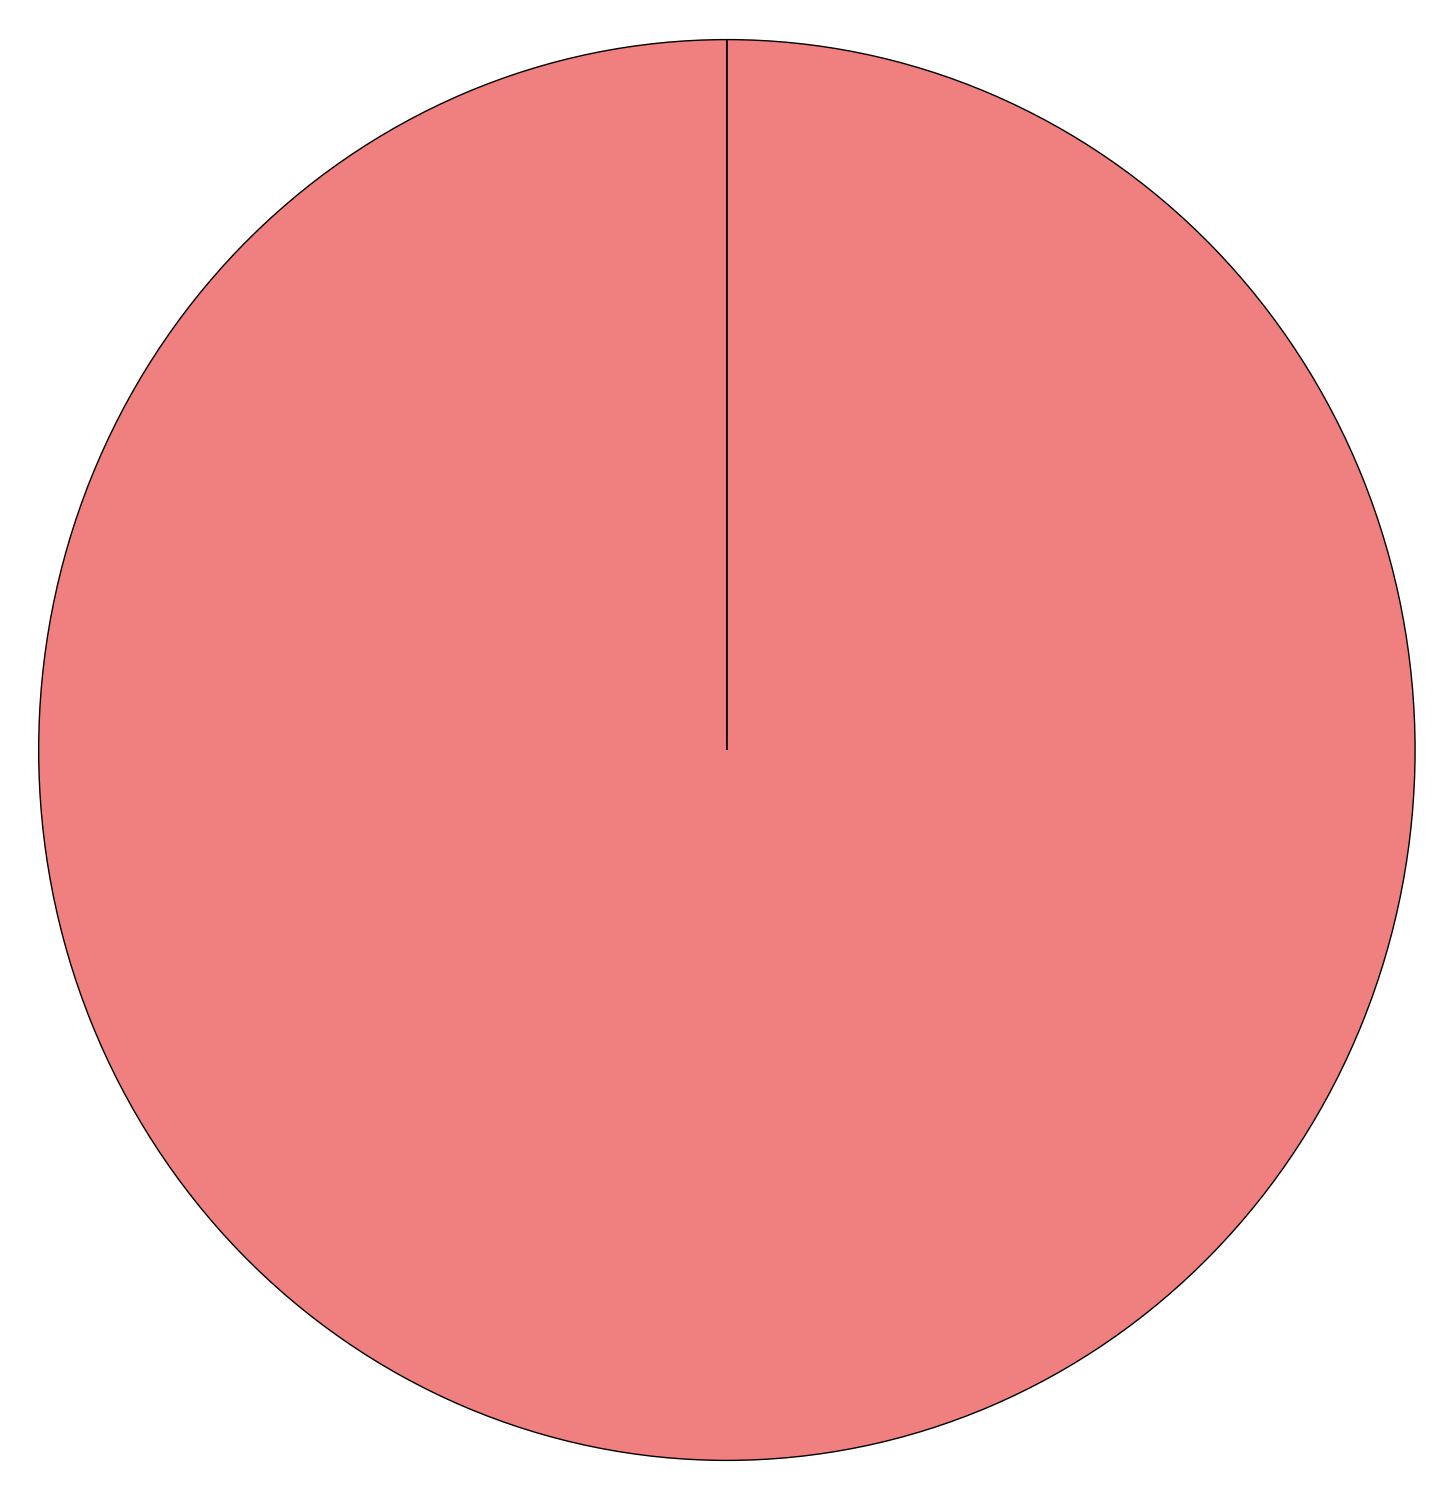
\includegraphics[width=\textwidth]{valencenon-EEGL2gen}
    \caption{Ridge regression}
  \end{subfigure}
  
  \begin{subfigure}[b]{0.3\textwidth}
    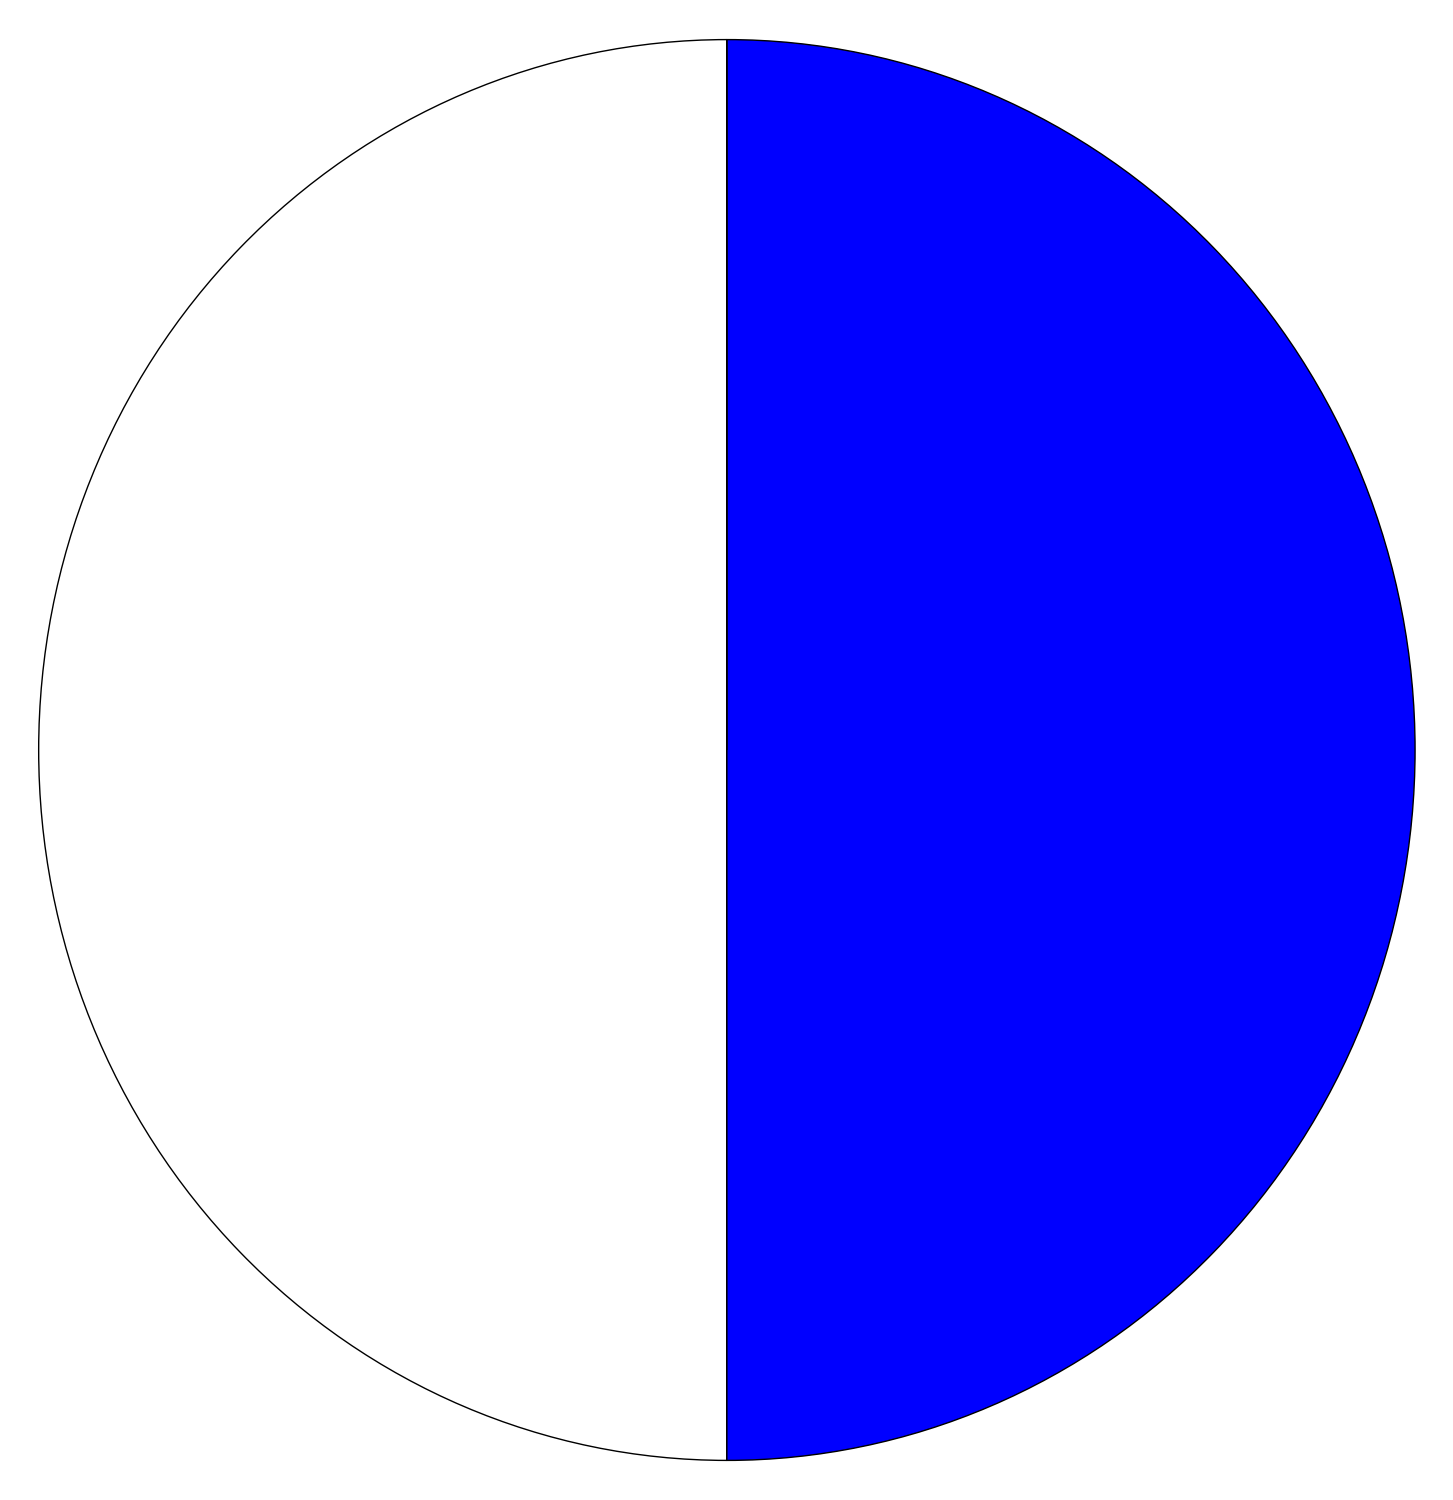
\includegraphics[width=\textwidth]{valencenon-EEGRFgen}
    \caption{Random forests}
  \end{subfigure}
  \hfill
  \begin{subfigure}[b]{0.3\textwidth}
    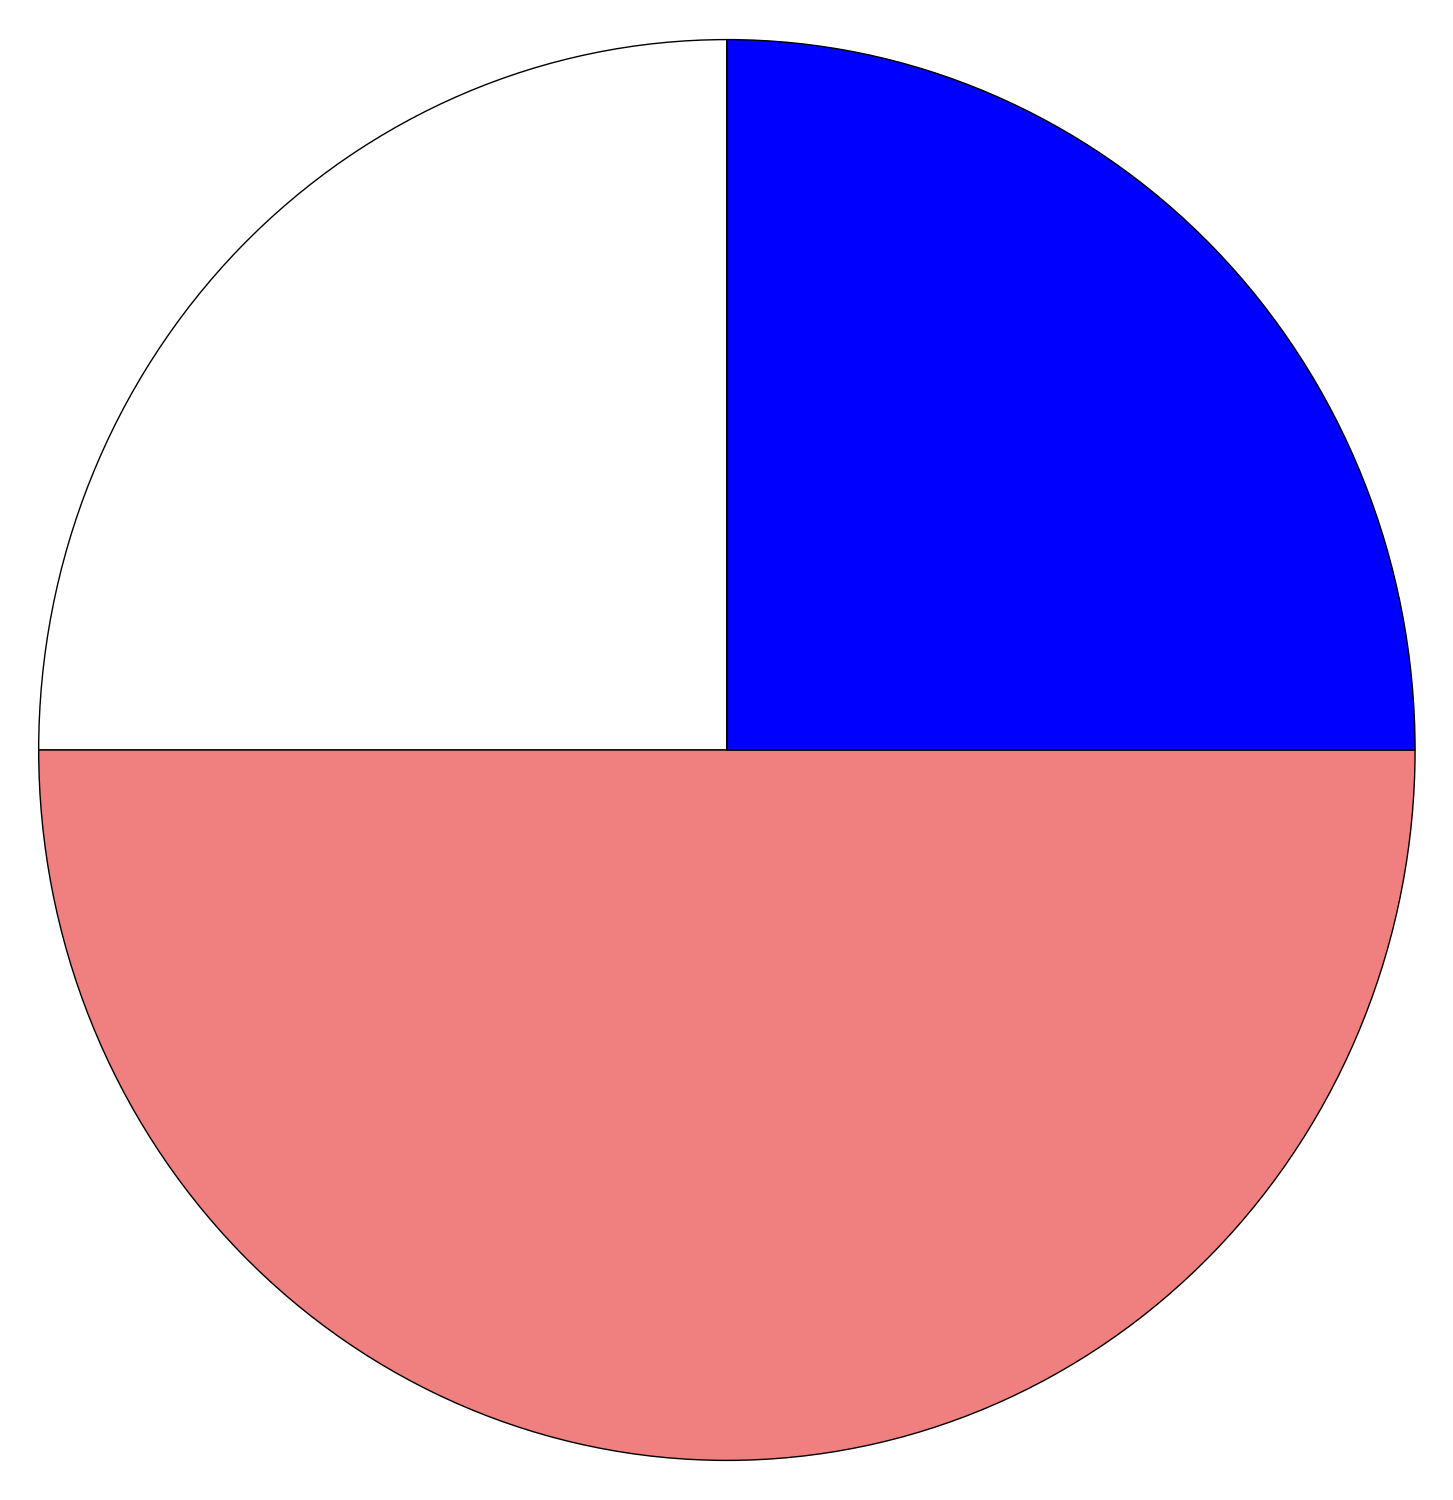
\includegraphics[width=\textwidth]{valencenon-EEGPCAgen}
    \caption{PCA}
  \end{subfigure}
  \hfill
  \begin{subfigure}[b]{0.3\textwidth}
    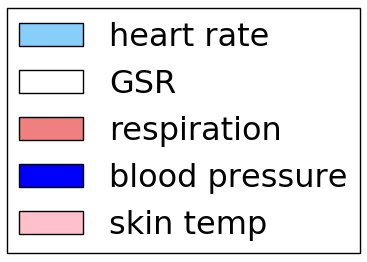
\includegraphics[width=\textwidth]{non-EEGlegend}
    \caption{Legend\label{valencepiesnon-EEGlegendgen}}
  \end{subfigure}
\end{figure}
\clearpage

\section{Important EEG channels}

The features used in the model build with the random forest feature selection for arousal are:
\begin{enumerate}
\item DE P4, gamma band
\item DE Cp1, gamma band
\item RCAU Fp2, O2, all bands
\item RCAU FC5, Cp5, all bands
\item DCAU Fz, Pz, all bands
\item fraction Cz, beta band
\item fraction P7, beta band
\end{enumerate}

For valence the features are:
\begin{enumerate}
\item DCAU Fz,Pz, beta band
\item DASM CP1,CP2, beta band
\item DE Pz, gamma band
\item DCAU Fz,Pz, gamma band
\item frac Fz, delta band
\item DE Fz, theta band
\item DCAU F4,P4, gamma band
\item frac P3, delta band
\end{enumerate}

In a cross-person setting, the DCAU features seem to perform well. These features are selected from front and posterior channels. However these results should be treated with caution, especially in case of valence, which only obtained a test accuracy of 55\%. If the classifier was not able to predict the emotional states well, one can doubt the selected features. 

\section{Stability}
TODO
%TODO